% !TEX root = ../Elements.tex
%%%%%%
% BOOK 8
%%%%%%
\pdfbookmark[0]{Book 8}{book8}
\pagestyle{empty}
\begin{center}
{\Huge ELEMENTS BOOK 8}\\
\spa\spa\spa
{\huge\it Continued Proportion\symbolfootnote[2]{The propositions contained in Books 7--9 are generally attributed to the
school of Pythagoras.}}
\end{center}
%\vspace{2cm}
%% Removed epsf size command
%\centerline{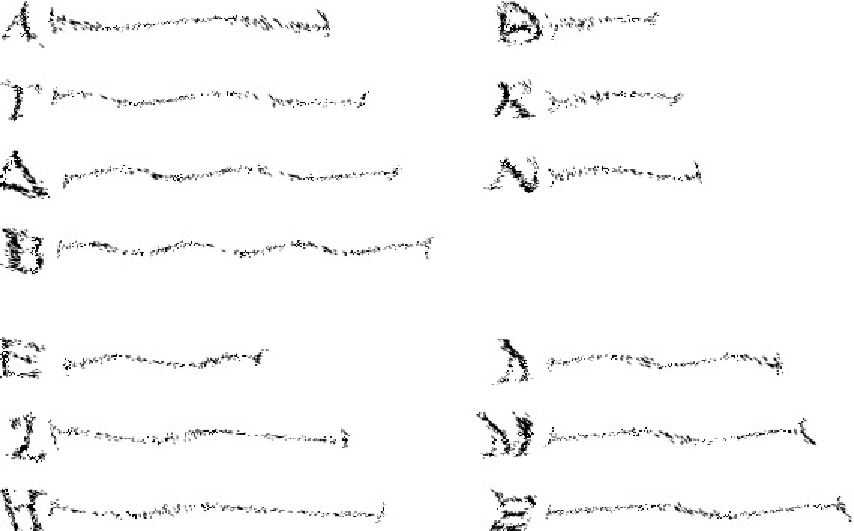
\includegraphics{Book08/front.pdf}}
\newpage

%%%%%%
% Prop 8.1
%%%%%%
\pdfbookmark[1]{Proposition 8.1}{pdf8.1}
\pagestyle{fancy}
\cfoot{\gr{\kern -.7pt }}
\lhead{\large\gr{ΣΤΟΙΘΕΙΩΝ \kern -.7pt {8}.}}
\rhead{\large ELEMENTS BOOK 8}
\begin{Parallel}{}{} 
\ParallelLText{
\begin{center}
{\large \ggn{1}.}
\end{center}\vspace*{-7pt}

\gr{Ἐὰν >ῶσιν ὁσοιδηποτοῦν ἀριθμοὶ ἑχῆξ ἀνάλογον, οἱ  δὲ >άκροι α\kern -.7pt  ὐτῶν πρῶτοι πρὸξ ἀλλήλουξ >ῶσιν, ἐλάθιστοί εἰσι τῶν τὸν
α\kern -.7pt  ὐτὸν λόγον ἐθόντων α\kern -.5pt  ὐτοῖξ.}\\

% Removed epsf size command
\centerline{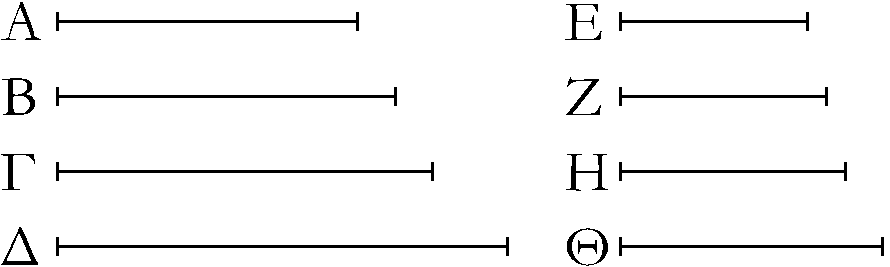
\includegraphics{Book08/fig01g.pdf}}

\gr{>'Εστωσαν ὁποσοιοῦν ἀριθμοὶ ἑχῆξ ἀνάλογον οἱ Α, Β, Γ,
Δ, οἱ δὲ >άκροι α\kern -.7pt  ὐτῶν οἱ Α, Δ, πρῶτοι πρὸξ ἀλλήλουξ
>έστωσαν; λέγω, <ότι οἱ Α, Β, Γ, Δ ἐλάθιστοί εἰσι
τῶν τὸν α\kern -.7pt  ὐτὸν λόγον ἐθόντων α\kern -.5pt  ὐτοῖξ.}

\gr{Εἰ γὰρ μ\kern -.7pt  ή, >έστωσαν ἐλάττονεξ τῶν Α, Β, Γ, Δ
οἱ Ε, Ζ, Η, Θ ἐν τῶ| α\kern -.7pt  ὐτῶ| λόγῳ >όντεξ α\kern -.5pt  ὐτοῖξ. καὶ
ἐπεὶ οἱ Α, Β, Γ, Δ ἐν τῶ| α\kern -.3pt  ὐτῶ| λόγῳ
εἰσὶ τοῖξ
Ε, Ζ, Η, Θ, καί ἐστιν >ίσον τὸ πλῆθοξ [τῶν Α, Β,
Γ, Δ] τῶ| πλήθει [τῶν Ε, Ζ, Η, Θ], δι> >ίσου >άρα
ἐστὶν ὡξ ὁ Α πρὸξ τὸν Δ, ὁ Ε πρὸξ τὸν Θ. οἱ δὲ Α, Δ
πρῶτοι, οἱ δὲ πρῶτοι καὶ ἐλάθιστοι, οἱ
δὲ ἐλάθιστοι ἀριθμοὶ μετροῦσι τοὺξ τὸν α\kern -.7pt  ὐτὸν λόγον
>έθονταξ ἰσάκιξ <ό τε μείζων τὸν μείζονα καὶ ὁ ἐλάσσων
τὸν ἐλάσσονα, τουτέστιν <ό τε ἡγούμενοξ τὸν ἡγούμενον
καὶ ὁ ἑπόμενοξ τὸν ἑπόμενον. μετρεῖ >άρα ὁ Α τὸν
Ε ὁ μείζων τὸν ἐλάσσονα; <όπερ ἐστὶν ἀδύνατον. οὐκ
>άρα  οἱ Ε, Ζ, Η, Θ ἐλάσσονεξ >όντεξ τῶν Α, Β,
Γ, Δ ἐν τῶ| α\kern -.7pt  ὐτῶ| λόγῳ εἰσὶν α\kern -.7pt  ὐτοῖξ. οἱ Α, Β, Γ,
Δ >άρα ἐλάθιστοί εἰσι τῶν τὸν α\kern -.7pt  ὐτὸν λόγον ἐθόντων α\kern -.7pt  ὐτοῖξ;
<όπερ >έδει δεῖχαι.}}

\ParallelRText{
\begin{center}
{\large Proposition 1}
\end{center}

If there are any multitude whatsoever of continuously proportional
numbers, and the outermost of them are prime to one another, then
the (numbers) are the least of those (numbers) having the same ratio as them.

% Removed epsf size command
\centerline{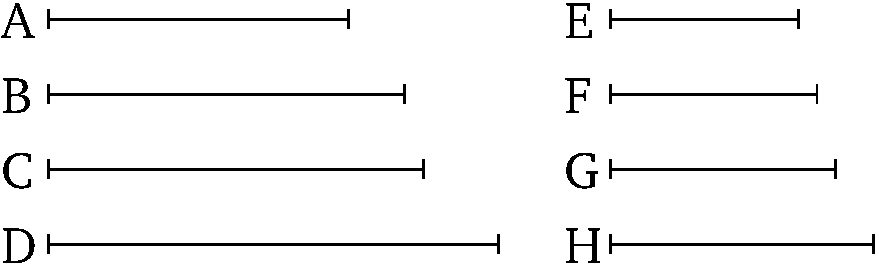
\includegraphics{Book08/fig01e.pdf}}

Let $A$, $B$, $C$,  $D$ be any multitude whatsoever of continuously proportional
numbers. And let the outermost of them, $A$ and $D$, be prime to
one another. I say that $A$, $B$, $C$, $D$ are the least of those
(numbers) having the same ratio as them.

For if not, let $E$, $F$, $G$, $H$ be less than $A$, $B$, $C$,  $D$ (respectively),
being in the same ratio as them. And since $A$, $B$, $C$, $D$ are
in the same ratio as $E$, $F$, $G$,  $H$, and
the multitude [of $A$, $B$, $C$, $D$] is equal to the
multitude [of $E$, $F$, $G$, $H$], thus, via equality, as
$A$ is to $D$, (so) $E$ (is) to $H$ [Prop.~7.14]. 
And $A$ and $D$ (are) prime (to one another). And prime (numbers are)
also the least of those (numbers having the same ratio as them) [Prop.~7.21]. And the least numbers measure those
(numbers) having the same ratio (as them) an equal number of times, the
greater (measuring) the greater, and the lesser the lesser---that is to say,
the leading (measuring) the leading, and the following the following [Prop.~7.20]. Thus, $A$ measures $E$, the
greater (measuring) the lesser. The very thing is impossible. Thus, $E$,
$F$, $G$,  $H$, being less than $A$, $B$, $C$, $D$, are not
in the same ratio as them. Thus, $A$, $B$, $C$,  $D$ are the least of those
(numbers) having the same ratio as them. (Which is) the very thing it was required to show.}
\end{Parallel}

%%%%%%
% Prop 8.2
%%%%%%
\pdfbookmark[1]{Proposition 8.2}{pdf8.2}
\begin{Parallel}{}{} 
\ParallelLText{
\begin{center}
{\large\ggn{2}.}
\end{center}\vspace*{-7pt}

\gr{Αριθμοὺξ εὑρεῖν ἑχῆξ ἀνάλογον ἐλαθίστουξ, <όσουξ >ὰν ἐπιτάχῃ
τιξ, ἐν τῶ| δοθέντι λόγῳ.}

\gr{>'Εστω ὁ δοθεὶξ λόγοξ ἐν ἐλάθίστοιξ ἀριθμοῖξ ὁ τοῦ Α πρὸξ
τὸν Β; δεῖ δὴ ἀριθμοὺξ εὑρεῖν ἑχῆξ ἀνάλογον ἐλαθίστουξ,
<όσουξ >άν τιξ ἐπιτάχῃ, ἐν τῶ| τοῦ Α πρὸξ τὸν Β
λόγῳ.}

\gr{Ἐπιτετάθθωσαν δὴ τέσσαρεξ, καὶ ὁ Α ἑαυτὸν πολλαπλασιάσαξ τὸν
Γ ποιείτω, τὸν δὲ Β πολλαπλασιάσαξ τὸν Δ ποιείτω, καὶ >έτι ὁ Β
 ἑαυτὸν πολλαπλασιάσαξ τὸν Ε ποιείτω,
καὶ >έτι ὁ Α τοὺξ Γ, Δ, Ε πολλαπλασιάσαξ τοὺξ Ζ, Η, Θ
ποιείτω, ὁ δὲ Β τὸν Ε πολλαπλασιάσαξ τὸν Κ ποιείτω.}

% Removed epsf size command
\centerline{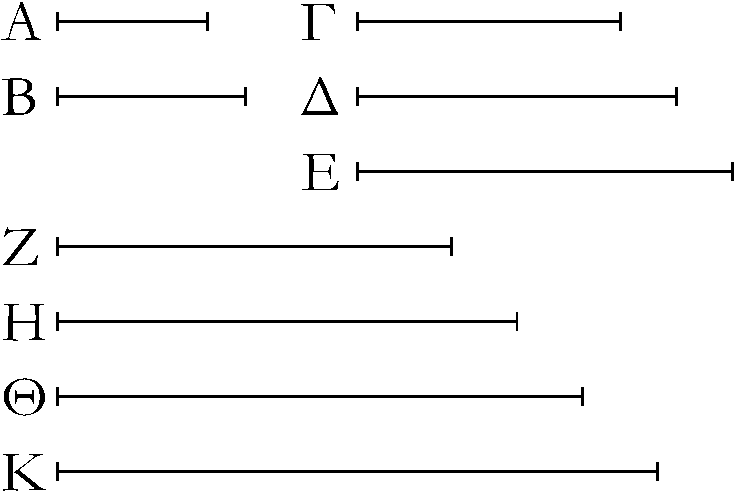
\includegraphics{Book08/fig02g.pdf}}

\gr{Καὶ ἐπεὶ ὁ Α ἑαυτὸν μὲν πολλαπλασιάσαξ τὸν Γ πεποίηκεν,
τὸν δὲ Β πολλαπλασιάσαξ τὸν Δ πεποίηκεν, >έστιν >άρα ὡξ ὁ
Α πρὸξ τὸν Β, [ο<ύτωξ] ὁ Γ πρὸξ τὸν Δ. πάλιν, ἐπεὶ ὁ μὲν
Α τὸν Β πολλαπλασιάσαξ τὸν Δ πεποίηκεν, ὁ δὲ Β ἑαυτὸν
πολλαπλασιάσαξ τὸν Ε πεποίηκεν, ἑκάτεροξ >άρα τῶν Α, Β τὸν Β
πολλαπλασιάσαξ ἑκάτερον τῶν Δ, Ε πεποίηκεν. >έστιν >άρα ὡξ ὁ Α
πρὸξ τὸν Β, ο<ύτωξ ὁ Δ πρὸξ τὸν Ε. ἀλλ> ὡξ ὁ Α πρὸξ τὸν Β,
ὁ Γ πρὸξ τὸν Δ; καὶ ὡξ >άρα ὁ Γ πρὸξ τὸν Δ, ὁ Δ πρὸξ τὸν
Ε. καὶ ἐπεὶ ὁ Α τοὺξ Γ, Δ πολλαπλασιάσαξ τοὺξ Ζ, Η πεποίηκεν, >έστιν >άρα
ὡξ ὁ Γ πρὸξ τὸν Δ, [ο<ύτωξ] ὁ Ζ πρὸξ τὸν Η. ὡξ δὲ ὁ Γ πρὸξ
τὸν Δ, ο<ύτωξ >ῆν ὁ Α πρὸξ τὸν Β; καὶ ὡξ >άρα ὁ Α πρὸξ τὸν
Β, ὁ Ζ πρὸξ τὸν Η. πάλιν, ἐπεὶ ὁ Α τοὺξ Δ, Ε πολλαπλασιάσαξ τοὺξ
Η, Θ πεποίηκεν, >έστιν >άρα ὡξ ὁ Δ πρὸξ τὸν Ε, ὁ Η πρὸξ τὸν Θ. ἀλλ>
ὡξ ὁ Δ πρὸξ τὸν Ε, ὁ Α πρὸξ τὸν Β. καὶ ὡξ >άρα ὁ Α πρὸξ τὸν Β,
ο<ύτωξ ὁ Η πρὸξ τὸν Θ. καὶ ἐπεὶ οἱ Α, Β τὸν Ε πολλαπλασιάσαντεξ
τοὺξ Θ, Κ πεποιήκασιν, >έστιν >άρα ὡξ ὁ Α πρὸξ τὸν Β, ο<ύτωξ ὁ Θ
πρὸξ τὸν Κ. ἀλλ> ὡξ ὁ Α πρὸξ τὸν Β, ο<ύτωξ <ό τε Ζ πρὸξ τὸν Η
καὶ ὁ Η πρὸξ τὸν Θ. καὶ ὡξ >άρα ὁ Ζ πρὸξ τὸν Η, ο<ύτωξ <ό
τε Η πρὸξ τὸν Θ καὶ ὁ Θ πρὸξ τὸν Κ; οἱ Γ, Δ, Ε >άρα καὶ οἱ Ζ, Η,
Θ, Κ ἀνάλογόν εἰσιν ἐν τῶ| τοῦ Α πρὸξ τὸν Β λόγῳ. λέγω δή,
<ότι καὶ ἐλάθιστοι. ἐπεὶ γὰρ οἱ Α, Β ἐλάθιστοί εἰσι τῶν τὸν α\kern -.7pt  ὐτὸν
λόγον ἐθόντων α\kern -.7pt  ὐτοῖξ, οἱ δὲ ἐλάθιστοι τῶν τὸν α\kern -.5pt  ὐτὸν λόγον
ἐθόντων πρῶτοι πρὸξ ἀλλήλουξ εἰσίν, οἱ Α, Β >άρα πρῶτοι πρὸξ
ἀλλήλουξ εἰσίν. καὶ ἑκάτεροξ μὲν τῶν Α, Β ἑαυτὸν πολλαπλασιάσαξ
ἑκάτερον τῶν Γ, Ε πεποίηκεν, ἑκάτερον δὲ τῶν Γ, Ε πολλαπλασιάσαξ
ἑκάτερον τῶν Ζ, Κ πεποίηκεν; οἱ Γ, Ε >άρα καὶ οἱ Ζ, Κ πρῶτοι
πρὸξ ἀλλήλουξ εἰσίν. ἒαν δὲ >ῶσιν ὁποσοιοῦν ἀριθμοὶ
ἑχῆξ ἀνάλογον, οἱ δὲ >άκροι α\kern -.3pt  ὐτῶν πρῶτοι πρὸξ ἀλλήλουξ
>ῶσιν, ἐλάθιστοί εἰσι τῶν τὸν α\kern -.7pt  ὐτὸν λόγον ἐθόντων α\kern -.7pt  ὐτοῖξ.
οἱ Γ, Δ, Ε >άρα καὶ οἱ Ζ, Η, Θ, Κ ἐλάθιστοί εἰσι τῶν τὸν α\kern -.7pt  ὐτὸν
λόγον ἐθόντων τοῖξ Α, Β; <όπερ >έδει δεῖχαι.}\\

\begin{center}
{\large \gr{Πόρισμα}.}
\end{center}\vspace*{-7pt}

\gr{Ἐκ δὴ τούτου φανερόν, <ότι ἒαν τρεῖξ ἀριθμοὶ ἑχῆξ ἀνάλογον
ἐλάθιστοι >ῶσι τῶν τὸν α\kern -.7pt  ὐτὸν λόγον ἐθόντων α\kern -.7pt  ὐτοῖξ, οἱ
>άκρον α\kern -.5pt  ὐτῶν τετράγωνοί εἰσιν, ἒαν δὲ τέσσαρεξ, κύβοι.
}}

\ParallelRText{
\begin{center}
{\large Proposition 2}
\end{center}

To find the least numbers, as many as may be prescribed,  (which are) continuously proportional
in a given ratio.

Let the given ratio, (expressed) in the least numbers, be that of $A$ to $B$.
So it is required to find the least numbers, as many as may be prescribed, 
(which are) in the ratio of $A$ to $B$. 

Let four (numbers) be prescribed. And let $A$ make $C$ (by) multiplying itself, and let it make $D$ (by) multiplying $B$.
And, further, let $B$ make $E$ (by) multiplying itself. And, further, 
let $A$ make $F$, $G$,  $H$ (by) multiplying $C$, $D$,  $E$. And let $B$ make $K$ (by) multiplying $E$.

% Removed epsf size command
\centerline{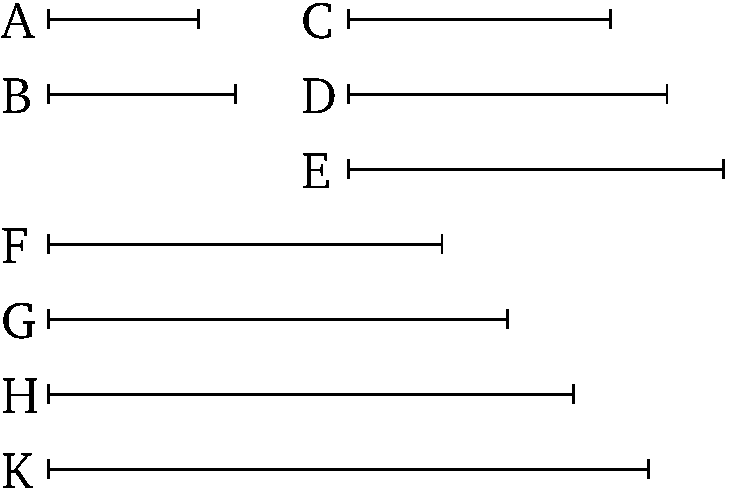
\includegraphics{Book08/fig02e.pdf}}

And since $A$ has made $C$ (by) multiplying itself, and has made $D$ (by)
multiplying $B$, thus as $A$ is to $B$, [so] $C$ (is) to $D$ [Prop.~7.17]. Again, since $A$ has made $D$
(by) multiplying $B$, and $B$ has made $E$ (by) multiplying itself,
 $A$, $B$ have thus made  $D$, $E$, respectively, (by)
multiplying $B$.  Thus, as $A$ is to $B$, so $D$ (is) to $E$ [Prop.~7.18]. But, as $A$ (is) to $B$, (so)
$C$ (is) to $D$. And thus as $C$ (is) to $D$, (so) $D$ (is) to $E$.
And since $A$ has made $F$, $G$ (by) multiplying $C$, $D$, thus as $C$ is to $D$, [so] $F$ (is) to $G$ [Prop.~7.17]. And as $C$ (is) to $D$, so
$A$ was to $B$. And thus as $A$ (is) to $B$, (so) $F$ (is) to $G$. Again,
since $A$ has made $G$, $H$ (by) multiplying $D$, $E$, thus as $D$ is to $E$, (so) $G$ (is) to $H$ [Prop.~7.17]. But, as $D$ (is) to $E$, (so) $A$ (is)
to $B$.  And thus as $A$ (is) to $B$, so $G$ (is) to $H$. And since
$A$, $B$ have made $H$, $K$ (by) multiplying
$E$, thus as $A$ is to $B$, so $H$ (is) to $K$. But, as $A$ (is) to $B$, so
$F$ (is) to $G$, and $G$ to $H$.  And thus as $F$ (is) to $G$, so $G$ (is)
to $H$, and $H$ to $K$. Thus, $C$, $D$, $E$ and $F$, $G$, $H$, $K$
are (both continuously) proportional in the ratio of $A$ to $B$. So I
say that (they are) also the least (sets of numbers continuously proportional in that
ratio). For since $A$ and $B$ are the least of those (numbers) having the
same ratio as them, and the least of those (numbers) having the same
ratio are prime to one another [Prop.~7.22],
$A$ and $B$ are thus prime to one another. And  $A$, $B$
have  made  $C$, $E$, respectively, (by) multiplying themselves, and have made $F$, $K$ by multiplying $C$, $E$, respectively. Thus,
$C$, $E$ and $F$, $K$ are prime to one another [Prop.~7.27]. And if there are any multitude whatsoever of continuously  proportional numbers, and the outermost
of them are prime to one another,  then the (numbers)  are the least of those
(numbers) having the same ratio as them [Prop.~8.1].
Thus, $C$, $D$, $E$ and $F$, $G$, $H$, $K$ are the least of those
(continuously proportional sets of numbers) having the same ratio as $A$ and $B$. (Which is) the very thing it was required to show.\\~\\

\begin{center}
{\large Corollary}
\end{center}\vspace*{-7pt}

So  it is clear, from this,  that if three continuously proportional numbers are the
least of those (numbers) having the same ratio as them then the outermost
of them are square, and, if four (numbers), cube.}
\end{Parallel}

%%%%%%
% Prop 8.3
%%%%%%
\pdfbookmark[1]{Proposition 8.3}{pdf8.3}
\begin{Parallel}{}{} 
\ParallelLText{
\begin{center}
{\large \ggn{3}.}
\end{center}\vspace*{-7pt}

\gr{Ἐὰν >ῶσιν ὁποσοιοῦν ἀριθμοὶ ἑχῆξ ἀνάλογον ἐλάθιστ\-οι
τῶν τὸν α\kern -.7pt  ὐτὸν λόγον ἐθόντων α\kern -.7pt  ὐτοῖξ, οἱ >άκροι
α\kern -.5pt  ὐτῶν πρῶτοι πρὸξ ἀλλήλουξ εἰσίν.}\\

% Removed epsf size command
\centerline{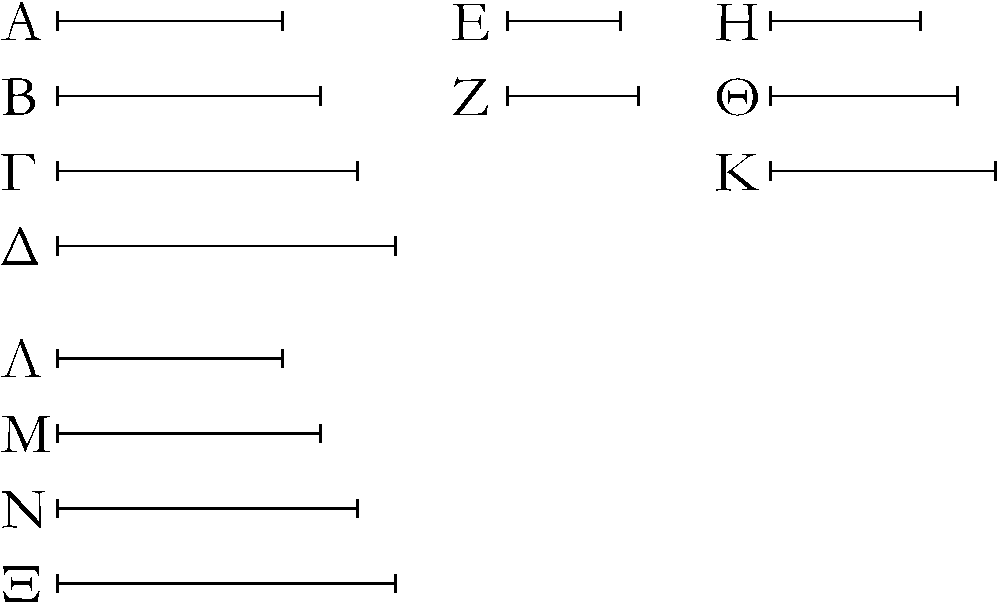
\includegraphics{Book08/fig03g.pdf}}

\gr{>'Εστωσαν ὁποσοιοῦν ἀριθμοὶ ἑχῆξ ἀνάλογον ἐλάθιστοι
τῶν τὸν α\kern -.7pt  ὐτὸν λόγον ἐθόντων α\kern -.7pt  ὐτοῖξ οἱ Α, Β, Γ, Δ;
λέγω, <ότι οἱ >άκροι α\kern -.5pt  ὐτῶν οἱ Α, Δ πρῶτοι πρὸξ ἀλλήλουξ
εἰσίν.}

\gr{Εἰλήφθωσαν γὰρ δύο μὲν ἀριθμοὶ ἐλάθιστοι ἐν τῶ| τῶν Α, Β, Γ,
Δ λόγῳ οἱ Ε, Ζ, τρεῖξ δὲ οἱ Η, Θ, Κ, καὶ ἑχῆξ ἑνὶ
πλείουξ, <έωξ τὸ λαμβανόμενον πλῆθοξ >ίσον γένηται τῶ| πλήθει
τῶν Α, Β, Γ, Δ. εἰλήφθωσαν καὶ >έστωσαν οἱ Λ, Μ, Ν, Χ.}

\gr{Καὶ ἐπεὶ οἱ Ε, Ζ ἐλάθιστοί εἰσι  τῶν τὸν α\kern -.7pt  ὐτὸν λόγον ἐθόντων
α\kern -.7pt  ὐτοῖξ, πρῶτοι πρὸξ ἀλλήλουξ εἰσίν. καὶ ἐπεὶ ἑκάτεροξ τῶν
Ε, Ζ ἑαυτὸν μὲν πολλαπλασιάσαξ ἑκάτερον τῶν Η, Κ πεποίηκεν,
ἑκάτερον δὲ τῶν Η, Κ πολλαπλασιάσαξ ἑκάτερον τῶν Λ, Χ
πεποίηκεν, καὶ οἱ Η, Κ >άρα καὶ οἱ Λ, Χ πρῶτοι πρὸξ
ἀλλήλουξ εἰσίν. καὶ ἐπεὶ οἱ Α, Β, Γ, Δ ἐλάθιστοί
εἰσι τῶν τὸν α\kern -.5pt  ὐτὸν λόγον ἐθόντων α\kern -.3pt  ὐτοῖξ, εἰσὶ
δὲ καὶ οἱ Λ, Μ, Ν, Χ ἐλάθιστοι ἐν τῶ| α\kern -.7pt  ὐτῶ| λόγῳ >όντεξ
τοῖξ Α, Β, Γ, Δ, καί ἐστιν >ίσον τὸ πλῆθοξ τῶν Α, Β, Γ, Δ τῶ|
πλήθει τῶν Λ, Μ, Ν, Χ, <έκαστοξ >άρα τῶν Α, Β, Γ, Δ ἑκάστῳ τῶν
Λ, Μ, Ν, Χ
 >ίσοξ ἐστίν; >ίσοξ >άρα ἐστὶν ὁ μὲν
Α τῶ| Λ, ὁ δὲ Δ τῶ| Χ. καί εἰσιν οἱ Λ, Χ πρῶτοι πρὸξ ἀλλήλουξ.
καὶ οἱ Α, Δ >άρα πρῶτοι πρὸξ ἀλλήλουξ εἰσίν; <όπερ
>έδει δεῖχαι.}}

\ParallelRText{
\begin{center}
{\large Proposition 3}
\end{center}

If there are any multitude whatsoever of continuously proportional
numbers (which are)  the least of those (numbers) having the same ratio as them then the outermost of them are prime to one another.

% Removed epsf size command
\centerline{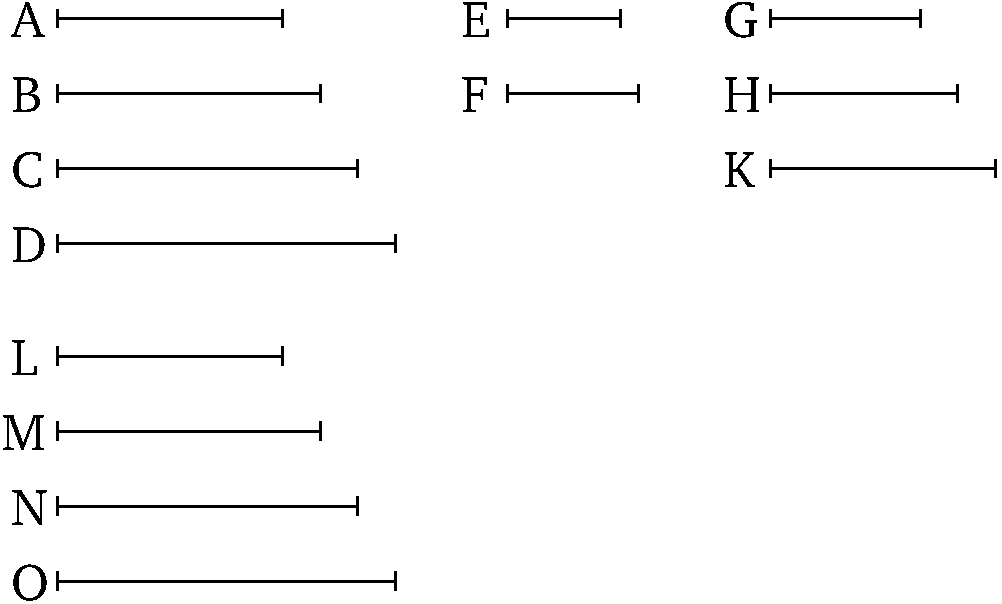
\includegraphics{Book08/fig03e.pdf}}

 Let $A$, $B$, $C$, $D$ be  any multitude whatsoever of continuously proportional
numbers (which are)  the least of those (numbers) having the same ratio as them. I say that the outermost of them, $A$ and $D$, are prime to
one another.

For let the two 
least (numbers) $E$, $F$ (which are) in the same ratio as $A$, $B$, $C$,
$D$
be taken [Prop.~7.33]. And the three
(least numbers) $G$, $H$, $K$ [Prop.~8.2].
And (so on), successively increasing by one, until the multitude of
(numbers) taken is made equal to the multitude of $A$, $B$, $C$,  $D$.
Let them be taken, and let them be $L$, $M$, $N$,  $O$.

And since $E$ and $F$ are the least of those (numbers) having the
same ratio as them they are prime to one another [Prop.~7.22]. And since  $E$, $F$ have made
 $G$,  $K$, respectively, (by) multiplying themselves [Prop.~8.2~corr.], and  have made $L$,  $O$ 
(by) multiplying  $G$, $K$, respectively,  $G$, $K$ and $L$, $O$ are thus
 also prime to one another [Prop.~7.27]. 
And since $A$, $B$, $C$, $D$ are the least of those (numbers) having
the same ratio as them, and $L$, $M$, $N$,  $O$ are also the
least (of those numbers having the same ratio as them), being in the
same ratio as $A$, $B$, $C$, $D$, and the
multitude of $A$, $B$, $C$,  $D$ is equal to the multitude
of $L$, $M$, $N$,  $O$,  thus $A$, $B$, $C$,  $D$ are
equal to  $L$, $M$, $N$,  $O$, respectively. Thus, $A$ is equal to $L$, and $D$ to $O$. And $L$ and $O$ are prime to one another. Thus,
$A$ and $D$ are also prime to one another. (Which is) the very thing it was required to show.}
\end{Parallel}

%%%%%%
% Prop 8.4
%%%%%%
\pdfbookmark[1]{Proposition 8.4}{pdf8.4}
\begin{Parallel}{}{} 
\ParallelLText{
\begin{center}
{\large \ggn{4}.}
\end{center}\vspace*{-7pt}

\gr{Λόγων δοθέντων ὁποσωνοῦν ἐν ἐλαθίστοιξ ἀριθμοῖξ ἀριθμοὺξ
εὑρεῖν ἑχῆξ ἀνάλογον ἐλαθίστουξ ἐν τοῖξ δοθεῖσι λόγοιξ.}\\

% Removed epsf size command
\centerline{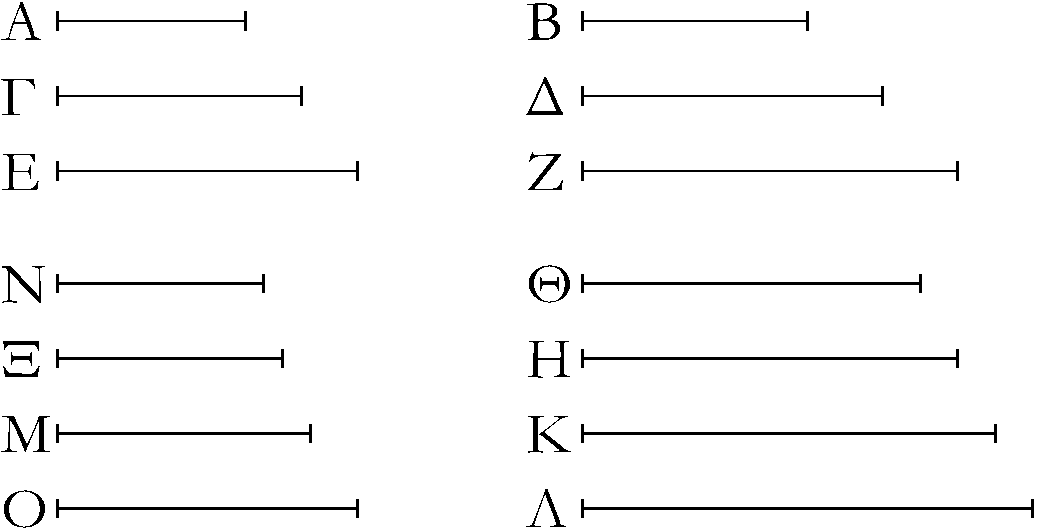
\includegraphics{Book08/fig04g.pdf}}

\gr{>'Εστωσαν οἱ δοθέντεξ λόγοι ἐν ἐλαθίστοιξ ἀριθμοῖξ <ό τε τοῦ Α
πρὸξ τὸν Β καὶ ὁ τοῦ Γ πρὸξ τὸν Δ καὶ >έτι ὁ τοῦ Ε πρὸξ
τὸν Ζ; δεῖ δὴ ἀριθμοὺξ εὑρεῖν ἑχῆξ ἀνάλογον ἐλαθίστουξ
>έν τε τῶ| τοῦ Α πρὸξ τὸν Β λόγῳ καὶ ἐν τῶ| τοῦ Γ πρὸξ
τὸν Δ καὶ >έτι τῶ| τοῦ Ε πρὸξ τὸν Ζ.}

\gr{Εἰλήφθω γὰρ ὁ ὑπὸ τῶν Β, Γ ἐλάθιστοξ μετρούμενοξ ἀριθμὸξ
ὁ Η. καὶ ὁσάκιξ μὲν ὁ Β τὸν Η μετρεῖ, τοσαυτάκιξ καὶ ὁ Α τὸν
Θ μετρείτω, ὁσάκιξ δὲ ὁ Γ τὸν Η μετρεῖ, τοσαυτάκιξ καὶ ὁ Δ τὸν Κ
μετρείτω. ὁ δὲ Ε τὸν Κ >ήτοι μετρεῖ >ὴ οὐ μετρεῖ. μετρείτω πρότερον. καὶ ὁσάκιξ ὁ Ε τὸν Κ μετρεῖ, τοσαυτάκιξ καὶ ὁ Ζ τὸν Λ μετρείτω. καὶ ἐπεὶ ἰσάκιξ ὁ Α τὸν Θ μετρεῖ καὶ ὁ Β τὸν Η, >έστιν
>άρα ὡξ ὁ Α πρὸξ τὸν Β, ο<ύτωξ ὁ Θ πρὸξ τὸν Η. διὰ τὰ α\kern -.7pt  ὐτὰ δὴ καὶ ὡξ ὁ Γ πρὸξ τὸν Δ, ο<ύτωξ ὁ Η πρὸξ τὸν Κ, καὶ >έτι ὡξ ὁ
Ε πρὸξ τὸν Ζ, ο<ύτωξ ὁ Κ πρὸξ τὸν Λ; οἱ Θ, Η, Κ, Λ >άρα ἑχῆξ ἀνάλογόν εἰσιν >έν τε τῶ| τοῦ Α πρὸξ τὸν Β καὶ ἐν τῶ| τοῦ
Γ πρὸξ τὸν Δ καὶ >έτι ἐν τῶ| τοῦ Ε πρὸξ τὸν Ζ λόγῳ. λέγω δή, <ότι
καὶ ἐλάθιστοι. εἰ γὰρ μ\kern -.7pt  ή εἰσιν οἱ Θ, Η, Κ, Λ
ἑχῆξ ἀνάλογον ἐλάθιστοι >έν τε τοῖξ τοῦ Α πρὸξ τὸν Β καὶ τοῦ
Γ πρὸξ τὸν Δ καὶ ἐν τῶ| τοῦ Ε πρὸξ τὸν Ζ λόγοιξ, >έστωσαν οἱ
Ν, Χ, Μ, Ο. καὶ ἐπεί ἐστιν ὡξ ὁ Α πρὸξ τὸν Β, ο<ύτωξ ὁ Ν
πρὸξ τὸν Χ, οἱ δὲ Α, Β ἐλάθιστοι, οἱ δὲ ἐλάθιστοι μετροῦσι τοὺξ τὸν
α\kern -.5pt  ὐτὸν λόγον >έθονταξ ἰσάκιξ <ό τε μείζων τὸν μείζονα καὶ ὁ ἐλάσσων τὸν ἐλάσσονα, τουτέστιν <ό τε ἡγούμενοξ τὸν ἡγούμενον καὶ ὁ ἑπόμενοξ τὸν ἑπόμενον, ὁ Β >άρα τὸν Χ μετρεῖ. διὰ τὰ
α\kern -.3pt  ὐτὰ δὴ καὶ ὁ Γ τὸν Χ μετρεῖ; οἱ Β, Γ >άρα τὸν Χ μετροῦσιν;
καὶ ὁ ἐλάθιστοξ >άρα ὑπὸ τῶν Β, Γ μετρούμενοξ τὸν Χ μετρήσει.
ἐλάθιστοξ δὲ ὑπὸ τῶν Β, Γ μετρεῖται ὁ Η; ὁ Η >άρα τὸν Χ μετρεῖ
ὁ μείζων τὸν ἐλάσσονα; <όπερ ἐστὶν ἀδύντατον. οὐκ >άρα >έσονταί τινεξ τῶν Θ, Η, Κ, Λ ἐλάσσονεξ ἀριθμοὶ ἑχῆξ >έν τε τῶ| τοῦ Α πρὸξ
τὸν Β καὶ τῶ| τοῦ Γ πρὸξ τὸν Δ καὶ >έτι τῶ| τοῦ Ε πρὸξ τὸν Ζ
λόγῶ|.}\\~\\~\\~\\~\\

% Removed epsf size command
\centerline{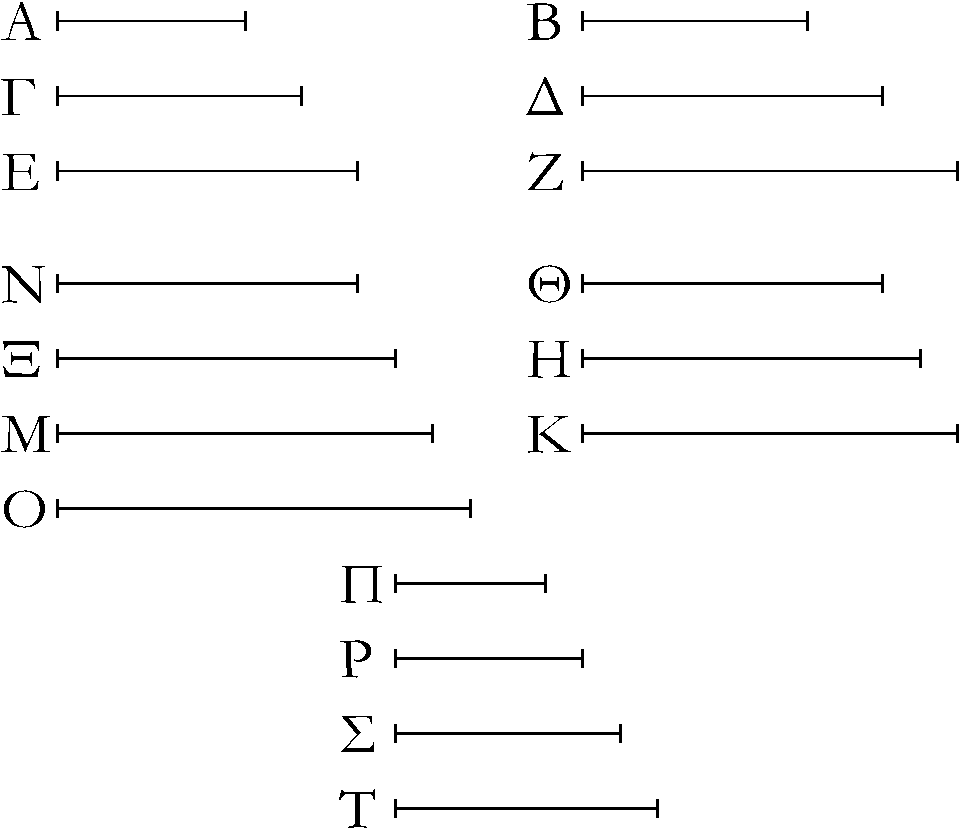
\includegraphics{Book08/fig04ag.pdf}}

\gr{μ\kern -.7pt  ὴ μετρείτω δὴ ὁ Ε τὸν Κ, καὶ εἰλήφθω ὑπὸ τῶν Ε, Κ ἐλάθιστοξ
μετρούμενοξ ἀριθμὸξ ὁ Μ. καὶ ὁσάκιξ μὲν ὁ Κ τὸν Μ
μετρεῖ, τοσαυτάκιξ καὶ ἑκάτεροξ τῶν Θ, Η ἑκάτερον τῶν Ν, Χ μετρείτω,
ὁσάακιξ δὲ ὁ Ε τὸν Μ μετρεῖ, τοσαυτάκιξ καὶ ὁ Ζ τὸν Ο μετρείτω.
ἐπεὶ ἰσάκιξ ὁ Θ τὸν Ν μετρεῖ καὶ ὁ Η τὸν Χ, >έστιν >άρα
ὡξ ὁ Θ πρὸξ τὸν Η, ο<ύτωξ ὁ Ν πρὸξ τὸν Χ. ὡξ δὲ ὁ Θ πρὸξ τὸν Η,
ο<ύτωξ ὁ Α πρὸξ τὸν Β; καὶ ὡξ >άρα ὁ Α πρὸξ τὸν Β, ο<ύτωξ
ὁ Ν πρὸξ τὸν Χ.  διὰ
τὰ α\kern -.7pt  ὐτὰ δὴ καὶ ὡξ ὁ Γ πρὸξ τὸν Δ, ο<ύτωξ ὁ Χ πρὸξ τὸν Μ. πάλιν,
ἐπεὶ ἰσάκιξ ὁ Ε  τὸν Μ μετρεῖ καὶ ὁ Ζ τὸν Ο, >έστιν >άρα
ὡξ ὁ Ε πρὸξ  τὸν Ζ, ο<ύτωξ ὁ Μ πρὸξ τὸν Ο; οἱ Ν, Χ, Μ, Ο
>άρα ἑχῆξ ἀνάλογόν εἰσιν ἐν τοῖξ τοῦ τε Α πρὸξ τὸν Β καὶ τοῦ
Γ πρὸξ  τὸν Δ καὶ >έτι τοῦ Ε πρὸξ τὸν Ζ λόγοιξ. λέγω δή, <ότι καὶ
ἐλάθιστοι ἐν τοῖξ Α Β, Γ Δ, Ε Ζ λόγοιξ. εἰ  γὰρ μ\kern -.5pt  ή, >έσονταί τινεξ τῶν Ν, Χ, Μ, Ο
ἐλάσσονεξ ἀριθμοὶ ἑχῆξ ἀνάλογον ἐν τοῖξ Α Β, Γ Δ, Ε Ζ
λόγοιξ. >έστωσαν οἱ Π, Ρ, Σ, Τ. καὶ ἐπεί ἐστιν ὡξ ὁ Π πρὸξ τὸν Ρ,
ο<ύτωξ ὁ Α πρὸξ τὸν Β, οἱ δὲ Α, Β ἐλάθιστοι, οἱ δὲ ἐλάθιστοι
μετροῦσι τοὺξ τὸν α\kern -.3pt  ὐτὸν λόγον >έθονταξ
α\kern -.7pt  ὐτοῖξ ἰσάκιξ <ό τε ἡγούμενοξ τὸν ἡγούμενον καὶ ὁ ἑπόμενοξ
τὸν ἑπόμενον, ὁ Β >άρα τὸν Ρ μετρεῖ. διὰ τὰ α\kern -.7pt  ὐτὰ δὴ καὶ ὁ Γ τὸν
Ρ μετρεῖ; οἱ Β, Γ >άρα τὸν Ρ μετροῦσιν. καὶ ὁ ἐλάθιστοξ >άρα ὑπὸ
τῶν Β, Γ μετούμενοξ τὸν Ρ μετρήσει. ἐλάθιστοξ δὲ ὑπὸ τῶν
Β, Γ μετρούμενοξ ἐστιν ὁ Η; ὁ Η >άρα τὸν Ρ μετρεῖ.
καί ἐστιν ὡξ ὁ Η πρὸξ τὸν  Ρ, ο<ύτωξ ὁ Κ πρὸξ τὸν Σ; καὶ
ὁ Κ >άρα τὸν Σ μετρεῖ. μετρεῖ δὲ καὶ ὁ Ε τὸν Σ; οἱ Ε, Κ
>άρα τὸν Σ
μετροῦσιν. καὶ ὁ ἐλάθιστοξ >άρα ὑπὸ τῶν
Ε, Κ μετρούμενοξ τὸν Σ μετρήσει. ἐλάθιστοξ δὲ ὑπὸ τῶν Ε, Κ
μετρούμενόξ ἐστιν ὁ Μ; ὁ Μ >άρα τὸν Σ μετρεῖ ὁ μείζων
τὸν ἐλάσσονα; <όπερ ἐστὶν ἀδύνατον. οὐκ >άρα >έσονταί τινεξ τῶν
Ν, Χ, Μ, Ο ἐλάσσονεξ ἀριθμοὶ ἑχῆξ ἀνάλογον >έν τε τοῖξ
τοῦ Α πρὸξ τὸν Β καὶ τοῦ Γ πρὸξ τὸν Δ καὶ >έτι τοῦ Ε πρὸξ τὸν
Ζ λόγοιξ; οἱ Ν, Χ, Μ, Ο >άρα ἑχῆξ ἀνάλογον ἐλάθιστοί εἰσιν
ἐν τοῖξ Α Β, Γ Δ, Ε Ζ λόγοιξ; <όπερ >έδει δεῖχαι.}}

\ParallelRText{
\begin{center}
{\large Proposition 4}
\end{center}

For any multitude whatsoever of given ratios, (expressed) in the least numbers, to find the least numbers continuously proportional 
in these given ratios.

% Removed epsf size command
\centerline{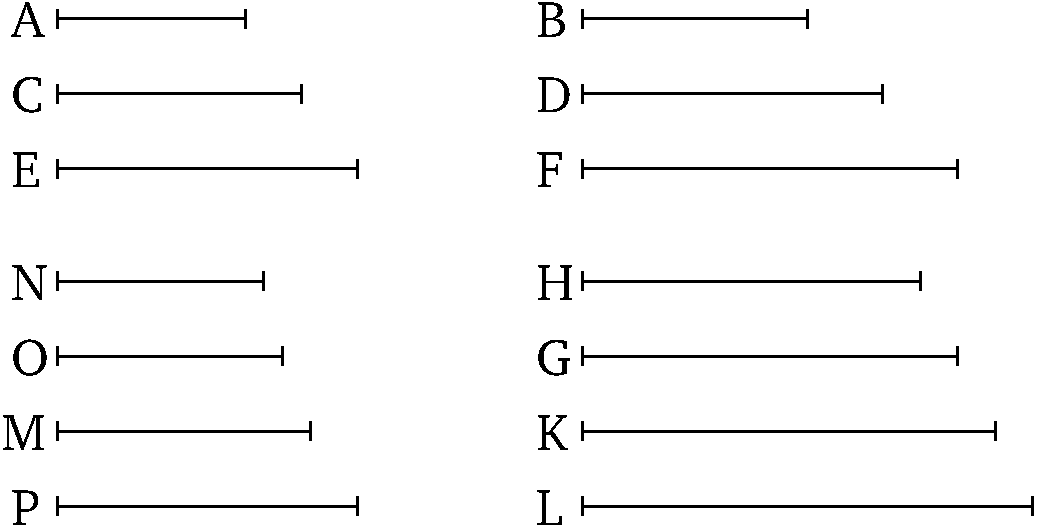
\includegraphics{Book08/fig04e.pdf}}

Let the given ratios, (expressed) in the least numbers, be the (ratios) of
$A$ to $B$, and of $C$ to $D$, and, further,  of $E$ to $F$. So it is
required to find the least numbers continuously proportional  in the
ratio of $A$ to $B$, and  of $C$ to $B$, and, further,
 of $E$ to $F$.
 
For let the least number, $G$,  measured by (both) $B$ and $C$ have
be taken [Prop.~7.34]. And as many times
as $B$ measures $G$, so many times let $A$ also measure $H$.
And as many times as $C$ measures $G$, so many times let
$D$ also measure $K$. And $E$ either measures, or does not measure, $K$.
Let it, first of all, measure ($K$). And as many times as $E$ measures
$K$, so many times let $F$ also measure $L$. And since $A$
measures $H$ the same number of times that $B$ also (measures) $G$, thus as $A$ is to $B$, so $H$ (is) to $G$ [Def.~7.20, Prop.~7.13].
And so, for the same (reasons), as $C$ (is) to $D$, so
$G$ (is) to $K$, and, further, as $E$ (is) to $F$, so $K$ (is) to $L$.
Thus, $H$, $G$, $K$, $L$ are continuously proportional in the ratio
of $A$ to $B$, and of $C$ to $D$, and, further,  of $E$ to $F$. So I say that (they are) also the least
(numbers continuously proportional in these ratios). For if
$H$, $G$, $K$, $L$ are not the least numbers continuously proportional
 in the ratios of $A$ to $B$, and of $C$ to $D$, and of
$E$ to $F$, let $N$, $O$, $M$, $P$ be (the least such numbers). 
And since as $A$ is to $B$, so $N$ (is) to $O$, and $A$ and $B$ are the
least (numbers which have the same ratio as them), and the least (numbers) measure those (numbers)
having the same ratio (as them) an equal number of times, the greater (measuring) the greater, and the lesser the lesser---that is to say, the leading (measuring) the leading, and the
following the following [Prop.~7.20], $B$ thus
measures $O$. So, for the same (reasons), $C$ also measures $O$. Thus,
$B$ and $C$ (both) measure $O$. Thus, the least number measured by
(both) $B$ and $C$ will also measure $O$ [Prop.~7.35]. And $G$ (is) the least number measured by (both) $B$ and $C$. Thus, $G$ measures $O$, the greater
(measuring) the lesser. The very thing is impossible. Thus, there
cannot be any numbers less than $H$, $G$, $K$, $L$ 
(which are) continuously (proportional) in the ratio of $A$ to $B$, and of $C$ to $D$, and, further, of $E$ to $F$.

% Removed epsf size command
\centerline{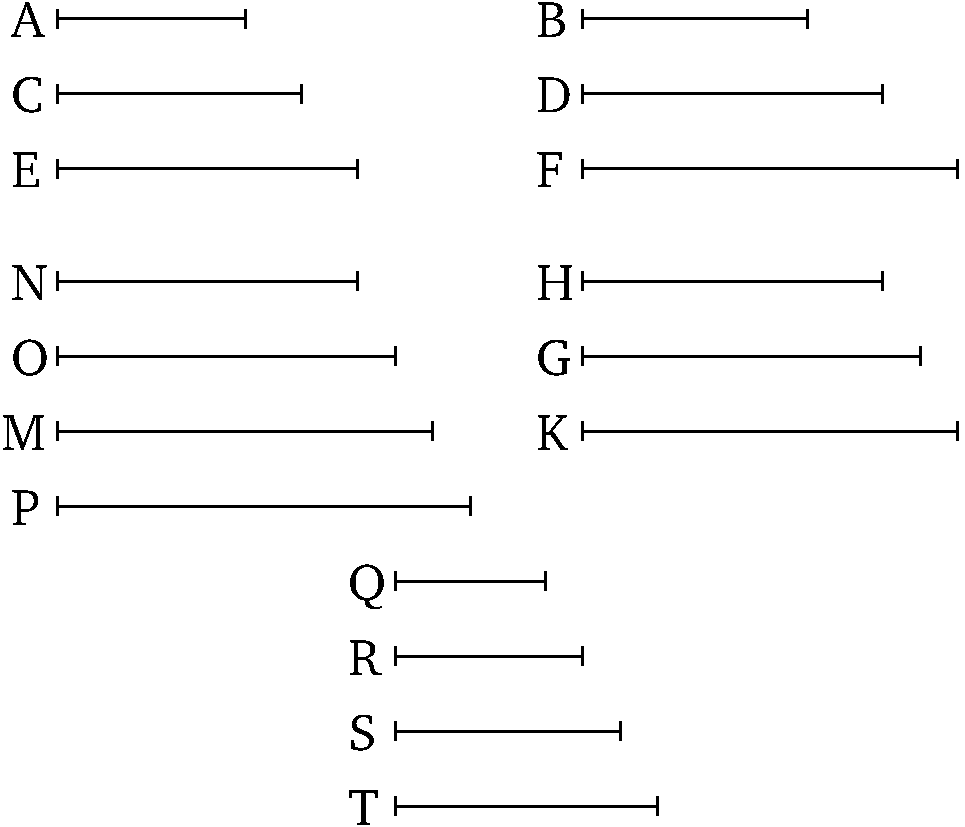
\includegraphics{Book08/fig04ae.pdf}}

So let $E$ not measure $K$. And let the least number, $M$, measured by 
(both) $E$ and $K$ be taken [Prop.~7.34]. And as
many times as $K$ measures $M$, so many times let  $H$, $G$
also measure  $N$, $O$, respectively.  And as many times as $E$ measures $M$,
so many times let $F$ also measure $P$. Since $H$ measures $N$ the same
number of times as $G$
(measures) $O$, thus as $H$ is to $G$, so
$N$ (is) to $O$ [Def.~7.20, Prop.~7.13]. And as $H$ (is) to $G$, so $A$ (is)
to $B$. And thus as $A$ (is) to $B$, so $N$ (is) to $O$. And so, for the
same (reasons),  as $C$ (is) to $D$, so $O$ (is) to $M$. Again, since
$E$ measures $M$ the same number of times as $F$ (measures) $P$,
thus as $E$ is to $F$, so $M$ (is) to $P$ [Def.~7.20, Prop.~7.13]. Thus, $N$, $O$, $M$, $P$ are continuously proportional in the ratios of $A$ to $B$, and of $C$ to $D$, and,
further, of $E$ to $F$. So I say that (they are) also the least (numbers)
in the ratios of $A$ $B$, $C$ $D$, $E$ $F$.
For if not, then there will be some numbers less than $N$, $O$, $M$, $P$
(which are) continuously proportional in the ratios of $A$ $B$, $C$ $D$,
$E$ $F$. Let them be $Q$, $R$, $S$, $T$.
And since as $Q$ is to $R$, so $A$ (is) to $B$, and $A$ and $B$ (are) the
least (numbers having the same ratio as them), and the least (numbers) measure those
(numbers) having the same ratio as them an equal number of times, the leading (measuring) the leading, and the following the following [Prop.~7.20], $B$ thus measures $R$. So, for the
same (reasons), $C$ also measures $R$.  Thus, $B$ and $C$ (both)
measure $R$. Thus, the least (number) measured by (both) $B$ and $C$ will
also measure $R$ [Prop.~7.35]. And $G$ is the
least number measured by (both) $B$ and $C$. Thus, $G$ measures $R$.
And as $G$ is to $R$, so $K$ (is) to $S$. Thus, $K$ also measures $S$
[Def.~7.20]. And $E$ also measures $S$ [Prop.~7.20]. Thus, $E$ and $K$ (both) measure
$S$. Thus, the least (number) measured by (both) $E$ and $K$ will also
measure $S$   [Prop.~7.35]. And $M$  is the least (number) measured by (both)
$E$ and $K$. Thus, $M$ measures $S$, the greater (measuring) the lesser. The very thing is impossible.
Thus there cannot be any numbers less than $N$, $O$, $M$, $P$ (which
are) continuously proportional in the ratios of $A$ to $B$, and of
$C$ to $D$, and, further, of $E$ to $F$. Thus, $N$, $O$, $M$, $P$
are the least (numbers) continuously proportional in the ratios
of $A$ $B$, $C$ $D$, $E$ $F$. (Which is) the very thing it
was required to show.}
\end{Parallel}

%%%%%%
% Prop 8.5
%%%%%%
\pdfbookmark[1]{Proposition 8.5}{pdf8.5}
\begin{Parallel}{}{} 
\ParallelLText{
\begin{center}
{\large \ggn{5}.}
\end{center}\vspace*{-7pt}

\gr{Οἱ ἐπίπεδοι ἀριθμοὶ πρὸξ ἀλλήλουξ λόγον >έθουσι τὸν συγκείμενον
ἐκ τῶν πλευρῶν.}

% Removed epsf size command
\centerline{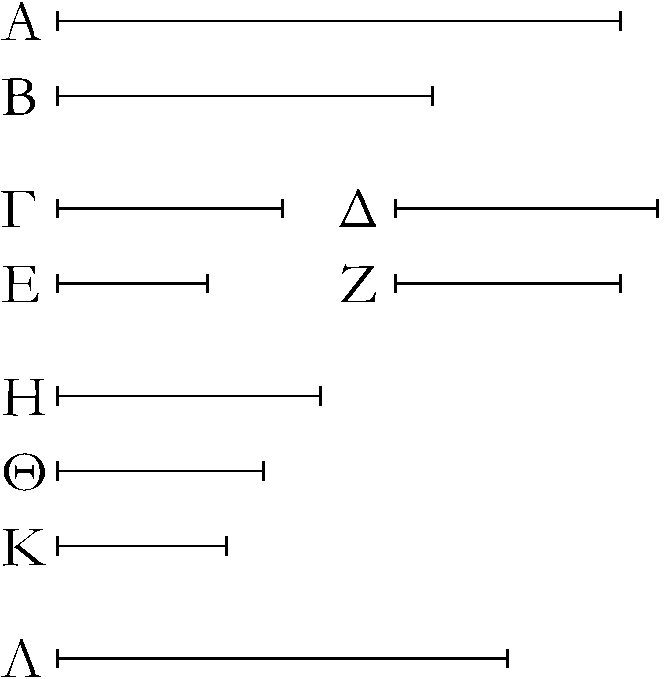
\includegraphics{Book08/fig05g.pdf}}

\gr{>'Εστωσαν ἐπίπεδοι ἀριθμοὶ οἱ Α, Β, καὶ τοῦ μὲν Α πλευραὶ
>έστωσαν οἱ Γ, Δ ἀριθμοί, τοῦ δὲ Β οἱ Ε, Ζ; λέγω, <ότι ὁ Α
πρὸξ τὸν Β λόγον >έθει τὸν συγκείμενον ἐκ τῶν πλευρῶν.}

\gr{Λόγων γὰρ δοθέντων τοῦ τε <ὸν >έθει ὁ Γ πρὸξ τὸν Ε καὶ
ὁ Δ πρὸξ τὸν Ζ εἰλήφθωσαν ἀριθμοὶ ἑχῆξ ἐλάθιστοι ἐν τοῖξ
Γ Ε, Δ Ζ λόγοιξ, οἱ Η, Θ, Κ, <ώστε ε>ῖναι ὡξ μὲν τὸν Γ πρὸξ τὸν Ε,
ο<ύτωξ τὸν Η πρὸξ τὸν Θ, ὡξ δὲ τὸν Δ πρὸξ τὸν Ζ, ο<ύτωξ
τὸν Θ πρὸξ τὸν Κ. καὶ ὁ Δ τὸν Ε πολλαπλασιάσαξ τὸν Λ ποιείτω.}

\gr{Καὶ ἐπεὶ ὁ Δ τὸν μὲν Γ πολλαπλασιάσαξ τὸν Α πεποίηκεν, τὸν
δὲ Ε πολλαπλασιάσαξ τὸν Λ πεποίηκεν, >έστιν >άρα ὡξ ὁ Γ πρὸξ
τὸν Ε, ο<ύτωξ ὁ Α πρὸξ τὸν Λ. ὡξ δὲ ὁ Γ πρὸξ τὸν Ε, ο<ύτωξ
ὁ Η πρὸξ τὸν Θ; καὶ ὡξ >άρα ὁ Η πρὸξ τὸν Θ, ο<ύτωξ ὁ Α πρὸξ
τὸν Λ. πάλιν, ἐπεὶ ὁ Ε τὸν Δ πολλαπλασιάσαξ τὸν Λ πεποίηκεν,
ἀλλὰ μ\kern -.7pt  ὴν καὶ τὸν Ζ πολλαπλασιάσαξ τὸν Β 
πεποίηκεν, >έστιν
>άρα ὡξ ὁ Δ πρὸξ τὸν Ζ, ο<ύτωξ ὁ Λ πρὸξ τὸν Β. ἀλλ> ὡξ ὁ Δ
πρὸξ τὸν Ζ, ο<ύτωξ ὁ Θ πρὸξ τὸν Κ; καὶ ὡξ >άρα ὁ Θ πρὸξ τὸν Κ,
ο<ύτωξ ὁ Λ πρὸξ τὸν Β. ἐδείθθη δὲ καὶ ὡξ ὁ Η πρὸξ τὸν Θ, ο<ύτωξ
ὁ Α πρὸξ τὸν Λ; δι> >ίσου >άρα ἐστὶν ὡξ ὁ Η πρὸξ τὸν Κ, [ο<ύτωξ]
ὁ Α πρὸξ τὸν Β. ὁ δὲ Η πρὸξ τὸν Κ λόγον >έθει τὸν συγκείμενον
ἐκ τῶν πλευρῶν; καὶ ὁ Α >άρα πρὸξ τὸν Β λόγον >έθει τὸν συγκείμενον ἐκ τῶν πλευρῶν; <όπερ >έδει δεῖχαι.}}

\ParallelRText{
\begin{center}
{\large Proposition 5}
\end{center}

Plane numbers have to one another the ratio compoun\-ded$^\dag$ out of (the ratios of)
 their sides.
 
 % Removed epsf size command
\centerline{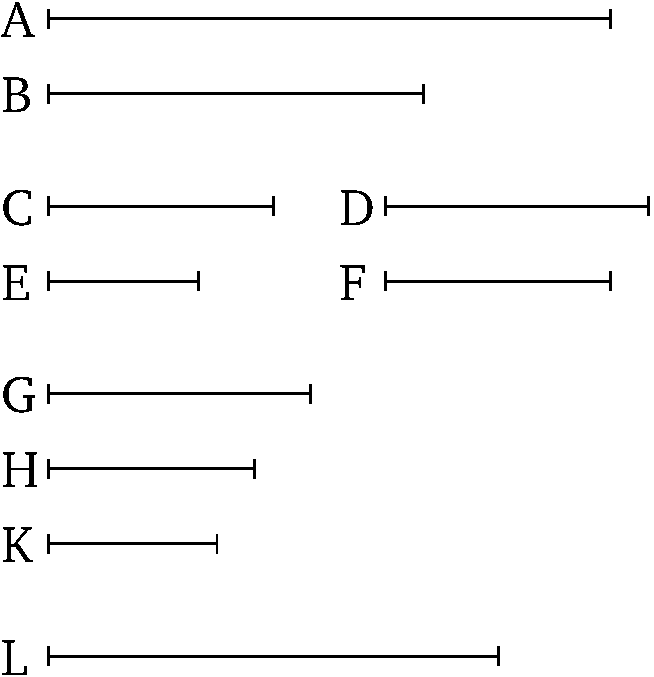
\includegraphics{Book08/fig05e.pdf}}

Let $A$ and $B$ be plane numbers, and let the numbers $C$, $D$ be the
sides of $A$, and (the numbers) $E$, $F$ (the sides) of $B$. I say that $A$ has to $B$ the ratio compounded out of (the ratios of)  their sides.

For given the ratios which $C$ has to $E$, and $D$ (has) to $F$, let the least numbers, $G$, $H$, $K$, continuously proportional in the
ratios $C$ $E$, $D$ $F$ be taken [Prop.~8.4], so that as $C$ is to $E$, so
$G$ (is) to $H$, and as $D$ (is) to $F$, so $H$ (is) to $K$. And let $D$ make $L$ (by) multiplying $E$. 

And since $D$ has made $A$ (by) multiplying $C$, and has made $L$ (by)
multiplying $E$, thus as $C$ is to  $E$, so $A$ (is) to $L$ [Prop.~7.17]. And as $C$ (is) to $E$, so $G$ (is) to
$H$. And thus as $G$ (is) to $H$, so $A$ (is) to $L$. Again, since
$E$ has made $L$ (by) multiplying $D$ [Prop.~7.16],
but, in fact, has also made $B$ (by) multiplying $F$, thus as $D$ is to 
$F$, so $L$ (is) to $B$  [Prop.~7.17]. But,
as $D$ (is) to $F$, so $H$ (is) to $K$.  And thus as $H$ (is) to $K$, so
$L$ (is) to $B$. And it was also shown that as $G$ (is) to $H$, so $A$ (is)
to $L$. Thus, via equality, as $G$ is to $K$, [so] $A$ (is) to $B$ [Prop.~7.14]. 
And $G$ has to $K$ the ratio compounded out of (the ratios
of) the sides (of $A$ and $B$). Thus, $A$ also has to $B$ the ratio
compounded out of (the ratios of) the sides (of $A$ and $B$). (Which is)
the very thing it was required to show.}
\end{Parallel}
{\footnotesize\noindent$^\dag$ {\rm i.e.}, multiplied.}

%%%%%%
% Prop 8.6
%%%%%%
\pdfbookmark[1]{Proposition 8.6}{pdf8.6}
\begin{Parallel}{}{} 
\ParallelLText{
\begin{center}
{\large \ggn{6}.}
\end{center}\vspace*{-7pt}

\gr{Ἐὰν >ῶσιν ὁποσοιοῦν ἀριθμοὶ ἑχῆξ ἀνάλογον, ὁ δὲ πρῶτοξ
τὸν δεύτερον μ\kern -.7pt  ὴ μετρῆ|, οὐδὲ >άλλοξ οὐδεὶξ οὐδένα μετρήσει.}

\gr{>'Εστωσαν ὁποσοιοῦν ἀριθμοὶ ἑχῆξ ἀνάλογον οἱ Α, Β, Γ, Δ, Ε,
ὁ δὲ Α τὸν Β μ\kern -.7pt  ὴ μετρείτω; λέγω, <ότι οὐδὲ >άλλοξ οὐδεὶξ
οὐδένα μετρήσει.}\\~\\

% Removed epsf size command
\centerline{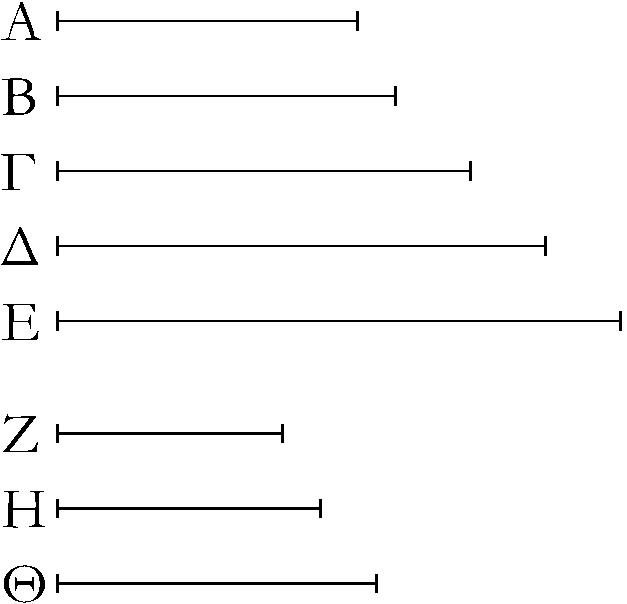
\includegraphics{Book08/fig06g.pdf}}

\gr{<'Οτι μὲν ο>ῦν οἱ Α, Β, Γ, Δ, Ε ἑχῆξ ἀλλήλουξ οὐ μετροῦσιν,
φανερόν; οὐδὲ γὰρ ὁ Α τὸν Β μετρεῖ. λέγω δή, <ότι οὐδὲ >άλλοξ
οὐδεὶξ οὐδένα μετρήσει. εἰ γὰρ δυνατόν, μετρείτω ὁ Α τὸν Γ.
καὶ <όσοι εἰσὶν οἱ Α, Β, Γ, τοσοῦτοι εἰλήφθωσαν ἐλάθιστοι
ἀριθμοὶ τῶν τὸν α\kern -.7pt  ὐτὸν λόγον ἐθόντων τοῖξ Α, Β, Γ οἱ Ζ, Η,
Θ. καὶ ἐπεὶ οἱ Ζ, Η, Θ ἐν τῶ| α\kern -.7pt  ὐτῶ| λόγῳ εἰσὶ τοῖξ Α, Β, Γ,
καί ἐστιν >ίσον τὸ πλῆθοξ τῶν Α, Β, Γ τῶ| πλήθει τῶν Ζ, Η, Θ, δι>
>ίσου >άρα ἐστὶν ὡξ ὁ Α πρὸξ τὸν Γ, ο<ύτωξ ὁ Ζ πρὸξ τὸν
Θ. καὶ ἐπεί ἐστιν ὡξ ὁ Α πρὸξ τὸν Β, ο<ύτωξ ὁ Ζ πρὸξ τὸν Η,
οὐ μετρεῖ δὲ ὁ Α τὸν Β, οὐ μετρεῖ >άρα οὐδὲ ὁ Ζ τὸν 
Η; οὐκ >άρα μονάξ ἐστιν ὁ Ζ; ἡ γὰρ μονὰξ πάντα ἀριθμὸν
μετρεῖ. καί εἰσιν οἱ Ζ, Θ πρῶτοι πρὸξ ἀλλήλουξ [οὐδὲ ὁ Ζ
>άρα τὸν Θ μετρεῖ]. καί ἐστιν ὡξ ὁ Ζ πρὸξ τὸν Θ, ο<ύτωξ
ὁ Α πρὸξ τὸν Γ; οὐδὲ ὁ Α >άρα τὸν Γ μετρεῖ. ὁμοίωξ
δὴ δείχομεν, <ότι οὐδὲ >άλλοξ οὐδεὶξ οὐδένα μετρήσει;
<όπερ >έδει δεῖχαι.}}

\ParallelRText{
\begin{center}
{\large Proposition 6}
\end{center}

If there are any multitude whatsoever of continuously
proportional numbers, and the first does not measure the second, then no other (number) will
 measure any other (number) either.
 
 Let $A$, $B$, $C$, $D$, $E$ be any multitude whatsoever of continuously
 proportional numbers, and let $A$ not measure $B$.  I say that 
 no other (number) will measure any other (number) either.
 
 % Removed epsf size command
\centerline{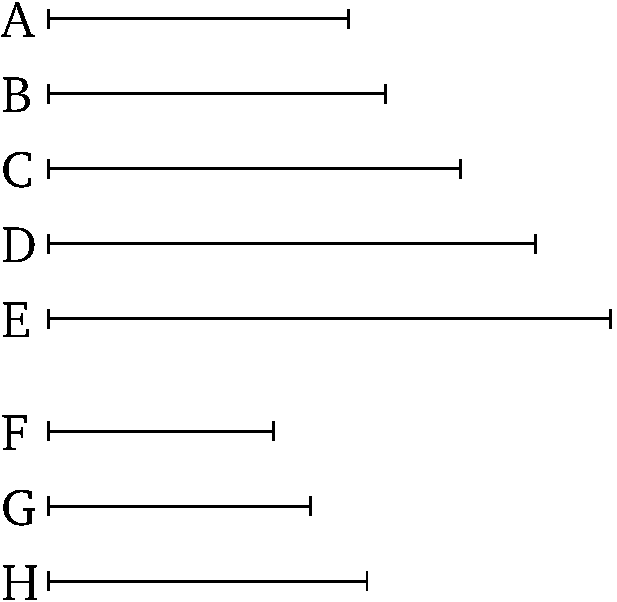
\includegraphics{Book08/fig06e.pdf}}

 
 Now, (it is) clear that $A$, $B$, $C$, $D$, $E$ do not successively measure
 one another. For $A$ does not even measure $B$. So I say that  
 no other (number) will measure any other (number) either. For, if possible, let $A$ measure
 $C$. And as many (numbers) as  are $A$, $B$, $C$, let  so many of the least numbers,
 $F$, $G$, $H$, be taken of those (numbers) having the same ratio as $A$, $B$, $C$ [Prop.~7.33]. And since $F$, $G$, $H$ are in the same ratio as $A$, $B$, $C$, and the multitude of
 $A$, $B$, $C$ is equal to the multitude of $F$, $G$, $H$, thus, via
 equality, as $A$ is to $C$, so $F$ (is) to $H$ [Prop.~7.14]. And since as $A$ is to $B$, so $F$ (is) to $G$, and $A$ does not measure $B$, $F$ does not measure $G$ either
 [Def.~7.20]. Thus, $F$ is not a unit. For a unit measures all numbers. And $F$ and $H$ are prime to one another [Prop.~8.3] [and thus $F$ does not measure $H$].
 And as $F$ is to $H$, so $A$ (is) to $C$. And thus $A$ does not measure
 $C$ either [Def.~7.20]. So, similarly, we can show
 that no other (number) can measure any other (number) either.
 (Which is) the very thing it was required to show.}
\end{Parallel}

%%%%%%
% Prop 8.7
%%%%%%
\pdfbookmark[1]{Proposition 8.7}{pdf8.7}
\begin{Parallel}{}{} 
\ParallelLText{
\begin{center}
{\large \ggn{7}.}
\end{center}\vspace*{-7pt}

\gr{Ἐὰν >ῶσιν ὁποσοιοῦν ἀριθμοὶ [ἑχῆξ] ἀνάλογον,
ὁ δὲ πρῶτοξ τὸν >έσθατον μετρῆ|, καὶ τὸν δεύτερον μετρήσει.}\\

% Removed epsf size command
\centerline{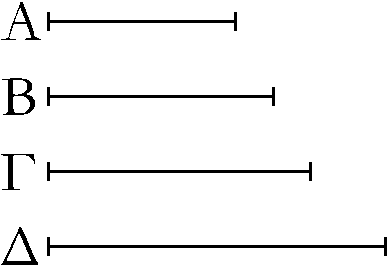
\includegraphics{Book08/fig07g.pdf}}

\gr{>'Εστωσαν ὁποσοιοῦν ἀριθμοὶ ἑχῆξ ἀνάλογον οἱ Α, Β, Γ, Δ,
ὁ δὲ Α τὸν Δ μετρείτω; λέγω, <ότι καὶ ὁ Α τὸν Β μετρεῖ.}

\gr{Εἰ γὰρ οὐ μετρεῖ ὁ Α τὸν Β, οὐδὲ >άλλοξ οὐδεὶξ οὐδένα
μετρήσει; μετρεῖ δὲ ὁ Α τὸν Δ. μετρεῖ >άρα καὶ ὁ Α τὸν Β;
<όπερ >έδει δεῖχαι.}}

\ParallelRText{
\begin{center}
{\large Proposition 7}
\end{center}

If there are any multitude whatsoever of [continuously] proportional numbers, and the first measures the last, then (the first)
will also measure the second.

% Removed epsf size command
\centerline{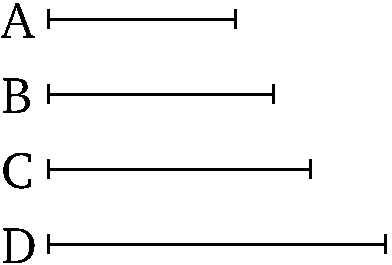
\includegraphics{Book08/fig07e.pdf}}

Let $A$, $B$, $C$, $D$ be any number whatsoever of continuously proportional numbers. And let $A$ measure $D$. I say that $A$ also measures $B$.

For if $A$ does not measure $B$ then no other (number) will measure
any other (number) either [Prop.~8.6]. 
But $A$ measures $D$. Thus, $A$ also measures $B$. (Which is) the
very thing it was required to show.}
\end{Parallel}

%%%%%%
% Prop 8.8
%%%%%%
\pdfbookmark[1]{Proposition 8.8}{pdf8.8}
\begin{Parallel}{}{} 
\ParallelLText{
\begin{center}
{\large \ggn{8}.}
\end{center}\vspace*{-7pt}

\gr{Ἐὰν  δύο ἀριθμῶν μεταχὺ κατὰ τὸ συνεθὲξ ἀνάλογον ἐμπίπτωσιν
ἀριθμοί, <όσοι εἰξ α\kern -.7pt  ὐτοὺξ μεταχὺ κατὰ τὸ συνεθὲξ ἀνόλογον ἐμπίπτουσιν ἀριθμοί, τοσοῦτοι καὶ εἰξ τοὺξ τὸν α\kern -.7pt  ὐτὸν λόγον
>έθονταξ [α\kern -.5pt  ὐτοῖξ] μεταχὺ κατὰ τὸ συνὲθεξ ἀνάλογον ἐμπεσοῦνται}

% Removed epsf size command
\centerline{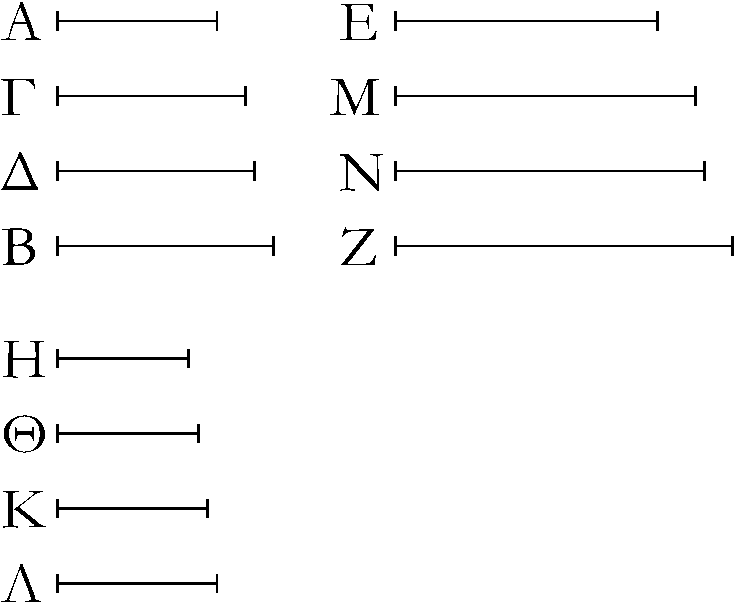
\includegraphics{Book08/fig08g.pdf}}

\gr{Δύο γὰρ ἀριθμῶν τῶν Α, Β μεταχὺ κατὰ τὸ συνεθὲξ ἀνάλογον
ἐμπιπτέτωσαν ἀριθμοὶ οἱ Γ, Δ,  καὶ πεποιήσθω ὡξ ὁ Α πρὸξ
τὸν Β, ο<ύτωξ ὁ Ε πρὸξ τὸν Ζ; λέγω, <ότι <όσοι εἰξ τοὺξ Α, Β
μεταχὺ κατὰ τὸ συνεθὲξ ἀνάλογον ἐμπεπτώκασιν ἀριθμοί,
τοσοῦτοι καὶ εἰξ τοὺξ Ε, Ζ μεταχὺ κατὰ τὸ συνεθὲξ ἀνάλογον
ἐμπεσοῦνται.}

\gr{<'Οσοι γάρ εἰσι τῶ| πλήθει οἱ Α, Β, Γ, Δ, τοσοῦτοι εἰλήφθωσαν
ἐλάθιστοι ἀριθμοὶ τῶν τὸν α\kern -.7pt  ὐτὸν λόγον ἐθόντων τοῖξ
Α, Γ, Δ, Β οἱ Η, Θ, Κ, Λ; οἱ >άρα >άκροι α\kern -.7pt  ὐτῶν οἱ Η, Λ πρῶτοι πρὸξ
ἀλλήλουξ εἰσίν. καὶ ἐπεὶ οἱ Α, Γ, Δ, Β τοῖξ Η, Θ, Κ, Λ ἐν τῶ| α\kern -.5pt  ὐτῶ| λόγῳ εἰσίν, καί ἐστιν >ίσον τὸ πλῆθοξ τῶν
Α, Γ, Δ, Β τῶ| πλήθει τῶν Η, Θ, Κ, Λ, δι> >ίσου >άρα ἐστὶν
ὡξ ὁ Α πρὸξ τὸν Β, ο<ύτωξ ὁ Η πρὸξ τὸν Λ. ὡξ δὲ ὁ Α
πρὸξ τὸν Β, ο<ύτωξ ὁ Ε πρὸξ τὸν Ζ; καὶ ὡξ >άρα ὁ Η πρὸξ τὸν Λ,
ο<ύτωξ ὁ Ε πρὸξ τὸν Ζ. οἱ δὲ Η, Λ πρῶτοι, οἱ δὲ πρῶτοι καὶ
ἐλάθιστοι, οἱ δὲ ἐλάθιστοι
ἀριθμοὶ μετροῦσι τοὺξ τὸν α\kern -.3pt  ὐτὸν λόγον >έθονταξ ἰσάκιξ <ό τε μείζων τὸν μείζονα καὶ ὁ ἐλάσσων τὸν ἐλάσσονα, τουτέστιν <ό τε
ἡγούμενοξ τὸν ἡγούμενον καὶ ὁ ἑπόμενοξ τὸν  ἑπόμενον.
ἰσάκιξ >άρα ὁ Η τὸν Ε μετρεῖ καὶ ὁ Λ τὸν Ζ. ὁσάκιξ δὴ ὁ Η
τὸν Ε μετρεῖ, τοσαυτάκιξ καὶ ἑκάτεροξ τῶν Θ, Κ ἑκάτερον τῶν
Μ, Ν μετρείτω; οἱ Η, Θ, Κ, Λ
>άρα τοὺξ Ε, Μ, Ν, Ζ ἰσάκιξ μετροῦσιν. οἱ Η, Θ, Κ, Λ
>άρα τοῖξ Ε, Μ, Ν, Ζ ἐν τῶ| α\kern -.7pt  ὐτῶ| λόγῳ εἰσίν. ἀλλὰ οἱ 
Η, Θ, Κ, Λ τοῖξ Α, Γ, Δ, Β ἐν τῶ| α\kern -.7pt  ὐτῶ| λόγῳ εἰσίν; καὶ
οἱ Α, Γ,  Δ, Β >άρα τοῖξ Ε, Μ, Ν, Ζ ἐν τῶ| α\kern -.7pt  ὐτῶ| λόγῳ
εἰσίν. οἱ δὲ Α, Γ, Δ, Β ἑχῆξ ἀνάλογόν
εἰσιν; καὶ οἱ Ε, Μ, Ν, Ζ  >άρα ἑχῆξ ἀνάλογόν εἰσιν.
<όσοι >άρα εἰξ τοὺξ Α, Β μεταχὺ κατὰ τὸ συνεθὲξ ἀνάλογον
ἐμπεπτώκασιν ἀριθμοί, τοσοῦτοι καὶ εἰξ τοὺξ
Ε, Ζ μεταχὺ κατὰ τὸ συνεθὲξ ἀνάλογον ἐμπεπτώκασιν
ἀριθμοί; <όπερ >έδει δεῖχαι.}}

\ParallelRText{
\begin{center}
{\large Proposition 8}
\end{center}

If between two numbers there fall (some) numbers in continued proportion then, as many  numbers as fall in between them in continued proportion, so many (numbers)  will also fall in between (any two numbers) having the same ratio [as them] in continued  proportion.

% Removed epsf size command
\centerline{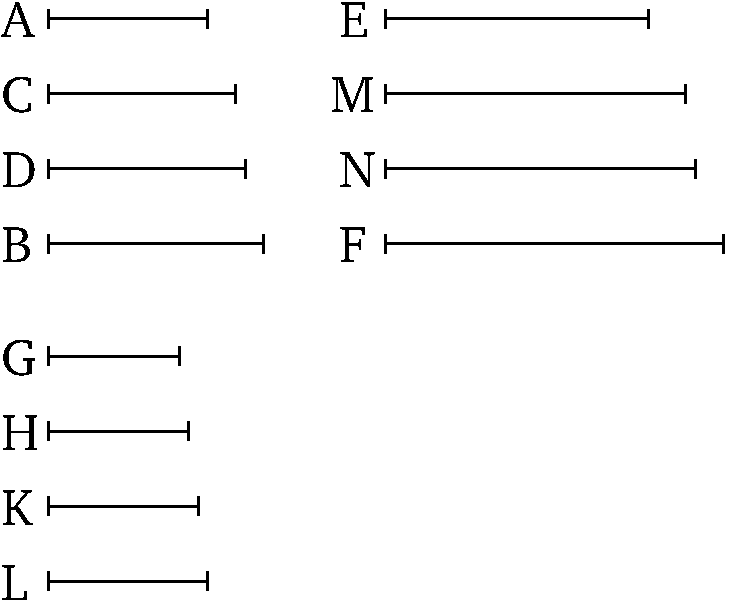
\includegraphics{Book08/fig08e.pdf}}

For let the numbers, $C$ and $D$,
 fall between two numbers, $A$ and $B$, in continued proportion, and let it be contrived
(that) as $A$ (is) to $B$, so $E$ (is) to $F$. I say that, as many numbers  as have fallen in between $A$ and $B$ in continued proportion, so many (numbers)  will also fall in between $E$ and $F$ in continued proportion.

For as many  as $A$, $B$, $C$, $D$ are in multitude, let so many
of the least numbers, $G$, $H$, $K$, $L$, having the
same ratio as $A$, $B$, $C$, $D$, be taken [Prop.~7.33]. Thus, the outermost of them, $G$ and
$L$, are prime to one another [Prop.~8.3].
And since $A$, $B$, $C$, $D$ are in the same ratio as $G$, $H$, $K$, $L$,
and the multitude of $A$, $B$, $C$, $D$ is equal to the
multitude of $G$, $H$, $K$, $L$, thus, via equality, as $A$ is to $B$,
so $G$ (is) to $L$ [Prop.~7.14].
And as $A$ (is) to $B$, so $E$ (is) to $F$. And thus as $G$ (is) to $L$,
so $E$ (is) to $F$. And $G$ and $L$ (are) prime (to one another). And (numbers) prime (to one another are) also the least (numbers having the same ratio as them) [Prop.~7.21]. And the least numbers measure
those (numbers) having the same ratio (as them) an equal number of times, the greater (measuring) the greater, and the lesser the lesser---that is to say, the leading (measuring) the leading, and the following the following [Prop.~7.20]. Thus, $G$ measures $E$ the same
number of times as $L$ (measures) $F$. So as many times as $G$ measures $E$, so many times let $H$, $K$ also measure  $M$, $N$, respectively.
Thus, $G$, $H$, $K$, $L$  measure $E$, $M$, $N$, $F$ (respectively) an equal
number of times. Thus, $G$, $H$, $K$, $L$ are in the same
ratio as $E$, $M$, $N$, $F$ [Def.~7.20]. But,
$G$, $H$, $K$, $L$ are in the same ratio as $A$, $C$, $D$, $B$. 
Thus, $A$, $C$, $D$, $B$ are also in the same ratio as $E$, $M$, $N$, $F$.
And $A$, $C$, $D$, $B$ are continuously proportional. Thus, $E$, $M$, 
$N$, $F$  are also continuously proportional. Thus, as many numbers  as have fallen in between $A$ and $B$ in
continued proportion, so many
numbers  have also fallen in between $E$ and $F$ in continued proportion.
(Which is) the very thing it was required to show.}
\end{Parallel}

%%%%%%
% Prop 8.9
%%%%%%
\pdfbookmark[1]{Proposition 8.9}{pdf8.9}
\begin{Parallel}{}{} 
\ParallelLText{
\begin{center}
{\large \ggn{9}.}
\end{center}\vspace*{-7pt}

\gr{Ἐὰν δύο ἀριθμοὶ πρῶτοι πρὸξ ἀλλήλουξ >ῶσιν, καὶ εἰξ
α\kern -.7pt  ὐτοὺξ μεταχὺ κατὰ τὸ συνεθὲξ ἀνάλογον ἐμπίπτωσιν
ἀριθμοί, <όσοι εἰξ α\kern -.7pt  ὐτοὺξ μεταχὺ κατὰ τὸ συνεθὲξ ἀνάλογον
ἐμπίπτουσιν ἀριθμοί, τοσοῦτοι καὶ ἑκατέρου α\kern -.5pt  ὐτῶν καὶ μονάδοξ
μεταχὺ κατὰ τὸ συνεθὲξ ἀνάλογον ἐμπεσοῦνται.}

% Removed epsf size command
\centerline{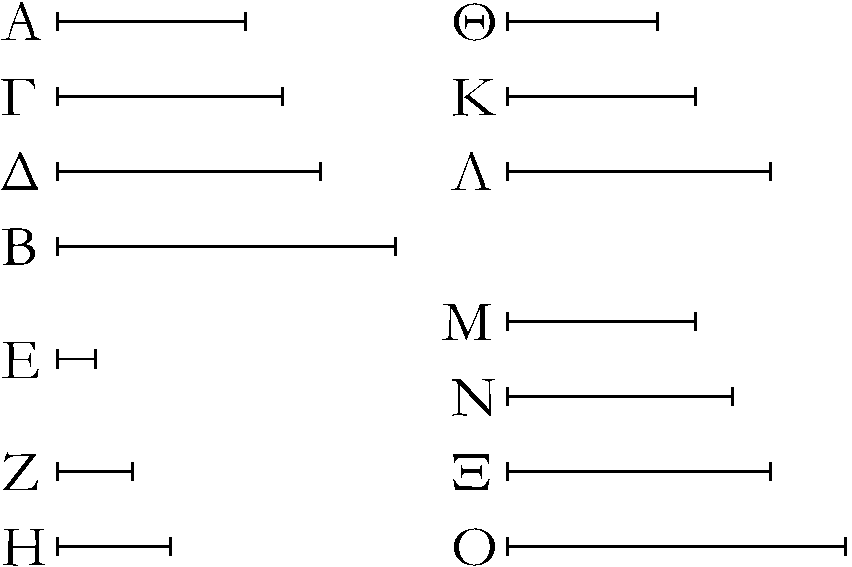
\includegraphics{Book08/fig09g.pdf}}

\gr{>'Εστωσαν δύο ἀριθμοὶ πρῶτοι πρὸξ ἀλλήλουξ οἱ Α, Β, καὶ εἰξ
α\kern -.7pt  ὐτοὺξ μεταχὺ κατὰ τὸ συνεθὲξ ἀνάλογον ἐμπιπτέτωσαν
οἱ Γ, Δ, καὶ ἐκκείσθω ἡ Ε μονάξ; λέγω, <ότι <όσοι εἰξ τοὺξ
Α, Β μεταχὺ κατὰ τὸ συνεθὲξ ἀνάλογον ἐμπεπτώκασιν
ἀριθμοί, τοσοῦτοι καὶ ἑκατέρου τῶν Α, Β καὶ τῆξ μονάδοξ
μεταχὺ κατὰ τὸ συνεθὲξ ἀνάλογον ἐμπεσοῦνται.}

\gr{Εἰλήφθωσαν γὰρ δύο μὲν ἀριθμοὶ ἐλάθιστοι ἐν τῶ| τῶν Α, Γ, Δ, Β
λόγῳ >όντεξ οἱ Ζ, Η, τρεῖξ δὲ οἱ Θ, Κ, Λ, καὶ ἀεὶ ἑχῆξ ἑνὶ
πλείουξ, <έωξ >ὰν >ίσον γένηται τὸ πλῆθοξ α\kern -.7pt  ὐτῶν τῶ|
πλήθει τῶν Α, Γ, Δ, Β. εἰλήφθωσαν, καὶ >έστωσαν οἱ Μ, Ν, Χ, Ο.
φανερὸν δή, <ότι ὁ μὲν Ζ ἑαυτὸν πολλαπλασιάσαξ τὸν Θ πεποίηκεν,
τὸν δὲ Θ πολλαπλασιάσαξ τὸν Μ πεποίηκεν, καὶ ὁ Η
ἑαυτὸν μὲν πολλαπλασιάσαξ τὸν Λ πεποίηκεν, τὸν δὲ Λ πολλαπλασιάσαξ τὸν Ο πεποίηκεν.  καὶ ἐπεὶ οἱ Μ, Ν, Χ, Ο ἐλάθιστοί εἰσι τῶν
τὸν α\kern -.7pt  ὐτὸν λόγον ἐθόντων τοῖξ Ζ, Η, εἰσὶ δὲ καὶ οἱ Α, Γ, Δ, Β
ἐλάθιστοι τῶν τὸν α\kern -.5pt  ὐτὸν λόγον ἐθόντων τοῖξ
Ζ, Η, καί ἐστιν >ίσον τὸ πλῆθοξ τῶν Μ, Ν, Χ, Ο τῶ| πλήθει
τῶν Α, Γ, Δ, Β, <έκαστοξ >άρα τῶν Μ, Ν, Χ, Ο ἑκάστῳ
τῶν Α, Γ, Δ, Β >ίσοξ ἐστίν; >ίσοξ >άρα ἐστὶν ὁ μὲν Μ τῶ|
Α, ὁ δὲ Ο τῶ| Β. καὶ ἐπεὶ ὁ Ζ ἑαυτὸν πολλαπλασιάσαξ τὸν Θ πεποίηκεν, ὁ Ζ >άρα τὸν Θ μετρεῖ κατὰ τὰξ ἐν τῶ| Ζ μονάδαξ. μετρεῖ
δὲ καὶ ἡ Ε μονὰξ τὸν Ζ κατὰ τὰξ ἐν α\kern -.3pt  ὐτῶ| μονάδαξ; ἰσάκιξ
>άρα ἡ Ε μονὰξ τὸν Ζ ἀριθμὸν μετρεῖ καὶ ὁ Ζ τὸν Θ. >έστιν
>άρα ὡξ ἡ Ε μονὰξ πρὸξ τὸν Ζ ἀριθμόν, ο<ύτωξ ὁ Ζ πρὸξ τὸν Θ.
πάλιν, ἐπεὶ ὁ Ζ τὸν Θ πολλαπλασιάσαξ τὸν Μ πεποίηκεν, ὁ Θ >άρα
τὸν Μ μετρεῖ κατὰ τὰξ ἐν τῶ| Ζ μονάδαξ. μετρεῖ δὲ καὶ ἡ Ε
μονὰξ τὸν Ζ ἀριθμὸν κατὰ τὰξ ἐν α\kern -.7pt  ὐτῶ| μονάδαξ; ἰσάκιξ
>άρα ἡ Ε μονὰξ τὸν Ζ ἀριθμὸν μετρεῖ καὶ ὁ Θ τὸν Μ. >έστιν
>άρα ὡξ ἡ Ε μονὰξ πρὸξ τὸν Ζ ἀριθμόν, ο<ύτωξ ὁ Θ πρὸξ τὸν Μ.
ἐδείθθη δὲ καὶ ὡξ ἡ Ε μονὰξ πρὸξ τὸν Ζ ἀριθμόν, ο<ύτωξ
ὁ Ζ πρὸξ τὸν Θ; καὶ ὡξ >άρα ἡ Ε μονὰξ πρὸξ τὸν Ζ ἀριθμόν, ο<ύτωξ ὁ Ζ πρὸξ τὸν Θ καὶ ὁ Θ πρὸξ τὸν Μ. >ίσοξ δὲ ὁ Μ 	τῶ|
Α; >έστιν >άρα ὡξ ἡ Ε μονὰξ πρὸξ τὸν Ζ ἀριθμόν, ο<ύτωξ
ὁ Ζ πρὸξ τὸν Θ καὶ ὁ Θ πρὸξ τὸν
Α. διὰ τὰ α\kern -.7pt  ὐτὰ δὴ
καὶ ὡξ ἡ Ε μονὰξ πρὸξ τὸν Η ἀριθμόν, ο<ύτωξ ὁ Η πρὸξ τὸν Λ
καὶ ὁ Λ πρὸξ τὸν Β. <όσοι >άρα εἰξ τοὺξ Α, Β
μεταχὺ κατὰ τὸ
συνεθὲξ ἀνάλογον ἐμπεπτώκασιν ἀριθμοί, τοσοῦτοι καὶ ἑκατέρου
τῶν Α, Β καὶ μονάδοξ τῆξ Ε μεταχὺ κατὰ τὸ συνεθὲξ ἀνάλογον
ἐμπεπτώκασιν ἀριθμοί; <όπερ >έδει δεῖχαι.}}

\ParallelRText{
\begin{center}
{\large Proposition 9}
\end{center}

If two numbers are prime to one another and there fall  in  between them (some) numbers in continued proportion then,
as many numbers as fall in between them  in continued proportion, so many
(numbers) will also fall between each of them and a unit in continued proportion.

% Removed epsf size command
\centerline{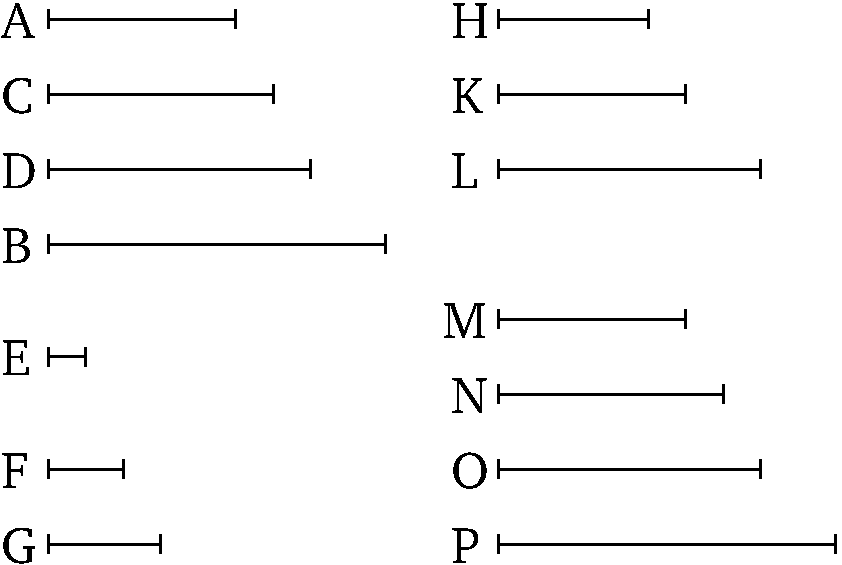
\includegraphics{Book08/fig09e.pdf}}

Let $A$ and $B$ be two numbers (which are) prime to one another, and let the
(numbers) $C$ and $D$ fall in  between them in continued proportion. And let the unit $E$ be set out. I say that, as many numbers   as have fallen in between $A$ and $B$ in continued proportion, so many (numbers)  will also
fall between each of $A$ and $B$ and the unit in continued proportion.

For let the least two numbers, $F$ and $G$, which are in the
ratio of $A$, $C$, $D$, $B$, be taken [Prop.~7.33]. And the (least) three (numbers), $H$, $K$, $L$. And so on, successively increasing by one, until the multitude
of the (least numbers taken) is made  equal to the multitude of $A$, $C$, $D$, $B$
[Prop.~8.2]. Let them be taken, and let
them be $M$, $N$, $O$, $P$. So (it is) clear that $F$ has made $H$ (by)
multiplying itself, and has made $M$ (by) multiplying $H$. And $G$
has made $L$ (by) multiplying itself, and has made $P$ (by) multiplying $L$
[Prop.~8.2~corr.]. And since $M$, $N$, $O$, $P$
are the least of those (numbers) having the same ratio as $F$, $G$, and
$A$, $C$, $D$, $B$ are also the least of those (numbers) having the
same ratio as $F$, $G$ [Prop.~8.2], and the multitude
of $M$, $N$, $O$, $P$ is equal to the multitude of $A$, $C$, $D$, $B$, thus
$M$, $N$, $O$, $P$ are  equal to  $A$, $C$, $D$, $B$, respectively. 
Thus, $M$ is equal to $A$, and $P$ to $B$. And since $F$ has made
$H$ (by) multiplying itself, $F$ thus measures $H$ according to the
units in $F$ [Def.~7.15].  And the unit $E$ also
measures $F$ according to the units in it. Thus, the unit $E$
measures the number $F$ as many times as $F$ (measures) $H$. Thus,
as the unit $E$ is to the number $F$, so $F$ (is) to $H$ [Def.~7.20]. Again, since $F$ has made $M$ (by)
multiplying $H$, $H$ thus measures $M$ according to the units in $F$
 [Def.~7.15].  And the unit $E$ also measures
 the number $F$ according to the units in it. Thus, the unit $E$ measures
 the number $F$ as many times as $H$ (measures) $M$. Thus,
 as the unit $E$ is to the number $F$, so $H$ (is) to $M$ [Prop.~7.20]. And it was shown
 that as the unit $E$ (is) to the number $F$, so $F$ (is) to $H$. And thus
 as the unit $E$ (is) to the number $F$, so $F$ (is) to $H$, and $H$ (is)
 to $M$. And $M$ (is) equal to $A$. Thus, as the unit $E$ is to the number
 $F$, so $F$ (is) to $H$, and $H$ to $A$. And so, for the same (reasons),
 as the unit $E$ (is) to the number $G$, so $G$ (is) to $L$, and $L$ to
 $B$.  Thus, as many  (numbers)  as have fallen
 in between $A$ and $B$  in continued proportion,  so many numbers  have also fallen between each of $A$ and $B$ and the unit 
 $E$ in continued proportion. (Which is) the very thing it was required to show. }
\end{Parallel}

%%%%%%
% Prop 8.10
%%%%%%
\pdfbookmark[1]{Proposition 8.10}{pdf8.10}
\begin{Parallel}{}{} 
\ParallelLText{
\begin{center}
{\large \ggn{10}.}
\end{center}\vspace*{-7pt}

\gr{Ἐάν δύο ἀριθμῶν ἑκατέρου καὶ μονάδοξ μεταχὺ κατὰ τὸ
συνεθὲξ ἀνάλογον ἐμπίπτωσιν ἀριθμοί, <όσοι ἑκατέρου α\kern -.7pt  ὐτῶν
καὶ μονάδοξ μεταχὺ κατὰ τὸ συνεθὲξ ἀνάλογον ἐμπίπτουσιν ἀριθμοί,
τοσοῦτοι καὶ εἰξ α\kern -.7pt  ὐτοὺξ μεταχὺ κατὰ τὸ συνεθὲξ ἀνάλογον
ἐμπεσοῦνται.}

\gr{Δύο γὰρ ἀριθμῶν τῶν Α, Β καὶ μονάδοξ τῆξ Γ μεταχύ κατὰ
τὸ συνεθὲξ ἀνάλογον ἐμπιπτέτωσαν ἀριθμοὶ ο<ί τε Δ, Ε
καὶ οἱ Ζ, Η; λέγω, <ότι <όσοι ἑκατέρου τῶν Α, Β καὶ μονάδοξ
τῆξ Γ μεταχὺ κατὰ τὸ συνεθὲξ ἀνάλογον ἐμπεπτώκασιν
ἀριθμοί, τοσοῦτοι καὶ εἰξ τοὺξ Α, Β μεταχὺ κατὰ τὸ συνεθὲξ
ἀνάλογον ἐμπεσοῦνται.}

% Removed epsf size command
\centerline{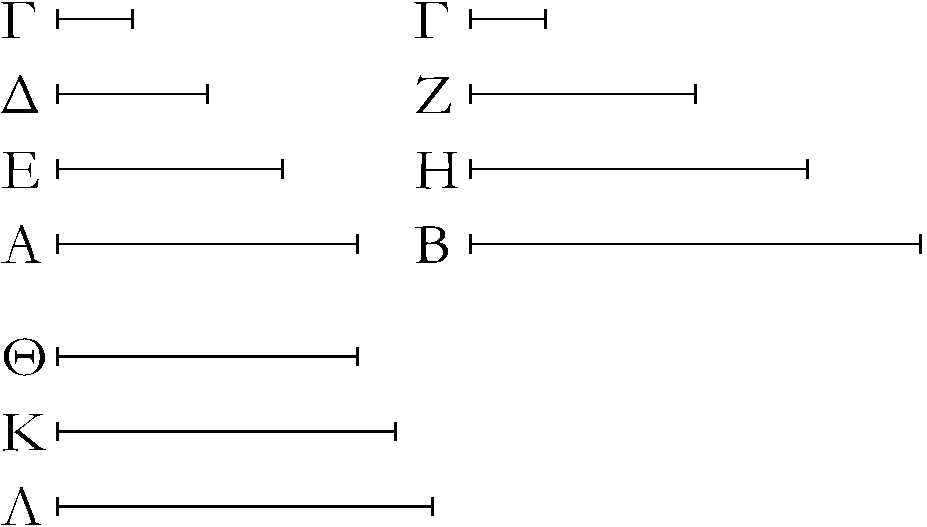
\includegraphics{Book08/fig10g.pdf}}

\gr{Ὁ Δ γὰρ τὸν Ζ πολλαπλασιάσαξ τὸν Θ ποιείτω,
ἑκάτεροξ δὲ τῶν Δ, Ζ τὸν Θ πολλαπλασιάσαξ ἑκάτερον
τῶν Κ, Λ ποιείτω.}

\gr{Καὶ ἐπεί ἐστιν ὡξ ἡ Γ μονὰξ πρὸξ τὸν Δ ἀριθμόν,
ο<ύτωξ ὁ Δ πρὸξ τὸν Ε, ἰσάκιξ >άρα ἡ Γ μονὰξ
τὸν Δ ἀριθμὸν μετρεῖ καὶ ὁ Δ τὸν Ε. ἡ δὲ Γ μονὰξ τὸν
Δ ἀριθμὸν μετρεῖ κατὰ τὰξ ἐν τῶ| Δ μονάδαξ; καὶ ὁ Δ >άρα
ἀριθμὸξ τὸν Ε μετρεῖ κατὰ τὰξ ἐν τῶ| Δ μονάδαξ;  ὁ Δ >άρα
ἑαυτὸν πολλαπλασιάσαξ τὸν Ε πεποίηκεν. πάλιν, ἐπεί
ἐστιν ὡξ ἡ Γ [μονὰξ] πρὸξ τὸν Δ ἀριθμὸν, ο<ύτωξ ὁ Ε πρὸξ
τὸν Α, ἰσάκιξ >άρα ἡ Γ μονὰξ τὸν Δ ἀριθμὸν μετρεῖ καὶ
ὁ Ε τὸν Α. ἡ δὲ Γ μονὰξ τὸν Δ ἀριθμὸν μετρεῖ κατὰ τὰξ ἐν τῶ|
Δ μονάδαξ; καὶ ὁ Ε >άρα τὸν Α μετρεῖ κατὰ τὰξ ἐν τῶ| Δ μονάδαξ; ὁ Δ >άρα τὸν Ε πολλαπλασιάσαξ τὸν Α πεποίηκεν. διὰ
τὰ α\kern -.7pt  ὐτὰ δὴ καὶ ὁ μὲν Ζ ἑαυτὸν πολλαπλασιάσαξ τὸν Η πεποίηκεν,
τὸν δὲ Η πολλαπλασιάσαξ τὸν Β πεποίηκεν. καὶ ἐπεὶ ὁ Δ
ἑαυτὸν μὲν πολλαπλασιάσαξ τὸν Ε πεποίηκεν, τὸν δὲ Ζ πολλαπλασιάσαξ τὸν  Θ πεποίηκεν, >έστιν >άρα ὡξ ὁ Δ πρὸξ τὸν Ζ, ο<ύτωξ ὁ Ε πρὸξ τὸν Θ. διὰ τὰ α\kern -.7pt  ὐτὰ
δὴ καὶ ὡξ ὁ Δ πρὸξ τὸν Ζ, ο<ύτωξ ὁ Θ πρὸξ τὸν Η. καὶ ὡξ
>άρα ὁ Ε πρὸξ τὸν Θ, ο<ύτωξ ὁ Θ πρὸξ τὸν Η. πάλιν, ἐπεὶ
ὁ Δ ἑκάτερον τῶν Ε, Θ πολλαπλασιάσαξ ἑκάτερον τῶν Α, Κ πεποίηκεν,
>έστιν >άρα ὡξ ὁ Ε πρὸξ τὸν Θ, ο<ύτωξ ὁ Α πρὸξ τὸν Κ. ἀλλ>
ὡξ ὁ Ε πρὸξ τὸν Θ, ο<ύτωξ ὁ Δ πρὸξ τὸν Ζ; καὶ ὡξ >άρα ὁ Δ
πρὸξ τὸν Ζ, ο<ύτωξ ὁ Α πρὸξ τὸν Κ. πάλιν, ἐπεὶ ἑκάτεροξ
τῶν Δ, Ζ τὸν Θ πολλαπλασιάσαξ ἑκάτερον τῶν Κ, Λ πεποίηκεν,
<έστιν >άρα ὡξ ὁ Δ πρὸξ τὸν Ζ, ο<ύτωξ ὁ Κ πρὸξ τὸν Λ.
ἀλλ> ὡξ ὁ Δ πρὸξ τὸν Ζ, ο<ύτωξ ὁ Α πρὸξ τὸν Κ;  καὶ ὡξ >άρα
ὁ Α πρὸξ τὸν
 Κ, ο<ύτωξ ὁ
Κ πρὸξ τὸν Λ. >έτι ἐπεὶ ὁ Ζ ἑκάτερον τῶν Θ, Η πολλαπλασιάσαξ
ἑκάτερον τῶν Λ, Β πεποίηκεν,
>έστιν >άρα ὡξ ὁ Θ πρὸξ τὸν Η, ο<ύτωξ ὁ Λ πρὸξ τὸν Β.
ὡξ δὲ ὁ
Θ πρὸξ τὸν Η, ο<ύτωξ ὁ Δ πρὸξ  τὸν Ζ; καὶ ὡξ >άρα ὁ Δ πρὸξ τὸν Ζ,
ο<ύτωξ ὁ Λ πρὸξ τὸν Β. ἐδείθθη δὲ καὶ ὡξ ὁ Δ πρὸξ τὸν Ζ, ο<ύτωξ
<ό τε Α πρὸξ τὸν Κ καὶ ὁ Κ πρὸξ τὸν Λ; καὶ ὡξ >άρα ὁ Α πρὸξ
τὸν Κ, ο<ύτωξ ὁ Κ πρὸξ τὸν Λ καὶ ὁ Λ πρὸξ τὸν Β. οἱ Α, Κ, Λ, Β
>άρα κατὰ τὸ συνεθὲξ ἑχῆξ εἰσιν ἀνάλογον.
<όσοι
>άρα ἑκατέρου τῶν Α, Β καὶ τῆξ Γ μονάδοξ μεταχὺ κατὰ τὸ συνεθὲξ
ἀνάλογον ἐμπίπτουσιν ἀριθμοί, τοσοῦτοι καὶ εἰξ τοὺξ Α, Β
μεταχὺ κατὰ τὸ συνεθὲξ ἐμπεσοῦνται; <όπερ >έδει δεῖχαι.}}

\ParallelRText{
\begin{center}
{\large Proposition 10}
\end{center}

If (some) numbers fall between each of two numbers and a unit in continued proportion then, as many (numbers)
as fall between each of the (two numbers) and the unit in continued proportion, so many (numbers)  will also fall in between the (two numbers) themselves in continued proportion.

For let the numbers $D$, $E$ and $F$, $G$ fall between the numbers $A$ and $B$ (respectively) and the unit $C$ in continued proportion. I say that,
as many numbers as have fallen between each of $A$ and $B$ and the unit $C$ in continued proportion,
so many will also fall in between $A$ and $B$ in continued proportion.\\

% Removed epsf size command
\centerline{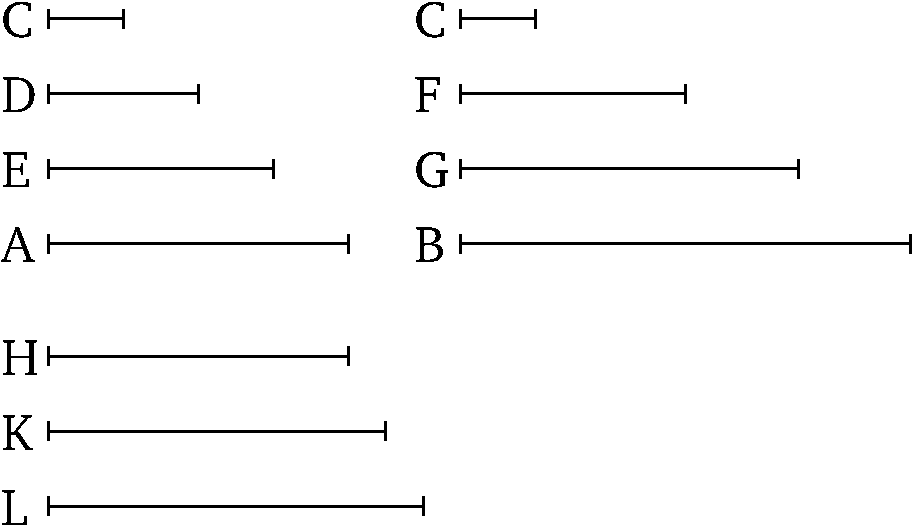
\includegraphics{Book08/fig10e.pdf}}

For let $D$ make $H$ (by) multiplying $F$. And let  $D$, $F$
make $K$, $L$, respectively, by multiplying $H$.

As since as the unit $C$  is to the number $D$, so $D$ (is) to $E$, the unit
$C$ thus measures the number $D$ as many times as $D$ (measures) $E$
[Def.~7.20]. And the unit $C$ measures the
number $D$ according to the units in $D$. Thus, the number $D$
also measures $E$ according to the units in $D$. Thus, $D$ has made $E$
(by) multiplying itself. Again, since as the [unit] $C$ is to
the number $D$, so $E$ (is) to $A$, the unit $C$ thus measures the number
$D$ as many times as $E$ (measures) $A$ [Def.~7.20].
  And the unit $C$ measures the number $D$ according to the units in $D$.
  Thus, $E$ also measures $A$ according to the units  in $D$. Thus, $D$
  has made $A$ (by) multiplying $E$. And so, for the same (reasons), 
  $F$ has made $G$ (by) multiplying itself, and has made $B$ (by)
  multiplying $G$. And since $D$ has made $E$ (by) multiplying itself,
  and has made $H$ (by) multiplying $F$, thus as $D$ is to $F$, so
  $E$ (is) to $H$ [Prop~7.17]. And so, for the
  same reasons, as $D$ (is) to $F$, so $H$ (is) to $G$ [Prop.~7.18].  And thus as $E$ (is) to $H$, so $H$
  (is) to $G$. Again, since $D$ has made  $A$, $K$ (by)
  multiplying $E$, $H$, respectively, thus as $E$ is to $H$, so $A$ (is)
  to $K$ [Prop~7.17]. But, as $E$ (is) to $H$,
  so $D$ (is) to $F$. And thus as $D$ (is) to $F$, so $A$ (is) to $K$.
  Again, since  $D$, $F$ have made  $K$, $L$, respectively, (by) multiplying $H$, thus as $D$ is to $F$, so $K$ (is) to $L$ [Prop.~7.18]. But, as $D$ (is) to $F$, so $A$ (is)
  to $K$.  And thus as $A$ (is) to $K$, so $K$ (is) to $L$.
   Further, since $F$ has made  $L$, $B$ (by) multiplying
   $H$, $G$, respectively, thus as $H$ is to $G$, so $L$ (is) to $B$  [Prop~7.17]. And as $H$ (is) to $G$, so $D$ (is) to $F$. And thus as $D$ 
  (is) to $F$, so $L$ (is) to $B$. And it was also
  shown that as $D$ (is) to $F$, so $A$ (is) to $K$, and $K$ to $L$.
  And thus as $A$ (is) to $K$, so $K$ (is) to $L$, and $L$ to $B$.
  Thus, $A$, $K$, $L$, $B$ are  successively in continued proportion.
  Thus, as many numbers as fall between each of $A$ and $B$ and the unit $C$ in continued proportion, so many will also fall in between $A$ and $B$
  in continued proportion. (Which is) the very thing it was required to show.}
\end{Parallel}

%%%%%%
% Prop 8.11
%%%%%%
\pdfbookmark[1]{Proposition 8.11}{pdf8.11}
\begin{Parallel}{}{} 
\ParallelLText{
\begin{center}
{\large \ggn{11}.}
\end{center}\vspace*{-7pt}

\gr{Δύο τετραγώνων ἀριθμῶν ε<ῖξ μέσοξ ἀνάλογόν ἐστιν ἀριθμόξ,
καὶ ὁ τετράγωνοξ πρὸξ τὸν τετράγωνον διπλασίονα λόγον >έθει
>ήπερ ἡ πλευρὰ πρὸξ τὴν πλευράν.}\\

% Removed epsf size command
\centerline{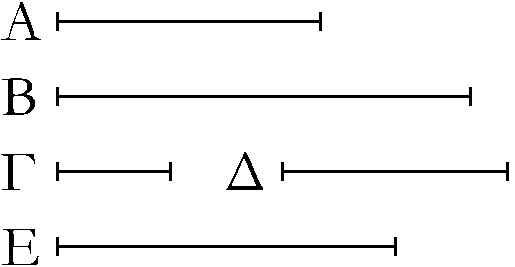
\includegraphics{Book08/fig11g.pdf}}

\gr{>'Εστωσαν τετράγωνοι ἀριθμοὶ οἱ Α, Β, καὶ τοῦ μὲν Α πλευρὰ
>έστω ὁ Γ, τοῦ δὲ Β ὁ Δ; λέγω, <ότι τῶν Α, Β ε<ῖξ
μέσοξ ἀνάλογόν ἐστιν ἀριθμόξ, καὶ ὁ Α πρὸξ τὸν Β
διπλασίονα λόγον >έθει >ήπερ ὁ Γ πρὸξ τὸν Δ.}

\gr{Ὁ Γ γὰρ τὸν Δ πολλαπλασιάσαξ τὸν Ε ποιείτω. καὶ ἐπεὶ τετράγωνόξ
ἐστιν ὁ Α, πλευρὰ δὲ α\kern -.7pt  ὐτοῦ ἐστιν ὁ Γ, ὁ Γ >άρα ἑαυτὸν
πολλαπλασιάσαξ τὸν Α πεποίηκεν. διὰ τὰ α\kern -.7pt  ὐτὰ
δὴ καὶ ὁ Δ ἑαυτὸν πολλαπλασιάσαξ τὸν Β πεποίηκεν.
ἐπεὶ ο>ῦν
ὁ Γ ἑκάτερον τῶν Γ, Δ πολλαπλασιάσαξ ἑκάτερον τῶν Α, Ε πεποίηκεν,
>έστιν >άρα ὡξ ὁ Γ πρὸξ τὸν Δ, ο<ύτωξ ὁ Α πρὸξ τὸν Ε. διὰ
τὰ α\kern -.5pt  ὐτὰ δὴ καὶ ὡξ ὁ Γ πρὸξ τὸν Δ, ο<ύτωξ ὁ Ε πρὸξ τὸν Β.
καὶ ὡξ >άρα ὁ Α πρὸξ τὸν Ε, ο<ύτωξ ὁ Ε πρὸξ τὸν Β. τῶν Α, Β
>άρα ε<ῖξ μέσοξ ἀνάλογόν ἐστιν ἀριθμόξ.}

\gr{Λέγω δή, <ότι καὶ ὁ Α πρὸξ τὸν Β διπλασίονα λόγον >έθει >ήπερ
ὁ Γ πρὸξ τὸν Δ. ἐπεὶ γὰρ τρεῖξ ἀριθμοὶ ἀνάλογόν εἰσιν
οἱ Α, Ε, Β, ὁ Α >άρα πρὸξ τὸν Β διπλασίονα λόγον >έθει
>ήπερ ὁ Α πρὸξ τὸν Ε. ὡξ δὲ ὁ Α πρὸξ τὸν Ε, ο<ύτωξ ὁ Γ
πρὸξ τὸν Δ. ὁ Α >άρα πρὸξ τὸν Β διπλασίονα λόγον >έθει
>ήπερ ἡ Γ πλευρὰ πρὸξ τὴν Δ; <όπερ >έδει δεῖχαι.}}

\ParallelRText{
\begin{center}
{\large Proposition 11}
\end{center}

There exists one number in mean proportion to two (given) square numbers.$^\dag$ And (one)  square (number) has to the
(other) square (number) a squared$^\ddag$ ratio with respect to (that) the side (of the former
has) to the side (of the latter).

% Removed epsf size command
\centerline{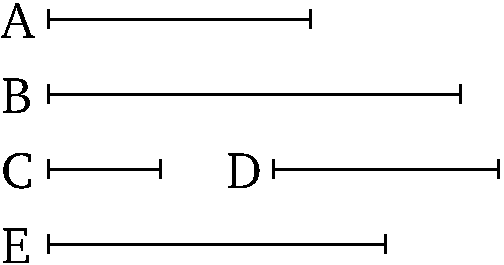
\includegraphics{Book08/fig11e.pdf}}

Let $A$ and $B$ be square numbers, and let $C$ be the side of $A$, and
$D$ (the side) of $B$. I say that there exists one number in mean proportion
to $A$ and $B$, and that $A$ has to $B$ a squared ratio with respect to
(that) $C$ (has) to $D$.

For let $C$ make $E$ (by) multiplying $D$. And since $A$ is square, and $C$ is its side, $C$ has thus made $A$ (by) multiplying
itself. And so, for the same (reasons), $D$ has made $B$ (by) multiplying
itself. Therefore, since $C$ has made  $A$, $E$ (by) multiplying
$C$, $D$, respectively, thus as $C$ is to $D$, so $A$ (is) to $E$ [Prop.~7.17]. And so, for the same (reasons), 
as $C$ (is) to $D$, so $E$ (is) to $B$  [Prop.~7.18]. And thus as $A$ (is) to $E$, so
$E$ (is) to $B$. Thus,  one  number (namely, $E$) is in mean proportion to $A$ and $B$.

So I say that $A$ also has to $B$ a squared ratio with respect to (that)
$C$ (has) to $D$. For since $A$, $E$, $B$ are  three (continuously) proportional numbers, $A$ thus has to $B$ a squared ratio with
respect to (that) $A$ (has) to $E$ [Def.~5.9]. And
as $A$ (is) to $E$, so $C$ (is) to $D$. Thus, $A$ has to $B$ a squared ratio
with respect to (that) side $C$ (has) to (side) $D$. (Which is) the very thing it
was required to show.}
\end{Parallel}
{\footnotesize\noindent$^\dag$ In other words, between two given square numbers there
exists a number in continued proportion.\\[0.5ex]
$^\ddag$ Literally, ``double''.}

%%%%%%
% Prop 8.12
%%%%%%
\pdfbookmark[1]{Proposition 8.12}{pdf8.12}
\begin{Parallel}{}{} 
\ParallelLText{
\begin{center}
{\large \ggn{12}.}
\end{center}\vspace*{-7pt}

\gr{Δύο κύβων ἀριθμῶν δύο μέσοι ἀνάλογόν εἰσιν ἀριθμοί, καὶ
ὁ κύβοξ πρὸξ τὸν κύβον τριπλασίονα λόγον >έθει >ήπερ ἡ πλευρὰ πρὸξ τὴν πλευράν.}

\gr{>'Εστωσαν κύβοι ἀριθμοὶ οἱ Α, Β καὶ τοῦ μὲν Α πλευρὰ >έστω
ὁ Γ, τοῦ δὲ Β ὁ Δ; λέγω, <ότι τῶν Α, Β δύο μέσοι ἀνάλογόν
εἰσιν ἀριθμοί, καὶ ὁ Α πρὸξ τὸν Β τριπλασίονα λόγον >έθει
>ήπερ ὁ Γ πρὸξ τὸν Δ. }\\

% Removed epsf size command
\centerline{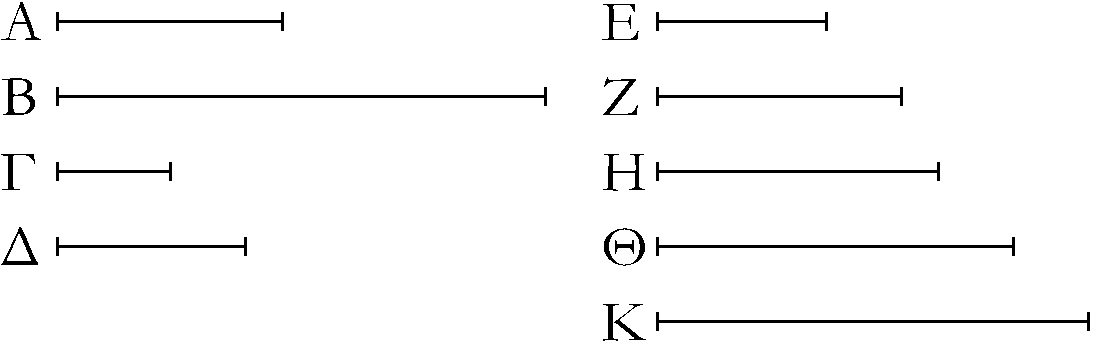
\includegraphics{Book08/fig12g.pdf}}

\gr{Ὁ γὰρ Γ ἑαυτὸν μὲν πολλαπλασιάσαξ τὸν Ε ποιείτω, τὸν δὲ Δ πολλαπλασιάσαξ τὸν Ζ ποιείτω, ὁ δὲ Δ ἑαυτὸν πολλαπλασιάσαξ τὸν Η ποιείτω, ἑκάτεροξ δὲ τῶν Γ, Δ τὸν Ζ πολλαπλασιάσαξ ἑκάτερον
τῶν Θ, Κ ποιείτω.}

\gr{Καὶ ἐπεὶ κύβοξ ἐστὶν ὁ Α, πλευρὰ δὲ α\kern -.7pt  ὐτοῦ ὁ Γ, καὶ ὁ Γ
ἑαυτὸν μὲν πολλαπλασιάσαξ τὸν Ε πεποίηκεν, ὁ Γ >άρα ἑαυτὸν
μὲν πολλαπλασιάσαξ τὸν Ε πεποίηκεν, τὸν δὲ Ε πολλαπλασιάσαξ τὸν Α
πεποίηκεν. διὰ τὰ α\kern -.7pt  ὐτὰ δὴ καὶ ὁ Δ ἑαυτὸν μὲν πολλαπλασιάσαξ
τὸν Η πεποίηκεν, τὸν δὲ Η πολλαπλασιάσαξ τὸν Β πεποίηκεν. καὶ
ἐπεὶ ὁ Γ ἑκάτερον τῶν Γ, Δ πολλαπλασιάσαξ ἑκάτερον τῶν Ε, Ζ
πεποίηκεν, >έστιν >άρα ὡξ ὁ Γ πρὸξ τὸν Δ, ο<ύτωξ ὁ Ε πρὸξ
τὸν Ζ. διὰ τὰ α\kern -.5pt  ὐτὰ δὴ καὶ ὡξ ὁ Γ πρὸξ τὸν Δ, ο<ύτωξ 
ὁ Ζ πρὸξ τὸν Η. πάλιν, ἐπεὶ ὁ Γ ἑκάτερον τῶν Ε, Ζ πολλαπλασιάσαξ
ἑκάτερον τῶν Α, Θ πεποίηκεν, >έστιν >άρα ὡξ ὁ Ε πρὸξ τὸν Ζ, ο<ύτωξ
ὁ Α πρὸξ τὸν Θ. ὡξ δὲ ὁ Ε πρὸξ τὸν Ζ, ο<ύτωξ ὁ Γ πρὸξ τὸν Δ;
καὶ ὡξ >άρα ὁ Γ πρὸξ τὸν Δ, ο<ύτωξ ὁ Α πρὸξ τὸν Θ. πάλιν,
ἐπεὶ ἑκάτεροξ τῶν Γ, Δ τὸν Ζ πολλαπλασιάσαξ ἑκάτερον τῶν
Θ, Κ πεποίηκεν, >έστιν >άρα ὡξ ὁ Γ πρὸξ τὸν Δ, ο<ύτωξ ὁ Θ
πρὸξ τὸν Κ. πάλιν, ἐπεὶ ὁ Δ ἑκάτερον τῶν Ζ, Η πολλαπλασιάσαξ
ἑκάτερον τῶν Κ, Β πεποίηκεν, >έστιν >άρα ὡξ ὁ Ζ πρὸξ τὸν Η,
ο<ύτωξ ὁ Κ πρὸξ τὸν Β. ὡξ δὲ ὁ Ζ πρὸξ τὸν Η, ο<ύτωξ
ὁ Γ πρὸξ τὸν Δ; καὶ ὡξ >άρα ὁ Γ πρὸξ τὸν Δ, ο<ύτωξ
<ό τε Α πρὸξ τὸν Θ καὶ ὁ Θ πρὸξ τὸν Κ καὶ ὁ Κ πρὸξ τὸν Β. τῶν Α, Β >άρα
δύο μέσοι ἀνάλογόν εἰσιν οἱ Θ, Κ.}

\gr{Λέγω δή, <ότι καὶ ὁ Α πρὸξ τὸν Β τριπλασίονα λόγον >έθει
>ήπερ ὁ Γ πρὸξ τὸν Δ. ἐπεὶ γὰρ τέσσαρεξ ἀριθμοὶ
ἀνάλογόν εἰσιν οἱ Α, Θ, Κ, Β, ὁ Α >άρα πρὸξ τὸν Β
τριπλασίονα λόγον >έθει >ήπερ ὁ Α πρὸξ τὸν Θ. ὡξ δὲ ὁ Α
πρὸξ τὸν Θ, ο<ύτωξ ὁ Γ πρὸξ τὸν Δ; καὶ ὁ Α [>άρα] πρὸξ
τὸν Β τριπλασίονα λόγον >έθει >ήπερ ὁ Γ πρὸξ τὸν Δ; <όπερ
>έδει δεῖχαι.}}

\ParallelRText{
\begin{center}
{\large Proposition 12}
\end{center}

There exist two numbers in mean proportion to two (given) cube numbers.$^\dag$ And  (one) cube (number)
has to the (other) cube (number) a cubed$^\ddag$ ratio
with respect to (that) the side (of the former has) to the side (of the latter).

Let $A$ and $B$ be cube numbers, and let $C$ be the side of $A$, and
$D$ (the side) of $B$. I say that there exist two numbers in mean proportion
to $A$ and $B$, and that $A$ has to $B$ a cubed ratio with respect to (that)
$C$ (has) to $D$.

% Removed epsf size command
\centerline{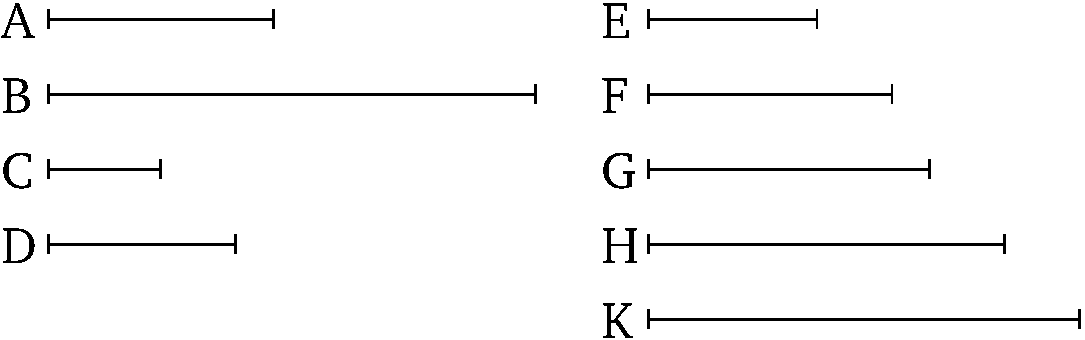
\includegraphics{Book08/fig12e.pdf}}

For let $C$ make $E$ (by) multiplying itself, and let it make
$F$ (by) multiplying $D$. And let $D$ make $G$ (by) multiplying itself,
and let  $C$, $D$ make  $H$, $K$, respectively, (by) multiplying $F$.

And since $A$ is  cube, and $C$ (is) its side, and $C$ has
made $E$ (by) multiplying itself,  $C$ has thus made $E$ (by) multiplying
itself, and has made $A$ (by) multiplying $E$. And so, for the same (reasons),
$D$ has made $G$ (by) multiplying itself, and has made $B$ (by) multiplying $G$. And since $C$ has made  $E$, $F$ (by)
multiplying $C$, $D$, respectively, thus as $C$ is to $D$, so $E$ (is) to $F$
[Prop.~7.17]. And so, for the same (reasons), 
as $C$ (is) to $D$, so $F$ (is) to $G$ [Prop.~7.18].
Again, since $C$ has made  $A$, $H$ (by) multiplying
 $E$, $F$, respectively, thus as $E$ is to $F$, so $A$ (is) to $H$ [Prop.~7.17].  And as $E$ (is) to $F$, so $C$ (is)
to $D$. And thus as $C$ (is) to $D$, so $A$ (is) to $H$. Again,
since  $C$, $D$ have made  $H$, $K$, respectively,  (by) multiplying
$F$, thus as $C$ is to $D$, so $H$ (is) to $K$  [Prop.~7.18].  Again, since $D$ has made $K$, $B$ (by) multiplying  $F$, $G$, respectively, thus as $F$ is to $G$, so $K$ (is) to $B$ [Prop.~7.17]. And as $F$
(is) to $G$, so $C$ (is) to $D$. And thus as $C$ (is) to $D$, so $A$
(is) to $H$, and $H$ to $K$, and $K$ to $B$. Thus, $H$ and $K$ are two
(numbers) in mean proportion to $A$ and $B$.

So I say that $A$ also has to $B$ a cubed ratio with respect to (that)
$C$ (has) to $D$. For since  $A$, $H$, $K$, $B$ are  four 
(continuously) proportional numbers, $A$ thus has to $B$ a cubed ratio with respect to (that)
$A$ (has) to $H$ [Def.~5.10]. And as $A$ (is) to $H$,
so $C$ (is) to $D$. And [thus] $A$ has to $B$ a cubed ratio
with respect to (that) $C$ (has) to $D$. (Which is) the very thing it was required to show.}
\end{Parallel}
{\footnotesize\noindent$^\dag$ In other words, between two given cube numbers there
exist two numbers in continued proportion.\\[0.5ex]
$^\ddag$ Literally, ``triple".}

%%%%%%
% Prop 8.13
%%%%%%
\pdfbookmark[1]{Proposition 8.13}{pdf8.13}
\begin{Parallel}{}{} 
\ParallelLText{
\begin{center}
{\large \ggn{13}.}
\end{center}\vspace*{-7pt}

\gr{Ἐὰν >ῶσιν ὁσοιδηποτοῦν ἀριθμοὶ ἑχῆξ ἀνάλογον, καὶ
πολλαπλασιάσαξ <έκαστοξ ἑαυτὸν ποιῆ| τινα, οἱ γενόμενοι ἐχ
α\kern -.7pt  ὐτῶν ἀνάλογον >έσονται; καὶ ἒαν οἱ ἐχ ἀρθῆξ τοὺξ
γενομένουξ πολλαπλασιάσαντεξ ποιῶσί τιναξ, καὶ α\kern -.7pt  ὐτοὶ ἀνάλογον
>έσονται [καὶ ἀεὶ περὶ τοὺξ >άκρουξ τοῦτο συμβαίνει].}

\gr{>'Εστωσαν ὁποσοιοῦν ἀριθμοὶ ἑχῆξ ἀνάλογον, οἱ Α, Β, Γ,
ὡξ ὁ Α πρὸξ τὸν Β, ο<ύτωξ ὁ Β πρὸξ τὸν Γ, καὶ οἱ Α, Β, Γ
ἑαυτοὺξ μὲν πολλαπλασιάσαντεξ τοὺξ Δ, Ε, Ζ ποιείτωσαν, τοὺξ δὲ
Δ, Ε, Ζ πολλαπλασιάσαντεξ τοὺξ Η, Θ, Κ ποιείτωσαν; λέγω, <ότι
ο<ί τε Δ, Ε, Ζ καὶ οἱ Η, Θ, Κ ἑχῆξ ἀνάλογον εἰσιν.}\\~\\

% Removed epsf size command
\centerline{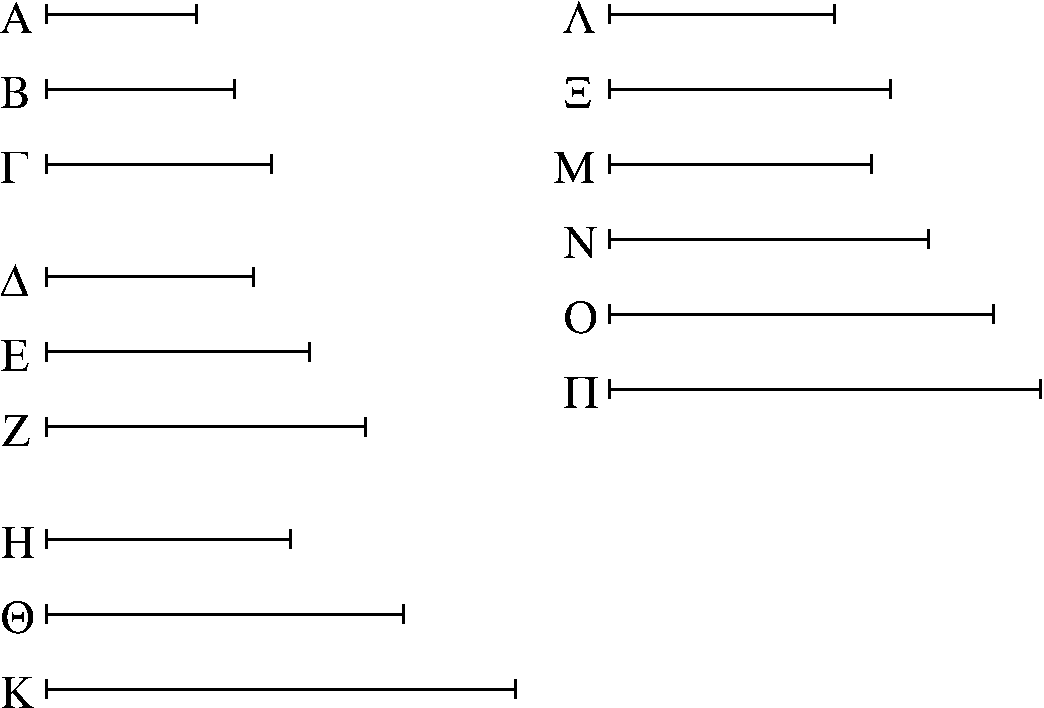
\includegraphics{Book08/fig13g.pdf}}

\gr{Ὁ μὲν γὰρ Α τὸν Β πολλαπλασιάσαξ τὸν Λ ποιείτω, ἑκάτεροξ δὲ
τῶν Α, Β τὸν Λ πολλαπλασιάσαξ ἑκάτερον τῶν Μ, Ν ποιείτω. καὶ
πάλιν ὁ μὲν Β τὸν Γ πολλαπλασιάσαξ τὸν Χ ποιείτω, ἑκάτεροξ
δὲ τῶν Β, Γ τὸν Χ πολλαπλασιάσαξ ἑκάτερον τῶν Ο, Π
ποιείτω.}

\gr{Ὁμοίωξ δὴ τοῖξ ἐπάνω δεῖχομεν, <ότι οἱ Δ, Λ, Ε
καὶ οἱ Η, Μ, Ν, Θ ἑχῆξ εἰσιν ἀνάλογον ἐν τῶ| τοῦ Α πρὸξ
τὸν Β λόγῳ, καὶ >έτι οἱ Ε, Χ, Ζ καὶ οἱ Θ, Ο, Π, Κ ἑχῆξ
εἰσιν ἀνάλογον ἐν τῶ| τοῦ Β πρὸξ τὸν Γ λόγῳ. καί ἐστιν ὡξ ὁ Α
πρὸξ τὸν Β, ο<ύτωξ ὁ Β πρὸξ τὸν Γ; καὶ οἱ Δ, Λ, Ε >άρα τοῖξ Ε, Χ, Ζ
ἐν τῶ| α\kern -.7pt  ὐτῶ| λόγῳ εἰσὶ καὶ >έτι οἱ Η, Μ, Ν, Θ τοῖξ Θ, Ο, Π,
Κ. καί ἐστιν >ίσον τὸ μὲν τῶν Δ, Λ, Ε πλῆθοξ τῶ| τῶν Ε, Χ, Ζ
πλήθει, τὸ δὲ τῶν Η, Μ, Ν, Θ τῶ| τῶν Θ, Ο, Π, Κ;
δι> >ίσου >άρα ἐστὶν ὡξ μὲν ὁ Δ πρὸξ τὸν Ε, ο<ύτωξ ὁ Ε πρὸξ
τὸν Ζ, ὡξ δὲ ὁ Η πρὸξ τὸν Θ, ο<ύτωξ ὁ Θ πρὸξ τὸν Κ; <όπερ
>έδει δεῖχαι.}}

\ParallelRText{
\begin{center}
{\large Proposition 13}
\end{center}

If there are any multitude whatsoever of continuously proportional numbers, and each makes some (number by) multiplying itself, then the (numbers) created from them will
(also) be (continuously) proportional. And if the original (numbers) make some
(more numbers by) multiplying the created (numbers) then these will also be (continuously) proportional [and this always happens with the extremes].

Let $A$, $B$, $C$ be any multitude whatsoever of continuously proportional numbers, (such that) as $A$ (is) to $B$, so $B$ (is) to $C$. And
let $A$, $B$, $C$ make $D$, $E$, $F$ (by) multiplying themselves,
and let them make $G$, $H$, $K$ (by) multiplying $D$, $E$, $F$. 
I say that $D$, $E$, $F$ and $G$, $H$, $K$ are continuously proportional.

% Removed epsf size command
\centerline{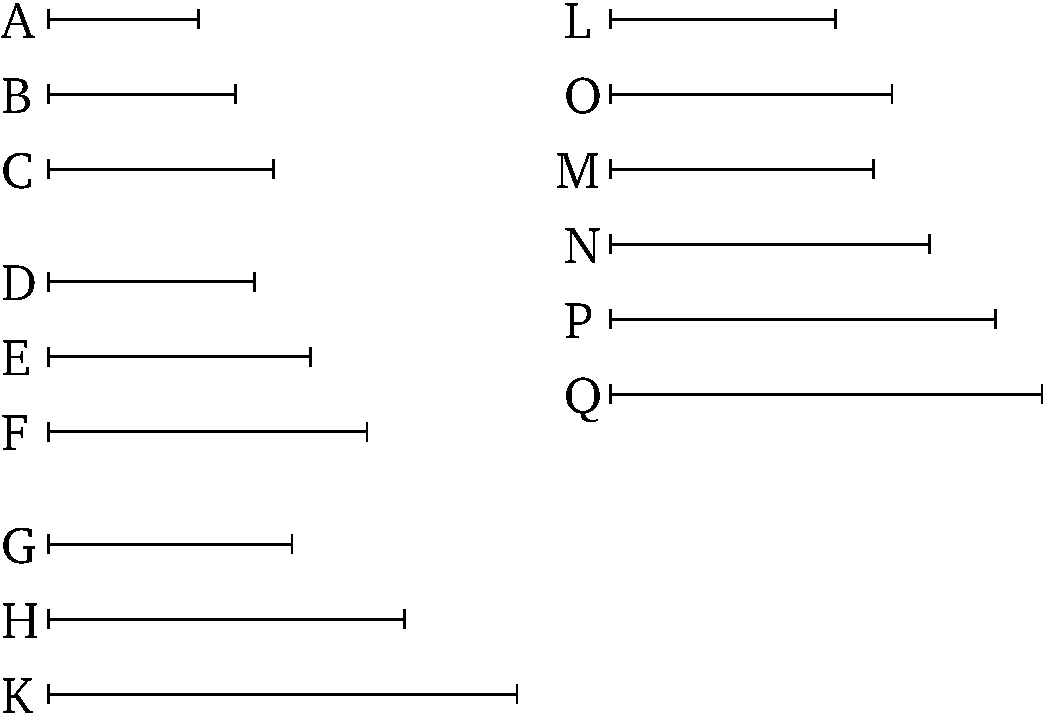
\includegraphics{Book08/fig13e.pdf}}

For let $A$ make $L$ (by) multiplying $B$. And let  $A$, $B$
make  $M$, $N$, respectively, (by) multiplying $L$. And, again, let
$B$ make $O$ (by) multiplying $C$. And let  $B$, $C$
make  $P$, $Q$, respectively, (by) multplying $O$.

So, similarly to the above, we can show that $D$, $L$, $E$ and
$G$, $M$, $N$, $H$ are continuously proportional in the ratio of
$A$ to $B$, and, further, (that) $E$, $O$, $F$ and $H$, $P$, $Q$, $K$
are continuously proportional in the ratio of $B$ to $C$. And as $A$ is to $B$, so $B$ (is) to $C$. And thus $D$, $L$, $E$ are in the same ratio as
$E$, $O$, $F$, and, further, $G$, $M$, $N$, $H$ (are in the same ratio)
as $H$, $P$, $Q$, $K$. And the multitude of $D$, $L$, $E$ is equal
to the multitude of $E$, $O$, $F$, and that of $G$, $M$, $N$, $H$ to that of $H$, $P$, $Q$, $K$. Thus, via equality, as $D$ is to $E$, so $E$ (is) to $F$, and
as $G$ (is) to $H$, so $H$ (is) to $K$ [Prop.~7.14]. (Which is) the very thing it was required to show.}
\end{Parallel}

%%%%%%
% Prop 8.14
%%%%%%
\pdfbookmark[1]{Proposition 8.14}{pdf8.14}
\begin{Parallel}{}{} 
\ParallelLText{
\begin{center}
{\large \ggn{14}.}
\end{center}\vspace*{-7pt}

\gr{Ἐὰν τετράγωνοξ τετράγωνον μετρῆ|, καὶ ἡ πλευρὰ τὴν πλευρὰν
μετρήσει; καὶ ἒαν
ἡ πλευρὰ τὴν πλευρὰν μετρῆ|, καὶ ὁ τετράγωνοξ τὸν τετράγωνον
μετρήσει.}

\gr{>'Εστωσαν τετράγωνοι ἀριθμοὶ οἱ Α, Β, πλευραὶ δὲ α\kern -.7pt  ὐτῶν >έστωσαν
οἱ Γ, Δ, ὁ δὲ Α τὸν Β μετρείτω; λέγω, <ότι καὶ ὁ Γ
τὸν Δ μετρεῖ.}\\~\\

% Removed epsf size command
\centerline{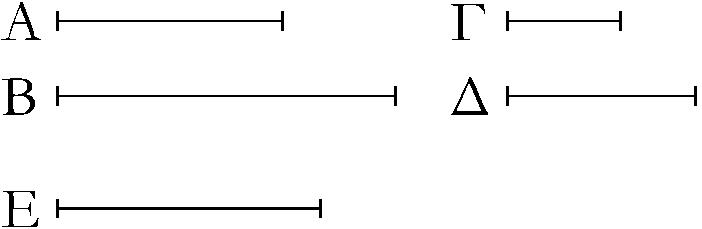
\includegraphics{Book08/fig14g.pdf}}

\gr{Ὁ Γ γὰρ τὸν Δ πολλαπλασιάσαξ τὸν Ε ποιείτω;
οἱ Α, Ε, Β >άρα ἑχῆξ ἀνάλογόν εἰσιν ἐν τῶ| τοῦ Γ πρὸξ
τὸν Δ λόγῳ. καὶ ἐπεὶ οἱ Α, Ε, Β ἐχῆξ ἀνάλογόν εἰσιν, καὶ
μετρεῖ ὁ Α τὸν Β, μετρεῖ >άρα καὶ ὁ Α τὸν Ε. καί ἐστιν ὡξ ὁ
Α πρὸξ τὸν Ε, ο<ύτωξ ὁ Γ πρὸξ τὸν Δ; μετρεῖ >άρα καὶ ὁ Γ
τὸν Δ.}

\gr{Πάλιν δὴ ὁ Γ τὸν Δ μετρείτω; λέγω, <ότι καὶ ὁ Α τὸν Β μετρεῖ.}

\gr{Τῶν γὰρ α\kern -.7pt  ὐτῶν κατασκευασθέντων ὁμοίωξ δείχομεν, <ότι
οἱ Α, Ε, Β ἑχῆξ ἀνάλογόν εἰσιν ἐν τῶ| τοῦ Γ πρὸξ τὸν Δ
λόγῳ. καὶ ἐπεί ἐστιν ὡξ ὁ Γ πρὸξ τὸν Δ, ο<ύτωξ ὁ Α πρὸξ
τὸν Ε, μετρεῖ δὲ ὁ Γ τὸν Δ, μετρεῖ >άρα καὶ ὁ Α τὸν Ε. καί
εἰσιν οἱ Α, Ε, Β ἑχῆξ ἀνάλογον; μετρεῖ >άρα καὶ ὁ Α τὸν Β.}

\gr{Ἐὰν >άρα τετράγωνοξ τετράγωνον μετρῆ|, καὶ ἡ πλευρὰ τὴν πλευρὰν
μετρήσει; καὶ ἒαν ἡ πλευρὰ τὴν πλευρὰν μετρῆ|, καὶ ὁ
τετράγωνοξ τὸν τετράγωνον μετρήσει; <όπερ >έδει δεῖχαι.}}

\ParallelRText{
\begin{center}
{\large Proposition 14}
\end{center}

If a square (number) measures a(nother) square
(number) then the side (of the former) will also measure the
side (of the latter). And if the side (of a square number) measures the side
(of another square number) then the (former) square (number) will also
measure the (latter) square (number).

Let $A$ and $B$ be square numbers, and let $C$ and $D$ be their sides (respectively). And let $A$ measure $B$. I say that $C$ also measures $D$.

% Removed epsf size command
\centerline{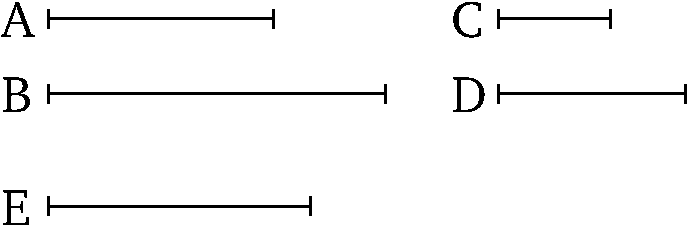
\includegraphics{Book08/fig14e.pdf}}

For let $C$ make $E$ (by) multiplying $D$. Thus, $A$, $E$, $B$
are continuously proportional in the ratio of $C$ to $D$
[Prop.~8.11]. And since $A$, $E$, $B$ are
continuously proportional, and $A$ measures $B$, $A$ thus also
measures $E$ [Prop.~8.7]. And as $A$ is to $E$,
so $C$ (is) to $D$. Thus, $C$ also measures $D$ [Def.~7.20].

So, again, let $C$ measure $D$. I say that $A$ also measures $B$.

For similarly, with the same construction, we can show that $A$, $E$, $B$
are continuously proportional in the ratio of $C$ to $D$. And since as $C$
is to $D$, so $A$ (is) to $E$, and $C$ measures $D$, $A$ thus
also measures $E$ [Def.~7.20]. And $A$, $E$,
$B$ are continuously proportional. Thus, $A$ also measures $B$.

Thus, if a square (number) measures a(nother) square
(number) then the side (of the former) will also measure the
side (of the latter). And if the side (of a square number) measures the side
(of another square number) then the (former) square (number) will also
measure the (latter) square (number). (Which is) the very thing it was
required to show.}
\end{Parallel}

%%%%%%
% Prop 8.15
%%%%%%
\pdfbookmark[1]{Proposition 8.15}{pdf8.15}
\begin{Parallel}{}{} 
\ParallelLText{
\begin{center}
{\large \ggn{15}.}
\end{center}\vspace*{-7pt}

\gr{Ἐὰν κύβοξ ἀριθμὸξ κύβον ἀριθμὸν μετρῆ|, καὶ ἡ πλευρὰ τὴν
πλευρὰν μετρήσει; καὶ ἒαν ἡ πλευρὰ τὴν πλευρὰν μετρῆ|, καὶ
ὁ κύβοξ τὸν κύβον μετρήσει.}

\gr{Κύβοξ γὰρ ἀριθμὸξ ὁ Α κύβον τὸν Β μετρείτω, καὶ τοῦ μὲν
Α πλευρὰ >έστω ὁ Γ, τοῦ δὲ Β ὁ Δ; λέγω, <ότι ὁ Γ τὸν Δ μετρεῖ.}

\gr{Ὁ Γ γὰρ ἑαυτὸν πολλαπλασιάσαξ τὸν Ε ποιείτω, ὁ δὲ Δ ἑαυτὸν
πολλαπλασιάσαξ τὸν Η ποιείτω, καὶ >έτι ὁ Γ τὸν Δ πολλαπλασιάσαξ τὸν Ζ
[ποιείτω], ἑκάτεροξ δὲ τῶν Γ, Δ τὸν Ζ πολλαπλασιάσαξ ἑκάτερον
τῶν Θ, Κ ποιείτω. φανερὸν δή, <ότι οἱ Ε, Ζ, Η καὶ οἱ Α, Θ, Κ, Β
ἑχῆξ ἀνάλογόν εἰσιν ἐν τῶ| τοῦ Γ πρὸξ τὸν Δ λόγῳ. καὶ ἐπεὶ οἱ Α, Θ, Κ, Β ἑχῆξ ἀνάλογόν εἰσιν, καὶ μετρεῖ ὁ Α τὸν Β, μετρεῖ
>άρα καὶ τὸν Θ. καί ἐστιν ὡξ ὁ Α πρὸξ τὸν Θ, ο<ύτωξ ὁ Γ πρὸξ τὸν
Δ; μετρεῖ >άρα καὶ ὁ Γ τὸν Δ.}\\~\\

% Removed epsf size command
\centerline{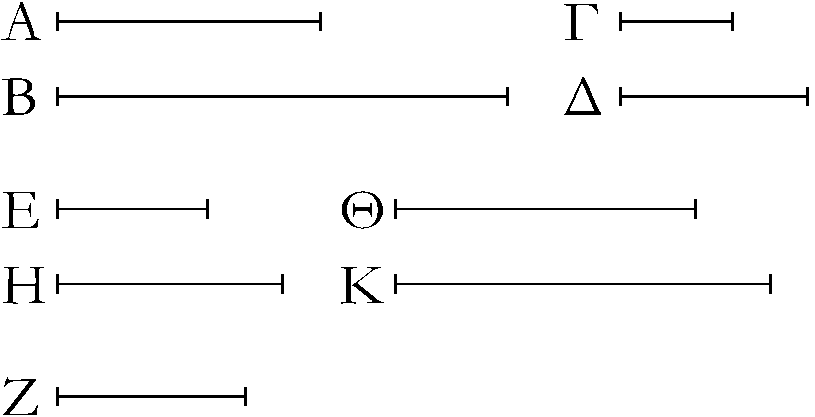
\includegraphics{Book08/fig15g.pdf}}

\gr{Ἀλλὰ δὴ μετρείτω ὁ Γ τὸν Δ; λέγω, <ότι καὶ ὁ Α τὸν Β μετρήσει.}

\gr{Τῶν γὰρ α\kern -.7pt  ὐτῶν κατασκευασθέντων ὁμοίωξ δὴ δείχομεν, <ότι
οἱ Α, Θ, Κ, Β ἑχῆξ ἀνάλογόν εἰσιν ἐν τῶ| τοῦ Γ πρὸξ
τὸν Δ λόγῳ. καὶ ἐπεὶ ὁ Γ τὸν Δ μετρεῖ, καί ἐστιν ὡξ ὁ Γ πρὸξ
τὸν Δ, ο<ύτωξ ὁ Α πρὸξ τὸν Θ, καὶ ὁ Α >άρα τὸν Θ μετρεῖ; <ώστε
καὶ τὸν Β μετρεῖ ὁ Α; <όπερ >έδει δεῖχαι.}}

\ParallelRText{
\begin{center}
{\large Proposition 15}
\end{center}

If a cube number measures a(nother) cube
number then the side (of the former) will also measure the side (of the latter).
And if the side (of a cube number) measures the side (of another cube
number) then the (former) cube (number) will also measure the (latter)
cube (number).

For let the cube number $A$ measure the cube (number) $B$, and let
$C$ be the side of $A$, and $D$ (the side) of $B$. I say that $C$ measures $D$.

For let $C$ make $E$ (by) multiplying itself. And let $D$ make $G$ (by)
multiplying itself. And, further, [let] $C$ [make] $F$ (by) multiplying
$D$,  and let  $C$, $D$ make  $H$, $K$, respectively, (by) multiplying
$F$. So it is clear that $E$, $F$, $G$ and $A$, $H$, $K$, $B$ are continuously proportional in the ratio of $C$ to $D$ [Prop.~8.12]. And since $A$, $H$, $K$, $B$ are
continuously proportional, and $A$ measures $B$, ($A$) thus also
measures $H$ [Prop.~8.7]. And as $A$ is to
$H$, so $C$ (is) to $D$. Thus, $C$ also measures $D$ [Def.~7.20].\\

% Removed epsf size command
\centerline{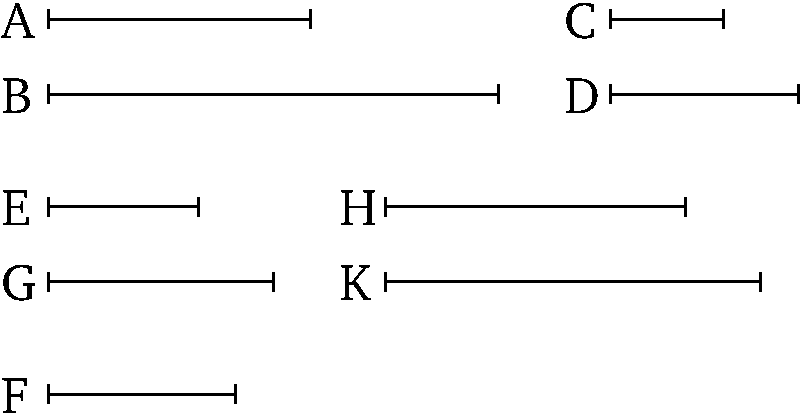
\includegraphics{Book08/fig15e.pdf}}

And so let $C$ measure $D$. I say that $A$ will also measure $B$.

For similarly, with the same construction, we can show that $A$, $H$, $K$, $B$ are continuously proportional in the ratio of $C$ to $D$. And since
$C$ measures $D$, and as $C$ is to $D$, so $A$ (is) to $H$, $A$ thus
also measures $H$ [Def.~7.20]. Hence, $A$ also measures $B$. (Which is) the
very thing it was required to show.}
\end{Parallel}

%%%%%%
% Prop 8.16
%%%%%%
\pdfbookmark[1]{Proposition 8.16}{pdf8.16}
\begin{Parallel}{}{} 
\ParallelLText{
\begin{center}
{\large \ggn{16}.}
\end{center}\vspace*{-7pt}

\gr{Ἐὰν τετράγωνοξ ἀριθμὸξ τετράγωνον ἀριθμὸν μ\kern -.7pt  ὴ μετρῆ|, οὐδὲ
ἡ πλευρὰ τὴν πλευρὰν μετρήσει; κ>ὰν ἡ πλευρὰ τὴν πλευρὰν  μ\kern -.7pt  ὴ
μετρῆ|, οὐδὲ ὁ τετράγωνοξ τὸν τετράγωνον μετρήσει.}\\~\\

% Removed epsf size command
\centerline{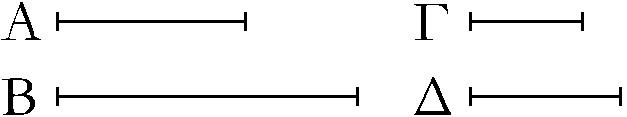
\includegraphics{Book08/fig16g.pdf}}

\gr{>'Εστωσαν τετρὰγωνοι ἀριθμοὶ οἱ Α, Β, πλευραὶ δὲ α\kern -.7pt  ὐτῶν >έστωσαν
οἱ Γ, Δ, καὶ μ\kern -.7pt  ὴ μετρείτω ὁ Α τὸν Β; λὲγω, <ότι οὐδὲ ὁ Γ τὸν Δ
μετρεῖ.}

\gr{Εἰ γὰρ μετρεῖ ὁ Γ τὸν Δ, μετρήσει καὶ ὁ Α τὸν Β. οὐ μετρεῖ
δὲ ὁ Α τὸν Β; οὐδὲ >άρα ὁ Γ τὸν Δ μετρήσει.}

\gr{μ\kern -.7pt  ὴ μετρείτω [δὴ] πάλιν ὁ Γ τὸν Δ; λέγω, <ότι οὐδὲ ὁ Α τὸν Β
μετρήσει.}

\gr{Εἰ γὰρ μετρεῖ ὁ Α τὸν Β, μετρήσει καὶ ὁ Γ τὸν Δ. οὐ
μετρεῖ δὲ ὁ Γ τὸν Δ; οὐδ> >άρα ὁ Α τὸν Β
μετρήσει; <όπερ >έδει δεῖχαι.}}

\ParallelRText{
\begin{center}
{\large Proposition 16}
\end{center}

If a square number does not measure a(nother)
square number then  the side (of the former) will not  measure the
side (of the latter) either. And if the side (of a square number) does not measure the
side (of another square number) then the (former)
square (number) will not measure the (latter) square (number) either.

% Removed epsf size command
\centerline{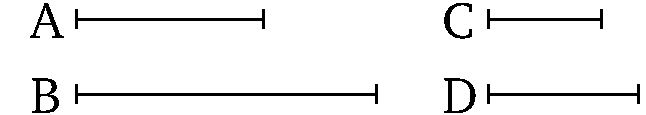
\includegraphics{Book08/fig16e.pdf}}

Let $A$ and $B$ be square numbers, and let $C$ and $D$ be their
sides (respectively). And let $A$ not measure $B$. I say that  $C$ does not measure $D$ either.

For if $C$ measures $D$ then $A$ will also measure $B$
[Prop.~8.14]. And $A$ does not measure $B$. Thus,
$C$ will not measure $D$ either.

\mbox{[}So], again,  let $C$ not measure $D$. I say that $A$ will not measure $B$
either.

For if $A$ measures $B$ then $C$ will also measure $D$ [Prop.~8.14]. And $C$ does not measure $D$.
Thus, $A$ will not measure $B$ either. (Which is) the very thing it was required to show.}
\end{Parallel}

%%%%%%
% Prop 8.17
%%%%%%
\pdfbookmark[1]{Proposition 8.17}{pdf8.17}
\begin{Parallel}{}{} 
\ParallelLText{
\begin{center}
{\large \ggn{17}.}
\end{center}\vspace*{-7pt}

\gr{Ἐὰν κύβοξ ἀριθμὸξ κύβον ἀριθμὸν μ\kern -.7pt  ὴ μετρῆ|, οὐδὲ ἡ
πλευρὰ τὴν πλευρὰν μετρήσει; κ>ὰν ἡ πλευρὰ τὴν πλευρὰν
μ\kern -.7pt  ὴ μετρῆ|, οὐδὲ ὁ κύβοξ τὸν κύβον μετρήσει.}\\~\\

% Removed epsf size command
\centerline{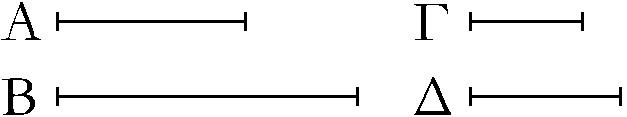
\includegraphics{Book08/fig16g.pdf}}

\gr{Κύβοξ γὰρ ἀριθμὸξ ὁ Α κύβον ἀριθμὸν τὸν Β
μ\kern -.7pt  ὴ μετρείτω, καὶ τοῦ μὲν Α πλευρὰ >έστω ὁ Γ, τοῦ
δὲ Β ὁ Δ; λέγω, <ότι ὁ Γ τὸν Δ οὐ μετρήσει.}

\gr{Εἰ γὰρ μετρεῖ ὁ Γ τὸν Δ, καὶ ὁ Α τὸν Β μετρήσει. οὐ μετρεῖ
δὲ ὁ Α τὸν Β; οὐδ> >άρα ὁ Γ  τὸν Δ μετρεῖ.}

\gr{Ἀλλὰ δὴ μ\kern -.7pt  ὴ μετρείτω ὁ Γ τὸν Δ; λέγω, <ότι οὐδὲ ὁ
Α τὸν Β μετρήσει.}

\gr{Εἰ γὰρ ὁ Α τὸν Β μετρεῖ, καὶ ὁ Γ τὸν Δ μετρήσει. οὐ μετρεῖ
δὲ ὁ Γ τὸν Δ; οὐδ> >άρα ὁ Α τὸν Β μετρήσει; <όπερ
>έδει δεῖχαι.}}

\ParallelRText{
\begin{center}
{\large Proposition 17}
\end{center}

If a cube number does not measure a(nother)
cube number then  the side (of the former) will not  measure the
side (of the latter) either. And if the side (of a cube number) does not measure the
side (of another cube number) then the (former)
cube (number) will not measure the (latter) cube (number) either.

% Removed epsf size command
\centerline{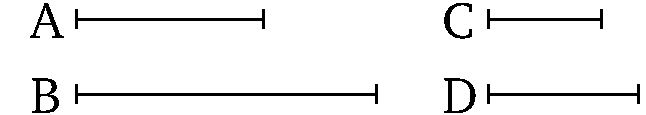
\includegraphics{Book08/fig16e.pdf}}

For let the cube number $A$ not measure the cube number $B$.
And let $C$ be the side of $A$, and $D$ (the side) of $B$.
I say that  $C$ will not measure $D$.

For if $C$ measures $D$ then $A$ will also measure $B$
[Prop.~8.15]. And $A$ does not measure $B$. Thus,
$C$ does not measure $D$ either.

And so let $C$ not measure $D$. I say that $A$ will not measure $B$
either.

For if $A$ measures $B$ then $C$ will also measure $D$ [Prop.~8.15]. And $C$ does not measure $D$.
Thus, $A$ will not measure $B$ either. (Which is) the very thing it was required to show.}
\end{Parallel}

%%%%%%
% Prop 8.18
%%%%%%
\pdfbookmark[1]{Proposition 8.18}{pdf8.18}
\begin{Parallel}{}{} 
\ParallelLText{
\begin{center}
{\large \ggn{18}.}
\end{center}\vspace*{-7pt}

\gr{Δύο ὁμοίων ἐπιπέδων ἀριθμῶν ε<ῖξ μέσοξ
ἀνάλογόν ἐστιν ἀριθμόξ; καὶ ὁ ἐπίπεδοξ πρὸξ τὸν
ἐπίπεδον διπλασίονα λόγον >έθει >ήπερ ἡ ὁμόλογοξ πλευρὰ
πρὸξ τὴν ὁμόλογον πλευράν.}\\~\\

% Removed epsf size command
\centerline{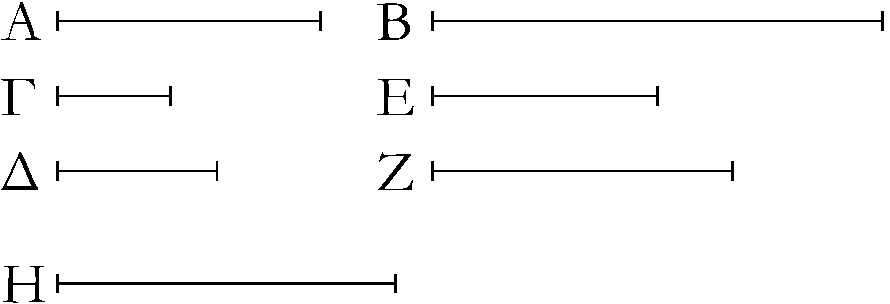
\includegraphics{Book08/fig18g.pdf}}

\gr{>'Εστωσαν δύο <όμοιοι ἐπίπεδοι ἀριθμοὶ οἱ Α, Β, καὶ τοῦ
μὲν Α πλευραὶ >έστωσαν οἱ Γ, Δ ἀριθμοί, τοῦ δὲ Β οἱ Ε, Ζ. καὶ
ἐπεὶ <όμοιοι ἐπίπεδοί εἰσιν οἱ ἀνάλογον >έθοντεξ τὰξ πλευράξ,
>έστιν >άρα ὡξ ὁ Γ πρὸξ τὸν Δ, ο<ύτωξ ὁ Ε πρὸξ τὸν Ζ. λέγω
ο>ῦν, <ότι τῶν Α, Β ε<ῖξ μέσοξ ἀνάλογόν ἐστιν ἀριθμόξ,
καὶ ὁ Α πρὸξ τὸν Β διπλασίονα λόγον >έθει >ήπερ ὁ Γ πρὸξ
τὸν Ε >ὴ ὁ Δ πρὸξ τὸν Ζ, τουτέστιν >ήπερ ἡ ὁμόλογοξ
πλευρὰ πρὸξ τὴν ὁμόλογον [πλευράν].}

\gr{Καὶ ἐπεί ἐστιν ὡξ ὁ Γ πρὸξ τὸν Δ, ο<ύτωξ ὁ Ε
πρὸξ τὸν Ζ, ἐναλλὰχ >άρα ἐστὶν ὡξ ὁ Γ πρὸξ τὸν
Ε, ὁ Δ πρὸξ τὸν Ζ. καὶ ἐπεὶ ἐπίπεδόξ ἐστιν ὁ Α,
πλευραὶ δὲ α\kern -.7pt  ὐτοῦ οἱ Γ, Δ, ὁ Δ >άρα τὸν Γ πολλαπλασιάσαξ τὸν Α
πεποίηκεν. διὰ τὰ α\kern -.7pt  ὐτὰ δὴ καὶ ὁ Ε τὸν Ζ πολλαπλασιάσαξ τὸν Β
πεποίηκεν. ὁ Δ δὴ τὸν Ε πολλαπλασιάσαξ τὸν Η ποιείτω. καὶ
ἐπεὶ ὁ Δ τὸν μὲν Γ πολλαπλασιάσαξ τὸν Α πεποίηκεν,
τὸν δὲ Ε πολλαπλασιάσαξ τὸν 
Η πεποίηκεν, >έστιν >άρα ὡξ ὁ Γ πρὸξ τὸν Ε, ο<ύτωξ ὁ
Α πρὸξ τὸν Η. ἀλλ> ὡξ ὁ Γ πρὸξ τὸν Ε, [ο<ύτωξ]
ὁ Δ πρὸξ τὸν Ζ; καὶ ὡξ >άρα ὁ Δ πρὸξ τὸν Ζ, ο<ύτωξ
ὁ Α πρὸξ τὸν Η. πάλιν, ἐπεὶ ὁ Ε τὸν μὲν Δ πολλαπλασιάσαξ
τὸν Η πεποίηκεν, τὸν δὲ Ζ πολλαπλασιάσαξ τὸν Β πεποίηκεν,
>έστιν >άρα ὡξ ὁ Δ πρὸξ τὸν Ζ, ο<ύτωξ ὁ Η πρὸξ τὸν Β.
ἐδείθθη δὲ καὶ ὡξ ὁ Δ πρὸξ τὸν Ζ, ο<ύτωξ ὁ Α πρὸξ τὸν Η; καὶ
ὡξ >άρα ὁ Α πρὸξ τὸν Η, ο<ύτωξ ὁ Η πρὸξ τὸν Β.
οἱ Α, Η, Β >άρα ἑχῆξ ἀνάλογόν εἰσιν. τῶν Α, Β >άρα ε<ῖξ
μέσοξ ἀνάλογόν ἐστιν ἀριθμόξ.}

\gr{Λέγω δή, <ότι καὶ ὁ Α πρὸξ τὸν Β διπλασίονα λόγον >έθει >ήπερ
ἡ ὁμόλογοξ πλευρὰ πρὸξ τὴν ὁμόλογον πλευράν, τουτέστιν
>ήπερ ὁ Γ πρὸξ τὸν Ε >ὴ ὁ Δ πρὸξ τὸν Ζ. ἐπεὶ γὰρ οἱ Α, Η, Β
ἑχῆξ ἀνάλογόν εἰσιν, ὁ Α πρὸξ τὸν Β διπλασίονα
λόγον >έθει >ήπερ πρὸξ τὸν Η. καί ἐστιν ὡξ ὁ Α πρὸξ τὸν Η,
ο<ύτωξ <ό τε Γ πρὸξ τὸν Ε καὶ ὁ Δ πρὸξ τὸν Ζ.
καὶ ὁ Α >άρα  πρὸξ τὸν Β διπλασίονα λόγον >έθει >ήπερ
ὁ Γ πρὸξ τὸν Ε >ὴ ὁ Δ πρὸξ τὸν Ζ; <όπερ >έδει δεῖχαι.}}

\ParallelRText{
\begin{center}
{\large Proposition 18}
\end{center}

There exists one number in mean proportion to
two similar plane numbers. And (one) plane (number)
has to the (other) plane (number) a squared$^\dag$ ratio with respect to (that)
a corresponding side (of the former has) to a corresponding side (of the latter).

% Removed epsf size command
\centerline{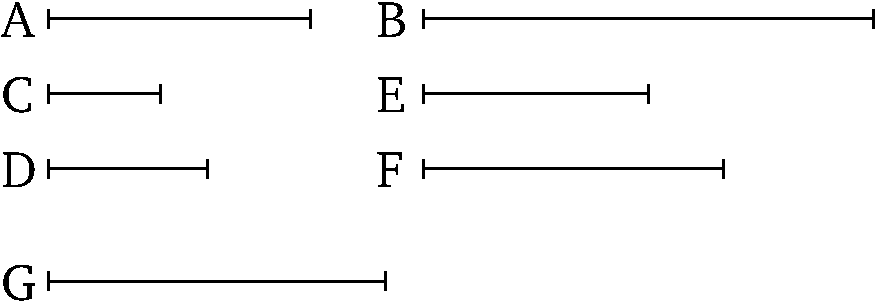
\includegraphics{Book08/fig18e.pdf}}

Let $A$ and $B$ be two similar plane numbers. And let the numbers $C$, $D$ be the
sides of $A$, and $E$, $F$ (the sides) of $B$. And since similar
numbers are those having proportional sides [Def.~7.21], thus as $C$ is to $D$, so
$E$ (is) to $F$. Therefore, I say that there exists one number in mean proportion
to $A$ and $B$, and that $A$ has to $B$ a squared ratio with
respect to that $C$ (has) to $E$, or $D$ to $F$---that is to say, with respect to
(that) a
corresponding side (has) to a corresponding [side].

For since as $C$ is to $D$, so $E$ (is) to $F$, thus, alternately, 
as $C$ is to $E$, so $D$ (is) to $F$ [Prop.~7.13].
And since $A$ is  plane, and $C$, $D$ its sides, $D$ has
thus made $A$ (by) multiplying $C$. And so, for the same (reasons),
$E$ has made $B$ (by) multiplying $F$.  So let $D$ make
$G$ (by) multiplying $E$. And since $D$ has made $A$ (by) multiplying
$C$, and has made $G$ (by) multiplying $E$, thus as $C$ is to
$E$, so $A$ (is) to $G$ [Prop.~7.17].
But as $C$ (is) to $E$, [so] $D$ (is) to $F$. And thus as $D$ (is) to  $F$,
so $A$ (is) to $G$. Again, since $E$ has made $G$ (by) multiplying
$D$, and has made $B$ (by) multiplying $F$, thus as $D$ is to $F$, so
$G$ (is) to $B$ [Prop.~7.17]. And it was
also shown that as $D$ (is) to $F$, so $A$ (is) to $G$. And thus as 
$A$ (is) to $G$, so $G$ (is) to $B$.  Thus, $A$, $G$, $B$ are continously
proportional. Thus, there exists one number (namely, $G$) in mean proportion to $A$ and $B$.

So I say that $A$ also has to $B$ a squared ratio with respect to (that)
a corresponding side (has) to a corresponding side---that is to say, with respect to (that) $C$ (has) to $E$, or $D$ to $F$. For since $A$, $G$, $B$
are continuously proportional, $A$ has to $B$ a squared ratio
with respect to (that $A$ has) to $G$ [Prop.~5.9].
And  as $A$ is to $G$, so $C$ (is) to $E$, and $D$ to $F$.
And thus $A$ has to $B$ a squared ratio with respect to (that)
$C$ (has) to $E$, or $D$ to $F$. (Which is) the very thing it was required to
show.}
\end{Parallel}
{\footnotesize\noindent$^\dag$  Literally, ``double''.}

%%%%%%
% Prop 8.19
%%%%%%
\pdfbookmark[1]{Proposition 8.19}{pdf8.19}
\begin{Parallel}{}{} 
\ParallelLText{
\begin{center}
{\large \ggn{19}.}
\end{center}\vspace*{-7pt}

\gr{Δύο ὁμοίων στερεῶν ἀριθμῶν δύο μέσοι ἀνάλογον ἐμπίπτουσιν
ἀριθμοί; καὶ ὁ στερεὸξ πρὸξ τὸν <όμοιον στερεὸν τριπλασίονα λόγον
>έθει >ήπερ ἡ ὁμόλογοξ πλευρὰ πρὸξ τὴν ὁμόλογον πλευράν.}

% Removed epsf size command
\centerline{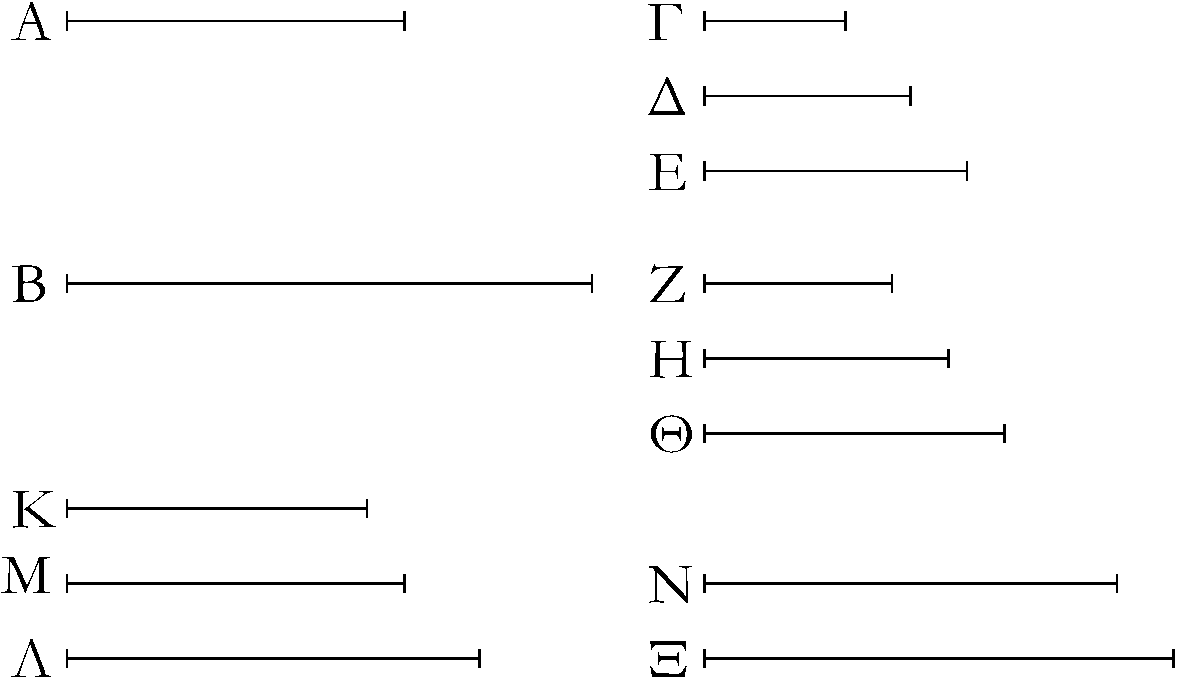
\includegraphics{Book08/fig19g.pdf}}

\gr{>'Εστωσαν δύο <όμοιοι στερεοὶ οἱ Α, Β, καὶ τοῦ μὲν Α πλευραὶ >έστωσαν οἱ Γ, Δ, Ε, τοῦ δὲ Β οἱ Ζ, Η, Θ. καὶ ἐπεὶ <όμοιοι στερεοί
εἰσιν οἱ ἀνάλογον >έθοντεξ τὰξ πλευράξ, >έστιν >άρα ὡξ μὲν
ὁ Γ πρὸξ τὸν Δ, ο<ύτωξ ὁ Ζ πρὸξ τὸν Η, ὡξ δὲ ὁ Δ πρὸξ
τὸν Ε, ο<ύτωξ ὁ Η πρὸξ τὸν Θ. λέγω, <ότι τῶν Α, Β δύο μέσοι
ἀνάλογόν ἐμπίπτουσιν ἀριθμοί, καὶ ὁ Α πρὸξ τὸν Β τριπλασίονα
λόγον >έθει >ήπερ ὁ Γ πρὸξ τὸν Ζ καὶ ὁ Δ πρὸξ τὸν Η καὶ >έτι
ὁ Ε πρὸξ τὸν Θ.}

\gr{Ὁ Γ γὰρ τὸν Δ πολλαπλασιάσαξ τὸν Κ ποιείτω, ὁ δὲ Ζ τὸν Η
πολλαπλασιάσαξ τὸν Λ ποιείτω. καὶ  ἐπεὶ οἱ Γ, Δ τοὶξ Ζ, Η ἐν τῶ| α\kern -.7pt  ὐτῶ| λόγῳ εἰσίν, καὶ ἐκ μὲν τῶν Γ, Δ ἐστιν ὁ Κ, ἐκ δὲ τῶν
Ζ, Η ὁ Λ, οἱ Κ, Λ [>άρα] <όμοιοι ἐπίπεδοί εἰσιν ἀριθμοί; τῶν Κ,
Λ >άρα ε<ῖξ μέσοξ ἀνάλογόν ἐστιν ἀριθμόξ. >έστω ὁ Μ.
ὁ Μ >άρα ἐστὶν ὁ ἐκ τῶν Δ, Ζ, ὡξ ἐν τῶ| πρὸ τούτου
θεωρήματι ἐδείθθη. καὶ ἐπεὶ ὁ Δ τὸν μὲν Γ πολλαπλασιάσαξ τὸν Κ
πεποίηκεν, τὸν δὲ Ζ πολλαπλασιάσαξ τὸν Μ πεποίηκεν, >έστιν
>άρα ὡξ ὁ Γ πρὸξ τὸν Ζ, ο<ύτωξ ὁ Κ πρὸξ τὸν Μ. ἀλλ> ὡξ
ὁ Κ πρὸξ τὸν Μ, ὁ Μ πρὸξ τὸν Λ. οἱ Κ, Μ, Λ >άρα ἑχῆξ εἰσιν ἀνάλογον ἐν τῶ| τοῦ Γ πρὸξ τὸν Ζ λόγῶ|. καὶ ἐπεί ἐστιν ὡξ
ὁ Γ πρὸξ τὸν Δ, ο<ύτωξ ὁ Ζ πρὸξ τὸν Η, ἐναλλὰχ >άρα ἐστὶν ὡξ ὁ
Γ πρὸξ τὸν Ζ, ο<ύτωξ ὁ Δ πρὸξ τὸν Η.
διὰ τὰ α\kern -.7pt  ὐτὰ δὴ καὶ ὡξ ὁ Δ πρὸξ τὸν Η,
ο<ύτωξ ὁ Ε πρὸξ τὸν Θ.
οἱ Κ, Μ, Λ >άρα ἑχῆξ εἰσιν ἀνάλογον >έν τε τῶ| τοῦ Γ πρὸξ
τὸν Ζ λόγῳ καὶ τῶ| τοῦ Δ πρὸξ τὸν Η καὶ >έτι τῶ| τοῦ Ε
πρὸξ τὸν Θ. ἑκατεροξ δὴ τῶν Ε, Θ τὸν Μ πολλαπλασιάσαξ
 ἑκάτερον τῶν Ν, Χ ποιείτω. καὶ ἐπεὶ στερεόξ ἐστιν ὁ Α,
πλευραὶ δὲ α\kern -.5pt  ὐτοῦ εἰσιν οἱ Γ, Δ, Ε, ὁ Ε >άρα τὸν ἐκ τῶν Γ, Δ
πολλαπλασιάσαξ τὸν Α πεποίηκεν. ὁ δὲ ἐκ τῶν Γ, Δ 
ἐστιν ὁ Κ; ὁ Ε >άρα τὸν Κ
πολλαπλασιάσαξ τὸν Α
πεποίηκεν. διὰ τὰ α\kern -.3pt  ὐτὰ δὴ καὶ ὁ Θ τὸν Λ 
πολλαπλασιάσαξ τὸν Β πεποίηκεν. καὶ ἐπεὶ ὁ
Ε τὸν Κ πολλαπλασιάσαξ τὸν Α πεποίηκεν,
 ἀλλὰ μ\kern -.7pt  ὴν καὶ τὸν Μ πολλαπλασιάσαξ
τὸν Ν πεποίηκεν, >έστιν >άρα ὡξ ὁ Κ πρὸξ τὸν Μ, ο<ύτωξ
ὁ Α πρὸξ τὸν Ν. ὡξ δὲ ὁ Κ πρὸξ τὸν Μ, ο<ύτωξ
<ό τε Γ πρὸξ τὸν Ζ καὶ ὁ Δ πρὸξ τὸν Η  καὶ >έτι ὁ Ε πρὸξ τὸν Θ;
καὶ ὡξ >άρα ὁ  Γ
πρὸξ τὸν Ζ καὶ ὁ Δ πρὸξ τὸν Η καὶ ὁ Ε πρὸξ
τὸν Θ, ο<ύτωξ ὁ Α πρὸξ τὸν Ν. πάλιν, ἐπεὶ ἑκάτεροξ τῶν Ε, Θ
τὸν Μ πολλαπλασιάσαξ ἑκάτερον τῶν Ν, Χ πεποίηκεν, >έστιν >άρα ὡξ ὁ Ε πρὸξ τὸν Θ, ο<ύτωξ ὁ Ν πρὸξ τὸν Χ. ἀλλ> ὡξ ὁ Ε πρὸξ τὸν Θ, ο<ύτωξ <ό τε Γ πρὸξ τὸν Ζ καὶ ὁ Δ πρὸξ τὸν  Η; καὶ ὡξ
>άρα ὁ Γ πρὸξ τὸν Ζ καὶ ὁ Δ πρὸξ τὸν Η καὶ ὁ Ε πρὸξ τὸν Θ, ο<ύτωξ
<ό τε Α πρὸξ τὸν Ν καὶ ὁ Ν πρὸξ τὸν Χ. πάλιν, ἐπεὶ ὁ Θ τὸν Μ
πολλαπλασιάσαξ τὸν Χ πεποίηκεν, ἀλλὰ μ\kern -.7pt  ὴν καὶ τὸν Λ πολλαπλασιάσαξ
τὸν Β πεποίηκεν, >έστιν >άρα ὡξ ὁ Μ πρὸξ τὸν Λ, ο<ύτωξ
ὁ Χ πρὸξ τὸν Β. ἀλλ> ὡξ ὁ Μ πρὸξ τὸν Λ, ο<ύτωξ <ό τε Γ πρὸξ τὸν
Ζ καὶ ὁ Δ πρὸξ τὸν Η καὶ ὁ Ε πρὸξ τὸν Θ. καὶ ὡξ >άρα ὁ Γ πρὸξ τὸν Ζ καὶ ὁ Δ πρὸξ τὸν Η καὶ ὁ Ε πρὸξ τὸν Θ, ο<ύτωξ οὐ
μόνον ὁ Χ πρὸξ τὸν Β, ἀλλὰ καὶ ὁ Α πρὸξ τὸν Ν καὶ  ὁ Ν πρὸξ
τὸν Χ. οἱ Α, Ν, Χ, Β >άρα ἑχῆξ εἰσιν ἀνάλογον ἐν τοῖξ
εἰρημένοιξ τῶν πλευρῶν λόγοιξ.}

\gr{Λέγω, <ότι καὶ ὁ Α πρὸξ τὸν Β τριπλασίονα λόγον >έθει
>ήπερ ἡ ὁμόλογοξ πλευρὰ πρὸξ τὴν ὁμόλογον πλευράν, τουτέστιν
>ήπερ ὁ Γ ἀριθμὸξ πρὸξ τὸν Ζ >ὴ ὁ Δ πρὸξ τὸν Η καὶ >έτι
ὁ Ε πρὸξ τὸν Θ. ἐπεὶ γὰρ τέσσαρεξ ἀριθμοὶ ἑχῆξ ἀνάλογόν εἰσιν
οἱ Α, Ν, Χ, Β, ὁ Α >άρα πρὸξ τὸν Β τριπλασίονα λόγον >έθει >ήπερ
ὁ Α πρὸξ τὸν Ν. ἀλλ> ὡξ ὁ Α πρὸξ τὸν Ν, ο<ύτωξ ἐδείθθη
<ό τε Γ πρὸξ τὸν Ζ καὶ ὁ Δ πρὸξ τὸν Η καὶ >έτι ὁ Ε πρὸξ
τὸν Θ. καὶ ὁ Α >άρα πρὸξ τὸν  Β τριπλασίονα λόγον >έθει >ήπερ
ἡ ομόλογοξ πλευρὰ πρὸξ τὴν ὁμόλογον πλευράν, τουτέστιν
>ήπερ ὁ Γ ἀριθμὸξ πρὸξ τὸν Ζ καὶ ὁ Δ πρὸξ τὸν Η καὶ >έτι ὁ Ε πρὸξ τὸν Θ;  <όπερ >έδει δεῖχαι.}}

\ParallelRText{
\begin{center}
{\large Proposition 19}
\end{center}

Two numbers fall (between)
two similar solid numbers in mean proportion. And a solid (number) has to a similar solid (number) a cubed$^\dag$ ratio with respect to
(that) a corresponding side (has) to a corresponding side.

% Removed epsf size command
\centerline{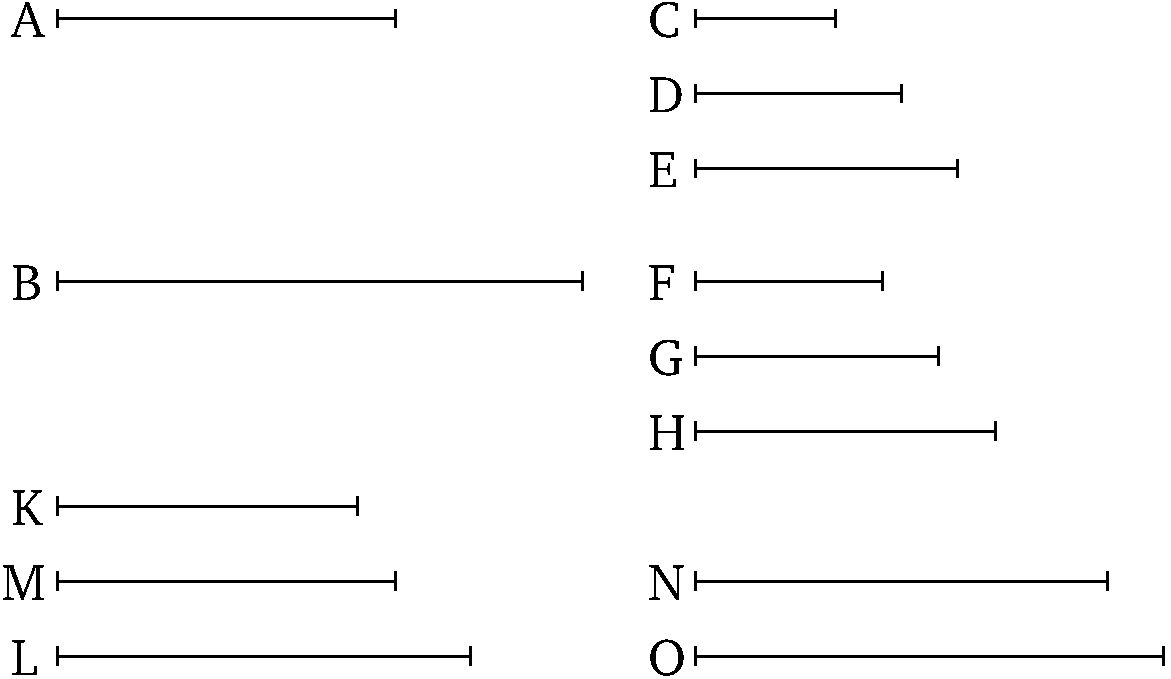
\includegraphics{Book08/fig19e.pdf}}

Let $A$ and $B$ be two similar solid numbers, and let $C$, $D$, $E$ be the sides of $A$, and $F$, $G$, $H$ (the sides) of $B$. And
since similar solid (numbers) are those having proportional sides [Def.~7.21], thus as $C$ is to $D$, so $F$
(is) to $G$, and as $D$ (is) to $E$, so $G$ (is) to $H$. I say that two
numbers  fall  (between) $A$ and $B$ in mean proportion, and (that) $A$
has to $B$ a cubed ratio with respect to (that) $C$ (has) to $F$, and
$D$ to $G$, and, further, $E$ to $H$.

For let $C$ make $K$ (by) multiplying $D$, and let $F$ make $L$
(by) multiplying $G$. And since $C$, $D$ are in the same ratio as $F$, $G$,
and $K$ is the (number created) from (multiplying) $C$, $D$, and $L$ the (number created) from
(multiplying) $F$, $G$, [thus] $K$ and $L$ are  similar plane numbers [Def.~7.21]. Thus, there exits one number
in mean proportion to $K$ and $L$ [Prop.~8.18].
Let it be $M$. Thus, $M$ is the (number created) from (multiplying) $D$, $F$, as shown in the theorem before this (one). And since $D$ has made $K$ (by) multiplying $C$, and has made $M$ (by) multiplying $F$, thus as $C$ is to $F$, so
$K$ (is) to $M$ [Prop.~7.17]. But, as $K$ (is) to $M$, (so) $M$ (is) to $L$. Thus, $K$, $M$, $L$ are continuously
proportional in the ratio of $C$ to $F$. And since as $C$ is to $D$, so $F$
(is) to $G$, thus, alternately, as $C$ is to $F$, so $D$ (is) to $G$ [Prop.~7.13]. And so, for the same (reasons), 
as $D$ (is) to $G$, so $E$ (is) to $H$. Thus, $K$, $M$, $L$ are continuously
proportional in the ratio of $C$ to $F$, and of $D$ to $G$, and, further,  of $E$ to $H$. So let  $E$, $H$ make  $N$, $O$, respectively, (by) multiplying $M$. And since $A$ is  solid, and $C$, $D$, $E$ are its sides, $E$ has thus made $A$ (by) multiplying the (number created) from
(multiplying) $C$, $D$. And  $K$ 
is the (number created) from (multiplying)
$C$, $D$. Thus, $E$ has made $A$ (by) multiplying $K$. And so, for the
same (reasons), $H$ has made $B$ (by) multiplying $L$. And since
$E$ has made $A$ (by) multiplying $K$, but has, in fact, also made $N$ (by)
multiplying $M$, thus as $K$ is to $M$, so $A$ (is) to $N$ [Prop.~7.17].  And as $K$ (is) to $M$, so
$C$ (is) to $F$, and $D$ to $G$, and, further, $E$ to $H$. And thus as $C$
(is) to $F$, and $D$ to $G$, and $E$ to $H$, so $A$ (is) to $N$. Again, since
 $E$, $H$ have made  $N$, $O$, respectively, (by) multiplying $M$,
thus as $E$ is to $H$, so $N$ (is) to $O$ [Prop.~7.18]. But, as $E$ (is) to $H$, so $C$
(is) to $F$, and $D$ to $G$.  And thus as $C$ (is) to $F$, and $D$ to $G$,
and $E$ to $H$, so (is) $A$ to $N$, and $N$ to $O$. Again, since
$H$ has made $O$ (by) multiplying $M$, but  has, in fact, also made
$B$ (by) multiplying $L$, thus as $M$ (is) to $L$, so $O$ (is) to $B$ [Prop.~7.17]. But, as $M$ (is) to $L$, so $C$ (is)
to $F$, and $D$ to $G$, and $E$ to $H$. And thus as $C$ (is) to $F$,
and $D$ to $G$, and $E$ to $H$, so not only (is) $O$ to $B$, but
also $A$ to $N$, and $N$ to $O$. Thus,	 $A$, $N$, $O$, $B$ are continuously proportional in the aforementioned ratios of the sides.

So I say that $A$ also has to $B$ a cubed ratio with respect to (that)
a corresponding side (has) to a corresponding side---that is to say, with respect to (that) the number $C$ (has) to $F$, or $D$ to $G$, and, further,  $E$ to $H$. For
since $A$, $N$, $O$, $B$ are four continuously proportional numbers,
$A$ thus has to $B$	a cubed ratio with respect to (that) $A$ (has)
to $N$ [Def.~5.10]. But, as $A$ (is) to $N$, so
it was shown (is) $C$ to $F$, and $D$ to $G$, and, further, $E$ to $H$. And thus $A$ has to $B$ a cubed ratio with respect to (that) a corresponding
side (has) to a corresponding side---that is to say, with respect to
(that) the number $C$ (has) to $F$, and $D$ to $G$, and, further, $E$ to
$H$. (Which is) the very thing it was required to show.}
\end{Parallel}
{\footnotesize\noindent$^\dag$  Literally, ``triple''.}

%%%%%%
% Prop 8.20
%%%%%%
\pdfbookmark[1]{Proposition 8.20}{pdf8.20}
\begin{Parallel}{}{} 
\ParallelLText{
\begin{center}
{\large \ggn{20}.}
\end{center}\vspace*{-7pt}

\gr{Ἐὰν δύο ἀριθμῶν ε<ῖξ μέσοξ  ἀνάλογον ἐμπίπτῆ| ἀριθμόξ,
<όμοιοι ἐπίπεδοι >έσονται οἱ ἀριθμοί.}

\gr{Δύο γὰρ ἀριθμῶν τῶν Α, Β ε<ῖξ μέσοξ ἀνάλογον ἐμπιπτέτω ἀριθμὸξ ὁ Γ; λέγω, <ότι οἱ Α, Β <όμοιοι ἐπίπεδοί εἰσιν ἀριθμοί.}\\

% Removed epsf size command
\centerline{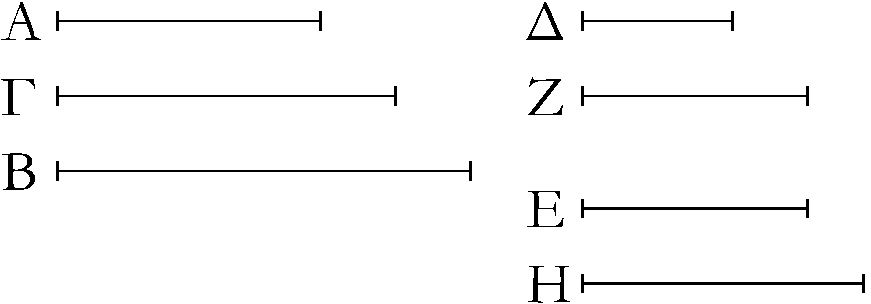
\includegraphics{Book08/fig20g.pdf}}

\gr{Εἰλήφθωσαν [γὰρ] ἐλάθιστοι ἀριθμοὶ τῶν τὸν α\kern -.7pt  ὐτὸν λόγον
ἐθόντων τοῖξ Α, Γ οἱ Δ, Ε; ἰσάκιξ >άρα ὁ Δ τὸν Α μετρεῖ καὶ
ὁ Ε τὸν Γ.  ὁσάκιξ
δὴ ὁ Δ τὸν Α μετρεῖ, τοσα\kern -.7pt  ῦται μονάδεξ >έστωσαν ἐν τῶ| Ζ; ὁ Ζ >άρα τὸν Δ
πολλαπλασιάσαξ τὸν Α πεποίηκεν. <ώστε ὁ Α ἐπίπεδόξ ἐστιν, πλευραὶ
δὲ α\kern -.5pt  ὐτοῦ οἱ Δ, Ζ. πάλιν, ἐπεὶ οἱ Δ, Ε ἐλάθιστοί εἰσι τῶν τὸν
α\kern -.3pt  ὐτὸν λόγον ἐθόντων τοῖξ Γ, Β, ἰσάκιξ >άρα ὁ Δ τὸν Γ
μετρεῖ καὶ ὁ Ε τὸν Β. ὁσάκιξ δὴ ὁ Ε τὸν Β μετρεῖ, τοσα\kern -.7pt  ῦται
μονάδεξ >έστωσαν ἐν τῶ| Η. ὁ Ε >άρα τὸν Β μετρεῖ κατὰ τὰξ
ἐν τῶ| Η μονάδαξ; ὁ Η >άρα τὸν Ε πολλαπλασιάσαξ τὸν Β πεποίηκεν.
ὁ Β >άρα  ἐπίπεδοξ ἐστι, πλευραὶ δὲ α\kern -.7pt  ὐτοῦ εἰσιν οἱ Ε, Η.
οἱ Α, Β >άρα ἐπίπεδοί εἰσιν ἀριθμοί. λέγω δή, <ότι
καὶ <όμοιοι. ἐπεὶ γὰρ ὁ Ζ τὸν μὲν Δ πολλαπλασιάσαξ τὸν
Α πεποίηκεν, τὸν δὲ Ε πολλαπλασιάσαξ τὸν Γ πεποίηκεν, >έστιν >άρα
ὡξ ὁ Δ πρὸξ τὸν Ε, ο<ύτωξ ὁ Α πρὸξ τὸν Γ, τουτέστιν
ὁ Γ πρὸξ τὸν Β. πάλιν, ἐπεὶ ὁ Ε ἑκάτερον τῶν Ζ, Η πολλαπλασιάσαξ 
τοὺξ Γ, Β πεποίηκεν, >έστιν >άρα ὡξ ὁ Ζ πρὸξ τὸν Η, ο<ύτωξ
ὁ Γ πρὸξ τὸν Β. ὡξ δὲ ὁ Γ πρὸξ τὸν Β, ο<ύτωξ
ὁ Δ πρὸξ τὸν Ε; καὶ ὡξ >άρα ὁ Δ πρὸξ τὸν  Ε, ο<ύτωξ
ὁ Ζ πρὸξ τὸν Η; καὶ ἐναλλὰχ ὡξ ὁ Δ πρὸξ τὸν Ζ, ο<ύτωξ ὁ Ε
πρὸξ τὸν Η. οἱ Α, Β >άρα <όμοιοι ἐπίπεδοι ἀριθμοί εἰσιν; αἱ γὰρ
πλευραὶ α\kern -.7pt  ὐτῶν ἀνάλογόν εἰσιν; <όπερ >έδει δεῖχαι.}}

\ParallelRText{
\begin{center}
{\large Proposition 20}
\end{center}

If one number falls between two
numbers in mean proportion then the numbers will be similar plane (numbers).

For let one number $C$ fall  between the two numbers $A$
and $B$ in mean proportion. I say that $A$ and $B$ are similar plane numbers.

% Removed epsf size command
\centerline{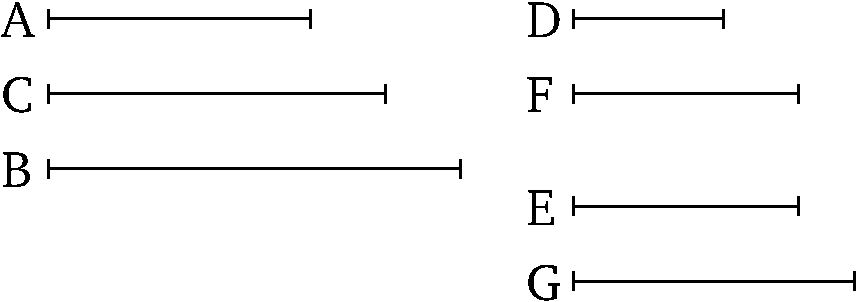
\includegraphics{Book08/fig20e.pdf}}

\mbox{[}For] let the least numbers, $D$ and $E$,  having the same ratio as $A$ and $C$ be taken [Prop.~7.33]. Thus,
$D$ measures $A$ as many  times as  $E$ (measures) $C$
[Prop.~7.20]. So as many times as $D$ measures $A$, so many units let there be in $F$. Thus, $F$ has made $A$ (by)
multiplying $D$ [Def.~7.15]. Hence, $A$ is 
plane, and $D$, $F$ (are) its sides. Again, since $D$ and $E$
are the least of those (numbers) having  the same ratio as $C$ and $B$, 
$D$ thus measures $C$ as many times as $E$ (measures) $B$ [Prop.~7.20]. So as many times as $E$ measures
$B$, so many units let there be in $G$. Thus, $E$ measures $B$ according to
the units in $G$. Thus, $G$ has made $B$ (by) multiplying $E$ [Def.~7.15]. Thus, $B$ is plane, and $E$, $G$ are its sides. Thus, $A$ and $B$ are (both) plane numbers. So I say that
(they are) also similar. For since $F$ has made $A$ (by) multiplying $D$,
and has made $C$ (by) multiplying $E$, thus as $D$ is to $E$, so $A$ (is) to $C$---that is to say, $C$ to $B$ [Prop.~7.17].$^\dag$ Again, since $E$ has made  $C$, $B$ (by)
multiplying  $F$, $G$, respectively, thus as $F$ is to $G$, so $C$ (is) to
$B$ [Prop.~7.17]. And as $C$ (is) to $B$, so
$D$ (is) to $E$. And thus as $D$ (is) to $E$, so $F$ (is) to $G$. And,
alternately, as $D$ (is) to $F$, so $E$ (is) to $G$ [Prop.~7.13]. Thus, $A$ and $B$ are similar plane
numbers. For their sides are proportional [Def.~7.21].
(Which is) the very thing it was required to show.}
\end{Parallel}
{\footnotesize\noindent$^\dag$ This part of the proof is defective, since it is not demonstrated that $F\times E = C$. Furthermore, it is
not necessary to show that $D:E::A:C$, because this
is true by hypothesis.}

%%%%%%
% Prop 8.21
%%%%%%
\pdfbookmark[1]{Proposition 8.21}{pdf8.21}
\begin{Parallel}{}{} 
\ParallelLText{
\begin{center}
{\large\ggn{21}.}
\end{center}\vspace*{-7pt}

\gr{Ἐὰν δύο ἀριθμῶν δύο μέσοι ἀνάλογον ἐμπίπτωσιν
ἀριθμοί, <όμοιοι στερεοί εἰσιν οἱ ἀριθμοί.}

\gr{Δύο γὰρ ἀριθμῶν τῶν Α, Β δύο μέσοι ἀνάλογον ἐμπιπτέτωσαν
ἀριθμοὶ οἱ Γ, Δ; λέγω, <ότι οἱ Α, Β <όμοιοι στερεοί εἰσιν.}

\gr{Εἰλήφθωσαν γὰρ ἐλάθιστοι ἀριθμοὶ τῶν τὸν α\kern -.7pt  ὐτὸν λόγον ἐθόντων
τοῖξ Α, Γ, Δ τρεῖξ οἱ Ε, Ζ, Η; οἱ >άρα >άκροι α\kern -.7pt  ὐτῶν οἱ Ε, Η
πρῶτοι πρὸξ ἀλλήλουξ εἰσίν. καὶ ἐπεὶ τῶν Ε, Η ε<ῖξ
μέσοξ ἀνάλογον ἐμπέπτωκεν ἀριθμὸξ ὁ Ζ, οἱ Ε, Η >άρα
ἀριθμοὶ <όμοιοι ἐπίπεδοί εἰσιν. >έστωσαν ο>ῦν τοῦ μὲν Ε πλευραὶ
οἱ Θ, Κ, τοῦ δὲ Η οἱ Λ, Μ. φανερὸν >άρα ἐστὶν ἐκ τοῦ πρὸ τούτου,
<ότι οἱ Ε, Ζ, Η ἑχῆξ εἰσιν ἀνάλογον >έν τε τῶ| τοῦ Θ πρὸξ τὸν Λ
λόγῳ καὶ τῶ| τοῦ Κ πρὸξ τὸν Μ. καὶ ἐπεὶ οἱ Ε, Ζ, Η ἐλάθιστοί
εἰσι τῶν τὸν α\kern -.5pt  ὐτὸν λόγον ἐθόντων τοῖξ Α, Γ, Δ, καί ἐστιν
>ίσον τὸ πλῆθοξ τῶν Ε, Ζ, Η τῶ| πλήθει τῶν Α, Γ, Δ, δι> >ίσου >άρα ἐστὶν ὡξ ὁ Ε πρὸξ τὸν Η, ο<ύτωξ ὁ Α πρὸξ τὸν Δ. οἱ δὲ Ε, Η
πρῶτοι, οἱ δὲ πρῶτοι καὶ ἐλάθιστοι, οἱ δὲ ἐλάθιστοι μετροῦσι
τοὺξ τὸν α\kern -.3pt  ὐτὸν λόγον >έθονταξ α\kern -.7pt  ὐτοῖξ ἰσάκιξ <ό τε μείζων
τὸν μείζονα καὶ ὁ ἐλάσσων τὸν ἐλάσσονα, τουτέστιν <ό
τε ἡγούμενοξ τὸν ἡγούμενον καὶ ὁ ἑπόμενοξ τὸν ἑπόμενον;
ἰσάκιξ >άρα ὁ Ε τὸν Α μετρεῖ καὶ ὁ Η τὸν Δ. ὁσάκιξ δὴ ὁ Ε
τὸν Α μετρεῖ, τοσα\kern -.7pt  ῦται μονάδεξ >έστωσαν ἐν τῶ| Ν. ὁ Ν >άρα
τὸν Ε πολλαπλασιάσαξ τὸν Α πεποίηκεν. ὁ δὲ Ε ἐστιν ὁ ἐκ τῶν Θ, Κ;
ὁ Ν >άρα τὸν ἐκ τῶν Θ, Κ πολλαπλασιάσαξ τὸν Α πεποίηκεν. στερεὸξ
>άρα ἐστὶν ὁ Α, πλευραὶ δὲ α\kern -.7pt  ὐτοῦ εἰσιν οἱ Θ, Κ, Ν. πάλιν, ἐπεὶ
οἱ Ε, Ζ, Η ἐλάθιστοί εἰσι τῶν τὸν α\kern -.7pt  ὐτὸν λόγον ἐθόντων
τοῖξ Γ, Δ, Β, ἰσάκιξ >άρα ὁ Ε τὸν Γ μετρεῖ καὶ ὁ Η τὸν Β. ὁσάκιξ
δὴ ὁ Ε τὸν Γ μετρεῖ, τοσα\kern -.7pt  ῦται μονάδεξ >έστωσαν ἐν τῶ| Χ.
ὁ Η >άρα τὸν Β μετρεῖ κατὰ τὰξ ἐν τῶ| Χ μονάδαξ; ὁ Χ
>άρα τὸν Η πολλαπλασιάσαξ τὸν Β πεποίηκεν. ὁ δὲ Η ἐστιν ὁ ἐκ
τῶν Λ, Μ; ὁ Χ >άρα τὸν ἐκ τῶν Λ, Μ πολλαπλασιάσαξ τὸν Β
πεποίηκεν. στερεὸξ >άρα ἐστὶν ὁ Β, πλευραὶ δὲ α\kern -.7pt  ὐτοῦ εἰσιν
οἱ Λ, Μ, Χ; οἱ Α, Β >άρα στερεοί εἰσιν.}\\~\\~\\~\\

% Removed epsf size command
\centerline{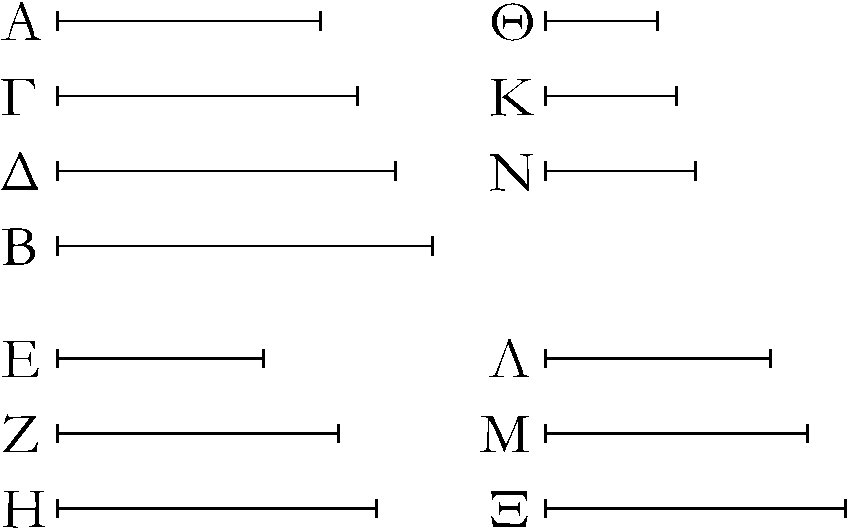
\includegraphics{Book08/fig21g.pdf}}

\gr{Λέγω [δή], <ότι καὶ <όμοιοι. ἐπεὶ γὰρ οἱ Ν, Χ τὸν Ε πολλαπλασιάσαντεξ
τοὺξ Α, Γ πεποιήκασιν, >έστιν >άρα ὡξ ὁ Ν πρὸξ τὸν Χ, ὁ Α
πρὸξ τὸν Γ, τουτέστιν ὁ Ε πρὸξ  τὸν Ζ. ἀλλ> ὡξ ὁ Ε πρὸξ τὸν Ζ, ὁ
Θ πρὸξ τὸν Λ καὶ ὁ Κ πρὸξ τὸν Μ; καὶ ὡξ >άρα ὁ Θ πρὸξ τὸν
Λ, ο<ύτωξ ὁ Κ πρὸξ τὸν Μ  καὶ ὁ Ν πρὸξ  τὸν Χ. καί εἰσιν
οἱ
 μὲν Θ, Κ, Ν πλευραὶ τοῦ Α, οἱ δὲ Χ, Λ, Μ πλευραὶ τοῦ Β. οἱ 
Α, Β >άρα ἀριθμοὶ <όμοιοι στερεοί εἰσιν; <όπερ >έδει
δεῖχαι.}}

\ParallelRText{
\begin{center}
{\large Proposition 21}
\end{center}

If two numbers fall between two numbers
in mean proportion  then the (latter) are similar solid (numbers).

For let the two numbers $C$ and $D$ fall between the two numbers
$A$ and $B$ in mean proportion. I say that $A$ and $B$ are similar
solid (numbers).

For let the three least numbers $E$, $F$, $G$  having the
same ratio as $A$, $C$, $D$ be taken [Prop.~8.2]. Thus,
the outermost of them, $E$ and $G$, are prime to one another
[Prop.~8.3]. And since one number, $F$, has
fallen (between) $E$ and $G$ in mean proportion, $E$ and $G$ are thus
similar plane numbers [Prop.~8.20].
Therefore, let $H$, $K$ be the sides of $E$, and $L$, $M$ (the sides) of $G$. Thus, it is clear from the (proposition) before this (one)
that $E$, $F$, $G$ are continuously proportional in the ratio of $H$ to $L$,
and of $K$ to $M$. And since $E$, $F$, $G$ are the least (numbers)
having the same ratio as $A$, $C$, $D$, and the multitude of $E$, $F$, $G$
is equal to the multitude of $A$, $C$, $D$, thus, via equality, as $E$ is to
$G$, so $A$ (is) to $D$ [Prop.~7.14]. And
$E$ and $G$ (are) prime (to one another), and prime (numbers) are also the least (of
those numbers having the same ratio as them) [Prop.~7.21],
and the least (numbers) measure those (numbers) having the same ratio
as them an equal number of times, the greater (measuring) the greater, and
the lesser the lesser---that is to say, the leading (measuring) the leading, and
the following the following [Prop.~7.20]. Thus,
$E$ measures $A$ the same number of times as $G$ (measures) $D$. 
So as many times as $E$ measures $A$, so many units let there be in $N$.
Thus, $N$ has made $A$ (by) multiplying $E$ [Def.~7.15]. And $E$ is the (number created) from (multiplying) $H$ and $K$. Thus, $N$ has made $A$ (by) multiplying
the (number created) from (multiplying) $H$ and $K$. Thus, $A$ is  solid, and its sides are $H$, $K$, $N$. Again, since $E$, $F$, $G$
are the least (numbers) having the same ratio as $C$, $D$, $B$, thus $E$
measures $C$ the same number of times as $G$ (measures) $B$ [Prop.~7.20]. So as many times as $E$ measures $C$, so many units let there be in $O$. Thus, $G$ measures $B$ according to
the units in $O$. Thus, $O$ has made $B$ (by) multiplying $G$. And
$G$ is the (number created) from (multiplying) $L$ and $M$. Thus, $O$ has made $B$ (by) multiplying the (number created) from (multiplying)
$L$ and $M$. Thus, $B$ is  solid, and its sides are $L$, $M$, $O$.
Thus,  $A$ and $B$ are (both) solid.

% Removed epsf size command
\centerline{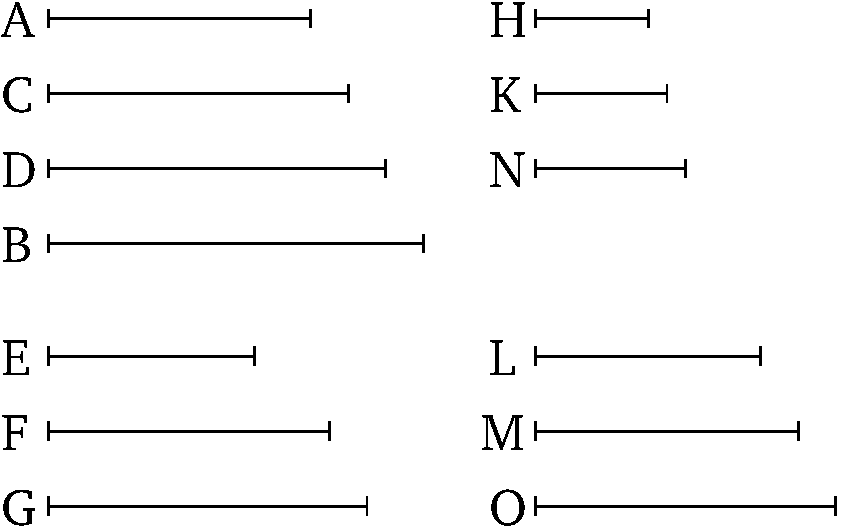
\includegraphics{Book08/fig21e.pdf}}

\mbox{[}So] I say that (they are) also similar. For since $N$, $O$ have made
$A$, $C$ (by) multiplying $E$, thus as $N$ is to $O$, so $A$ (is) to $C$---that is to say, $E$ to $F$ [Prop.~7.18]. But, as $E$
(is) to $F$, so $H$ (is) to $L$, and $K$ to $M$. And thus as $H$ (is) to $L$,
so $K$ (is) to $M$, and $N$ to $O$. And $H$, $K$, $N$
are the sides of $A$, and $L$, $M$, $O$ the sides of $B$. Thus,
$A$ and $B$ are similar solid numbers [Def.~7.21]. 
(Which is) the very thing it was required to show.}
\end{Parallel}
{\footnotesize\noindent$^\dag$ The Greek text has ``$O$, $L$, $M$'', which is obviously a mistake.}

%%%%%%
% Prop 8.22
%%%%%%
\pdfbookmark[1]{Proposition 8.22}{pdf8.22}
\begin{Parallel}{}{} 
\ParallelLText{
\begin{center}
{\large\ggn{22}.}
\end{center}\vspace*{-7pt}

\gr{Ἐὰν τρεῖξ ἀριθμοὶ ἑχῆξ ἀνάλογον >ῶσιν, ὁ δὲ πρῶτοξ
τετράγωνοξ >ῆ|, καὶ ὁ τρίτοξ τετράγωνοξ >έσται.}

\gr{>'Εστωσαν τρεῖξ ἀριθμοὶ ἑχῆξ ἀνάλογον οἱ Α, Β, Γ, ὁ δὲ
πρῶτοξ ὁ Α τετράγωνοξ >έστω; λέγω, <ότι καὶ ὁ τρίτοξ
ὁ Γ τετράγωνόξ ἐστιν.}

% Removed epsf size command
\centerline{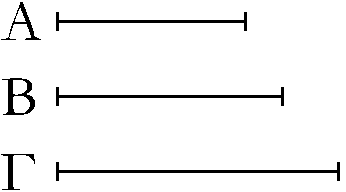
\includegraphics{Book08/fig22g.pdf}}

\gr{Ἐπεὶ γὰρ τῶν Α, Γ ε<ῖξ μέσοξ ἀνάλογόν ἐστιν
ἀριθμὸξ ὁ Β, οἱ Α, Γ >άρα <όμοιοι ἐπίπεδοί εἰσιν.
τετράγωνοξ δὲ ὁ Α; τετράγωνοξ >άρα καὶ ὁ Γ;
<όπερ >έδει δεῖχαι.}}

\ParallelRText{
\begin{center}
{\large Proposition 22}
\end{center}

If three numbers are continuously proportional,
and the first is  square, then the third will also be  square.

Let $A$, $B$, $C$ be three continuously proportional numbers, and let the
first $A$ be  square. I say that the third $C$ is also  square.

% Removed epsf size command
\centerline{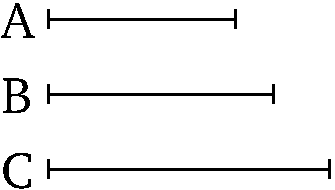
\includegraphics{Book08/fig22e.pdf}}

For since one number, $B$, is in mean proportion to $A$ and $C$, $A$
and $C$ are thus similar plane (numbers) [Prop.~8.20]. And $A$ is  square.
Thus, $C$ is also square [Def.~7.21].
(Which is) the very thing it was required to show.}
\end{Parallel}

%%%%%%
% Prop 8.23
%%%%%%
\pdfbookmark[1]{Proposition 8.23}{pdf8.23}
\begin{Parallel}{}{} 
\ParallelLText{
\begin{center}
{\large \ggn{23}.}
\end{center}\vspace*{-7pt}

\gr{Ἐὰν τέσσαρεξ ἀριθμοὶ ἑχῆξ ἀνάλογον >ῶσιν, ὁ δὲ πρῶτοξ
κύβοξ >ῆ|, καὶ ὁ τέταρτοξ κύβοξ >έσται.}

% Removed epsf size command
\centerline{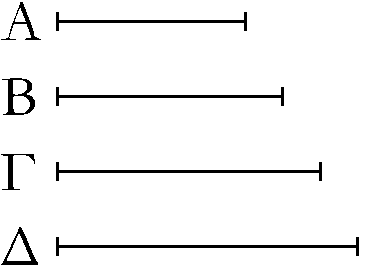
\includegraphics{Book08/fig23g.pdf}}

\gr{>'Εστωσαν τέσσαρεξ ἀριθμοὶ ἑχῆξ ἀνάλογον οἱ Α, Β, Γ, Δ, ὁ δὲ
Α κύβοξ >έστω; λέγω, <ότι καὶ ὁ Δ κύβοξ ἐστίν.}

\gr{Ἐπεὶ γὰρ τῶν Α, Δ δύο μέσοι ἀνάλογόν εἰσιν ἀριθμοὶ
οἱ Β, Γ, οἱ Α, Δ >άρα <όμοιοί εἰσι στερεοὶ ἀριθμοί. κύβοξ
δὲ ὁ Α; κύβοξ >άρα καὶ ὁ Δ; <όπερ >έδει δεῖχαι.}}

\ParallelRText{
\begin{center}
{\large Proposition 23}
\end{center}

If four numbers are continuously proportional,
and the first is  cube, then the fourth will also be cube.

% Removed epsf size command
\centerline{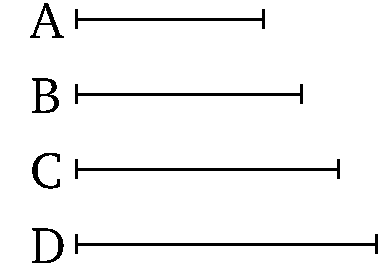
\includegraphics{Book08/fig23e.pdf}}

Let $A$, $B$, $C$, $D$ be four continuously proportional numbers, and
let $A$ be cube. I say that $D$ is also  cube.

For since two numbers, $B$ and $C$, are in mean proportion to $A$ and
$D$, $A$ and $D$ are thus similar solid numbers [Prop.~8.21]. And $A$ (is)  cube.
Thus, $D$ (is) also  cube   [Def.~7.21].
(Which is) the very thing it was required to show.}
\end{Parallel}

%%%%%%
% Prop 8.24
%%%%%%
\pdfbookmark[1]{Proposition 8.24}{pdf8.24}
\begin{Parallel}{}{} 
\ParallelLText{
\begin{center}
{\large \ggn{24}.}
\end{center}\vspace*{-7pt}

\gr{Ἐὰν δύο ἀριθμοὶ πρὸξ ἀλλήλουξ λόγον >έθωσιν, <ὸν τετράγωνοξ
ἀριθμὸξ πρὸξ τετράγωνον ἀριθμόν, ὁ δὲ πρῶτοξ τετράγωνοξ
>ῆ|, καὶ ὁ δεύτεροξ τετράγωνοξ >έσται.}

% Removed epsf size command
\centerline{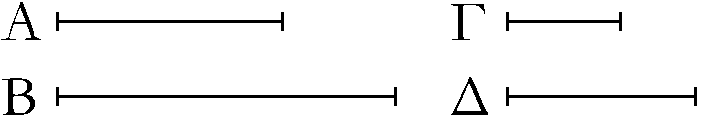
\includegraphics{Book08/fig24g.pdf}}

\gr{Δύο γὰρ ἀριθμοὶ οἱ Α, Β πρὸξ ἀλλήλουξ λόγον ἐθέτωσαν, <ὸν
τετράγωνοξ ἀριθμὸξ ὁ Γ πρὸξ τετράγωνον ἀριθμὸν τὸν Δ,
ὁ δὲ Α τετράγωνοξ >έστω; λέγω, <ότι καὶ ὁ Β τετράγωνόξ
ἐστιν.}

\gr{Ἐπεὶ γὰρ οἱ Γ, Δ τετράγωνοί εἰσιν, οἱ Γ, Δ >άρα <όμοιοι
ἐπίπεδοί εἰσιν. τῶν Γ, Δ >άρα ε~ἱξ μέσοξ ἀνάλογον ἐμπίπτει
ἀριθμόξ. καί ἐστιν ὡξ ὁ Γ πρὸξ τὸν Δ, ὁ Α πρὸξ τὸν Β; καὶ
τῶν Α, Β >άρα ε~ἱξ μέσοξ ἀνάλογον ἐμπίπτει ἀριθμόξ. καί
ἐστιν ὁ Α τετράγωνοξ; καὶ ὁ Β >άρα τετράγωνόξ ἐστιν; <όπερ
>έδει δεῖχαι.}}

\ParallelRText{
\begin{center}
{\large Proposition 24}
\end{center}

If two numbers have to one another the ratio
which a square number (has) to a(nother) square number, and
the first is  square, then the second will also be  square.

% Removed epsf size command
\centerline{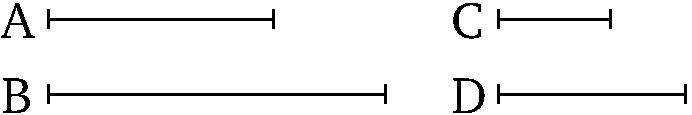
\includegraphics{Book08/fig24e.pdf}}

For let two numbers, $A$ and $B$, have to one another the ratio which
the square number $C$ (has) to the square number $D$. And let
$A$ be square. I say that $B$ is also  square.

For since $C$ and $D$ are square, $C$ and $D$ are thus
similar plane (numbers). Thus, one number falls 
(between) $C$ and $D$ in mean proportion [Prop.~8.18]. And
as $C$ is to $D$, (so) $A$ (is) to $B$. Thus, one number also
falls  (between) $A$ and $B$ in mean proportion [Prop.~8.8]. And $A$ is  square. 
Thus, $B$ is also  square [Prop.~8.22].
(Which is) the very thing it was required to show.}
\end{Parallel}

%%%%%%
% Prop 8.25
%%%%%%
\pdfbookmark[1]{Proposition 8.25}{pdf8.25}
\begin{Parallel}{}{} 
\ParallelLText{\
\begin{center}
{\large \ggn{25}.}
\end{center}\vspace*{-7pt}

\gr{Ἐὰν δύο ἀριθμοὶ πρὸξ ἀλλήλουξ λόγον >έθωσιν, <ὸν κύβοξ
ἀριθμὸξ πρὸξ κύβον ἀριθμόν, ὁ δὲ πρῶτοξ κύβοξ >ῆ|, καὶ
ὁ δεύτεροξ κύβοξ >έσται.}

% Removed epsf size command
\centerline{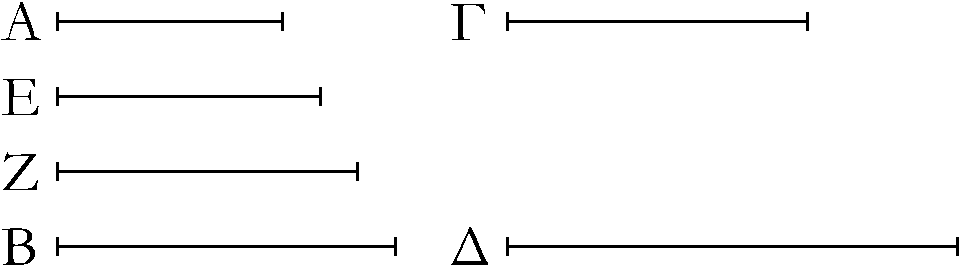
\includegraphics{Book08/fig25g.pdf}}

\gr{Δύο γὰρ ἀριθμοὶ οἱ Α, Β πρὸξ ἀλλήλουξ λόγον ἐθέτωσαν,
<ὸν κύβοξ ἀριθμὸξ ὁ Γ πρὸξ κύβον ἀριθμὸν τὸν Δ, κύβοξ
δὲ >έστω ὁ Α; λέγω [δή], <ότι καὶ ὁ Β κύβοξ ἐστίν.}

\gr{Ἐπεὶ γὰρ οἱ Γ, Δ κύβοι εἰσίν, οἱ Γ, Δ <όμοιοι
στερεοί εἰσιν; τῶν Γ, Δ >άρα δύο μέσοι ἀνάλογον ἐμπίπτουσιν
ἀριθμοί. <όσοι δὲ εἰξ τοὺξ Γ, Δ μεταχὺ κατὰ
τὸ συνεθὲξ ἀνάλογον ἐμπίπτουσιν, τοσοῦτοι καὶ εἰξ τοὺξ
τὸν α\kern -.7pt  ὐτὸν λόγον >έθονταξ α\kern -.7pt  ὐτοῖξ; <ώστε καὶ τῶν Α, Β δύο
μέσοι ἀνάλογον ἐμπίπτουσιν ἀριθμοί. ἐμπιπτέτωσαν οἱ Ε, Ζ.
ἐπεὶ ο>ῦν τέσσαρεξ ἀριθμοὶ οἱ Α, Ε, Ζ, Β ἑχῆξ ἀνάλογόν
εἰσιν, καί ἐστι κύβοξ ὁ Α, κύβοξ >άρα καὶ ὁ Β;
<όπερ >έδει δεῖχαι.}}

\ParallelRText{
\begin{center}
{\large Proposition 25}
\end{center}

If two numbers have to one another the
ratio which a cube number (has) to a(nother) cube number, and
the first is cube, then the second will also be cube.

% Removed epsf size command
\centerline{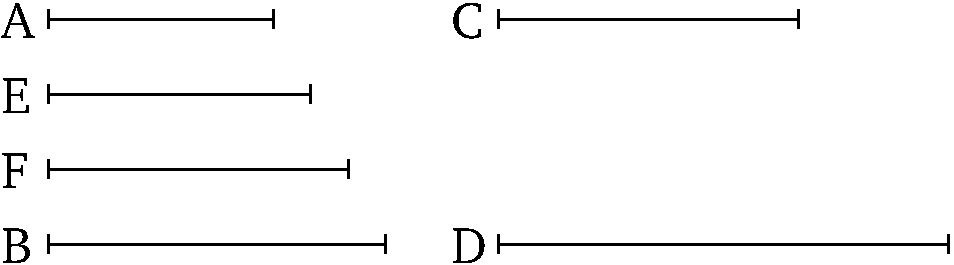
\includegraphics{Book08/fig25e.pdf}}

For  let two numbers, $A$ and $B$, have to one another the ratio which
the cube number $C$ (has) to the cube number $D$. And let $A$ be
 cube. [So] I say that $B$ is also  cube.
 
For since $C$ and $D$ are cube (numbers), $C$ and $D$ are (thus)
similar solid (numbers). Thus, two numbers fall
(between) $C$ and $D$  in mean proportion [Prop.~8.19]. And as many (numbers) as fall in between
$C$ and $D$  in continued proportion, so many also (fall)  in (between) those (numbers) having the same ratio as them (in continued proportion)
[Prop.~8.8].  And hence two numbers fall  (between) $A$ and $B$ in mean
proportion. Let $E$ and $F$ (so) fall.
Therefore, since the four numbers $A$, $E$, $F$, $B$ are continuously
proportional, and $A$ is  cube, $B$ (is) thus also 
cube [Prop.~8.23]. (Which is) the
very thing it was required to show.}
\end{Parallel}

%%%%%%
% Prop 8.26
%%%%%%
\pdfbookmark[1]{Proposition 8.26}{pdf8.26}
\begin{Parallel}{}{} 
\ParallelLText{
\begin{center}
{\large \ggn{26}.}
\end{center}\vspace*{-7pt}

\gr{Οἱ <όμοιοι ἐπίπεδοι ἀριθμοὶ πρὸξ ἀλλήλουξ λόγον
>έθουσιν, <ὸν τετράγωνοξ ἀριθμὸξ πρὸξ τετράγωνον
ἀριθμόν.}\\

% Removed epsf size command
\centerline{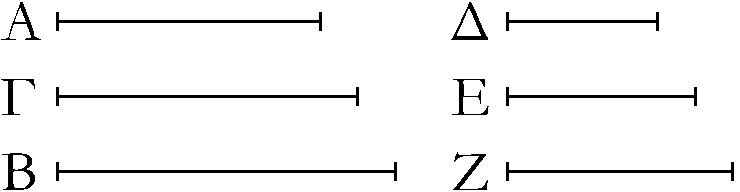
\includegraphics{Book08/fig26g.pdf}}

\gr{>'Εστωσαν <όμοιοι ἐπίπεδοι ἀριθμοὶ οἱ Α, Β; λέγω, <ότι ὁ Α
πρὸξ τὸν Β λόγον >έθει, <ὸν τετράγωνοξ ἀριθμὸξ πρὸξ τετράγωνον
ἀριθμόν.}

\gr{Ἐπεὶ γὰρ οἱ Α, Β <όμοιοι ἐπίπεδοί εἰσιν, τῶν Α, Β >άρα
ε~ἱξ μέσοξ ἀνάλογον ἐμπίπτει ἀριθμόξ. ἐμπιπτέτω
καὶ >έστω ὁ Γ, καὶ εἰλήφθωσαν ἐλάθιστοι ἀριθμοὶ τῶν
τὸν α\kern -.7pt  ὐτὸν λόγον ἐθόντων τοῖξ Α, Γ, Β οἱ Δ, Ε, Ζ; οἱ
>άρα >άκροι α\kern -.7pt  ὐτῶν οἱ Δ, Ζ τετράγωνοί εἰσιν. καὶ ἐπεί
ἐστιν ὡξ ὁ Δ πρὸξ τὸν Ζ, ο<ύτωξ
ὁ Α πρὸξ τὸν Β, καί εἰσιν οἱ Δ, Ζ τετράγωνοι, ὁ
Α >άρα πρὸξ τὸν Β λόγον >έθει, <ὸν τετράγωνοξ ἀριθμὸξ πρὸξ
τετράγωνον ἀριθμόν; <όπερ >έδει δεῖχαι.}}

\ParallelRText{
\begin{center}
{\large Proposition 26}
\end{center}

Similar plane numbers have to one another
the ratio which (some) square number (has) to a(nother) square number.

% Removed epsf size command
\centerline{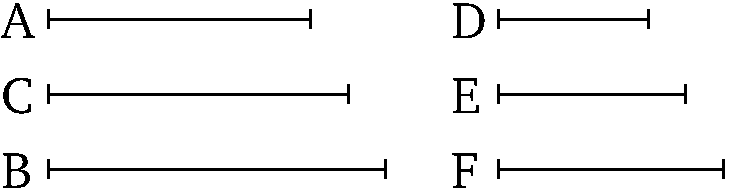
\includegraphics{Book08/fig26e.pdf}}

Let $A$ and $B$ be similar plane numbers. I say that $A$ has to $B$ the
ratio which (some) square number (has) to a(nother) square number.

For since $A$ and $B$ are similar plane numbers, one number thus
falls  (between) $A$ and $B$ in mean proportion [Prop.~8.18]. Let it (so) fall, and let it be $C$. 
And let the least numbers, $D$, $E$, $F$, having the same
ratio as $A$, $C$, $B$ be taken [Prop.~8.2].
The outermost of them, $D$ and $F$, are thus square 
[Prop.~8.2~corr.]. And since as $D$ is to $F$, so
$A$ (is) to $B$, and $D$ and $F$ are square, $A$ thus
has to $B$ the ratio which (some) square number (has) to a(nother)
square number. (Which is) the very thing it was required to show.}
\end{Parallel}

%%%%%%
% Prop 8.27
%%%%%%
\pdfbookmark[1]{Proposition 8.27}{pdf8.27}
\begin{Parallel}{}{} 
\ParallelLText{
\begin{center}
{\large \ggn{27}.}
\end{center}\vspace*{-7pt}

\gr{Οἱ <όμοιοι στερεοὶ ἀριθμοὶ πρὸξ ἀλλήλουξ λόγον >έθουσιν, <ὸν
κύβοξ ἀριθμὸξ πρὸξ κύβον ἀριθμόν.}

% Removed epsf size command
\centerline{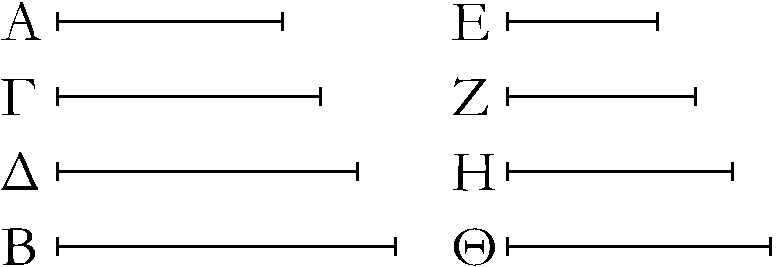
\includegraphics{Book08/fig27g.pdf}}

\gr{>'Εστωσαν <όμοιοι στερεοὶ ἀριθμοὶ οἱ Α, Β; λέγω, <ότι ὁ Α πρὸξ
τὸν Β λόγον >έθει, <ὸν κύβοξ ἀριθμὸξ πρὸξ κύβον ἀριθμόν.}

\gr{Ἐπεὶ γὰρ οἱ Α, Β <όμοιοι στερεοί εἰσιν, τῶν Α, Β >άρα δύο
μέσοι ἀνάλογον ἐμπίπτουσιν ἀριθμοί. ἐμπιπτέτ\-ωσαν οἱ Γ, Δ,
καὶ εἰλήφθωσαν ἐλάθιστοι ἀριθμοὶ τῶν τὸν α\kern -.7pt  ὐτὸν λόγον ἐθόντων
τοῖξ Α, Γ, Δ, Β >ίσοι α\kern -.7pt  ὐτοῖξ τὸ πλῆθοξ οἱ Ε, Ζ, Η, Θ; οἱ >άρα
>άκροι α\kern -.5pt  ὐτῶν οἱ Ε, Θ κύβοι εἰσίν. καί ἐστιν ὡξ ὁ Ε πρὸξ
τὸν Θ, ο<ύτωξ ὁ Α πρὸξ τὸν Β; καὶ ὁ Α >άρα πρὸξ τὸν Β λόγον
>έθει, <ὸν κύβοξ ἀριθμὸξ πρὸξ κύβον ἀριθμόν; <όπερ >έδει
δεῖχαι.}}

\ParallelRText{
\begin{center}
{\large Proposition 27}
\end{center}

Similar solid numbers have to one another the
ratio which (some) cube number (has) to a(nother) cube number.

% Removed epsf size command
\centerline{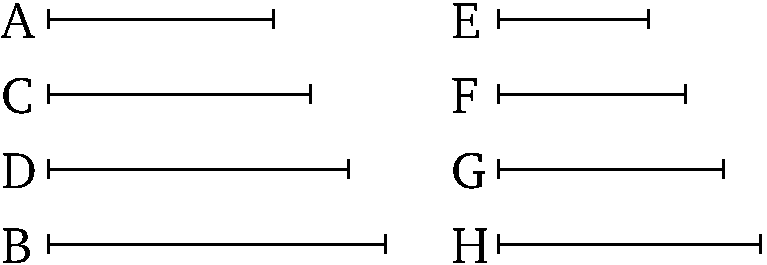
\includegraphics{Book08/fig27e.pdf}}

Let $A$ and $B$ be similar solid  numbers. I say that $A$ has to $B$
the ratio which (some) cube number (has) to a(nother) cube number.

For since $A$ and $B$ are similar solid (numbers), two numbers thus
fall
  (between) $A$ and $B$ in mean proportion [Prop.~8.19]. Let $C$ and $D$ have (so) fallen.
And let the least numbers, $E$, $F$, $G$, $H$, having the same
ratio as $A$, $C$, $D$, $B$, (and) equal in multitude to them, be taken [Prop.~8.2]. Thus, the outermost of them,
$E$ and $H$, are cube  [Prop.~8.2~corr.].
And as $E$ is to $H$, so $A$ (is) to $B$. And thus $A$ has to $B$ the ratio
which (some) cube number (has) to a(nother) cube number. (Which
is) the very thing it was required to show.}
\end{Parallel}
